%% Adaptado a partir de :
%%    abtex2-modelo-trabalho-academico.tex, v-1.9.2 laurocesar
%% para ser um modelo para os trabalhos no IFSP-SPO

\documentclass[
    % -- opções da classe memoir --
    12pt,               % tamanho da fonte
    openright,          % capítulos começam em pág ímpar (insere página vazia caso preciso)
    %twoside,            % para impressão em verso e anverso. Oposto a oneside
    oneside,
    a4paper,            % tamanho do papel. 
    % -- opções da classe abntex2 --schwinn
    % Opções que não devem ser utilizadas na versão final do documento
    %draft,              % para compilar mais rápido, remover na versão final
    paginasA3,  % indica que vai utilizar paginas em A3 
    MODELO,             % indica que é um documento modelo então precisa dos geradores de texto
    TODO,               % indica que deve apresentar lista de pendencias 
    % -- opções do pacote babel --
    english,            % idioma adicional para hifenização
    brazil              % o último idioma é o principal do documento
    ]{ifsp-spo-inf-ctds} % ajustar de acordo com o modelo desejado para o curso

% ---
% Pacotes importados para a utilização de referências
% ---

% ---
% Informações de dados para CAPA e FOLHA DE ROSTO
% ---
\titulo{DESENHO DA APLICAÇÃO - PROJETO TURMA DE ELITE}

% Trabalho individual
%\autor{AUTOR DO TRABALHO}

% Trabalho em Equipe
% ver também https://github.com/abntex/abntex2/wiki/FAQ#como-adicionar-mais-de-um-autor-ao-meu-projeto
\renewcommand{\imprimirautor}{
\begin{tabular}{lr}
     André Monteiro GOMES & SP3024059 \\
     Bianca Kaori HNG & SP3022455\\
     Luiz Henrique de Almeida e ALBUQUERQUE & SP3030199\\
     Natan da Fonseca LISBOA & SP3024784\\
     Patrícia Santos PASCHOAL & SP3022218
\end{tabular}
}


\disciplina{PI1A5 - Projeto Integrado I}

\preambulo{Trabalho apresentado ao Instituto Federal de Educação, Ciência e Tecnologia de São Paulo - Câmpus São Paulo - como parte dos requisitos para aprovação na disciplina Projeto Integrado I (PI1A5), do curso superior de Tecnologia em Análise e Desenvolvimento de Sistemas.}

\data{2021}

% Definir o que for necessário e comentar o que não for necessário
% Utilizar o Nome Completo, abntex tem orientador e coorientador
% então vão ser utilizados na definição de professor
\renewcommand{\orientadorname}{Professor:}
\orientador{DANIEL MARQUES GOMES DE MORAIS}


% ---


% informações do PDF
\makeatletter
\hypersetup{
        %pagebackref=true,
        pdftitle={\@title}, 
        pdfauthor={\@author},
        pdfsubject={\imprimirpreambulo},
        pdfcreator={LaTeX with abnTeX2 using IFSP model},
        pdfkeywords={abnt}{latex}{abntex}{abntex2}{IFSP}{\ifspprefixo}{trabalho acadêmico}, 
        colorlinks=true,            % false: boxed links; true: colored links
        linkcolor=blue,             % color of internal links
        citecolor=blue,             % color of links to bibliography
        filecolor=magenta,              % color of file links
        urlcolor=blue,
        bookmarksdepth=4
}
\makeatother
% --- 

% carregando aqui referencias quando utilizando BIBLATEX
\IfPackageLoaded{biblatex}{%
\addbibresource{referencias.bib}
\addbibresource{exemplos/abntex2-doc-abnt-6023.bib}
}{}

% ----
% Início do documento
% ----
\begin{document}


% Retira espaço extra obsoleto entre as frases.
\frenchspacing 

%somente para o exemplo, fica primeiro
%\newcommand{\urlmodelosimples}{https://www.overleaf.com/project/58a3a66af9bb74023ba1bd56}
\newcommand{\urlmodelo}{\url{\urlmodelosimples}}

\newcommand{\explicacao}[1]{\todo[nolist,inline,color=yellow]{#1}}
\newcommand{\explicacaoErro}[1]{\todo[nolist,inline,color=red]{ERRADO: #1}}

% Para facilitar mudanças no site a página 404 tem um redirecionamento pelas chaves
% utiliza diretamente esse sistema de redirecionamento
\newcommand{\dicasIvan}[1]{\href{https://dicas.ivanfm.com/404.html?key=#1}{https://dicas.ivanfm.com/#1}}

Esse documento foi feito a partir do modelo canônico do \abnTeX, o acesso ao \acs{pdf} pode ser feito em 
\urlmodelo. Esse modelo foi feito como exemplo para alunos do \ac{ifsp}.
\todo[inline]{Remover texto informativo inicial}

Este documento não pode ser considerado como um padrão a ser seguido em sua totalidade, ele tem como maior objetivo demonstrar como utilizar o \LaTeX\ para obter um documento atendendo ao máximo o padrão do \ac{ifsp} e \ac{abnt}.

Faça leitura dos arquivos fonte \LaTeX\ e não somente do \acs{pdf} gerado.
\todo{Fazer leitura das referências}

Algumas bibliotecas \LaTeX\ disponíveis no overleaf estão desatualizadas, para melhores resultados é recomendável a utilização de outro compilador utilizando as ultimas versões de todas bibliotecas

Leia com cuidado :
\begin{itemize}
    \item \dicasIvan{textos};
    
    \item exemplos de \LaTeX \space no \autoref{cap-exemplos};

    \item Cuidado para não cometer os erros indicados no \autoref{erros-comuns-capitulo} e \autoref{erros-projetos};
    
    \item Revisão de Textos no \autoref{revisao-de-textos};

    \item \autoref{elementos-nao-textuais} sobre elementos não textuais que fala sobre o maior problema dos alunos que é de tentar posicionar as ilustrações.
\end{itemize}

Um modelo para slides utilizando Beamer : \url{https://www.overleaf.com/read/qjrjhqwqbqqw}


Esse modelo ainda utiliza o abntex2cite
\todo[inline]{migrar do abntex2cite para biblatex-abnt \url{http://www.abntex.net.br/\#abntex3-e-biblatex-abnt}}


\noindent\hrulefill

\newpage


% -- lista de pendencias gerada pelo todonotes
% -- altere opções do usepackage para remover na versão final....
%\listoftodos
%\todo[inline]{remover lista de todo da versão final...}
%\newpage

% ----------------------------------------------------------
% ELEMENTOS PRÉ-TEXTUAIS
% ----------------------------------------------------------
\pretextual

% ---
% Capa
% ---
\imprimircapa

%--
% \newcounter{todocounter}
% \newcommand{\todonum}[2][]
% {\stepcounter{todocounter}\todo[#1]{\thetodocounter: #2}}

%\todonum[inline]{ajustar titulo do trabalho}
%\todonum[inline]{ajustar autor}
%\todonum[inline]{ajustar data}
%\todonum[inline]{ajustar preambulo}
%\todonum[inline]{ajustar curso}
%\todonum[inline]{ajustar disciplina}
%\todonum[inline]{ajustar departamento}
%\todonum[inline]{ajustar orientador/coorientador/professor(es)}
% ---

% ---
% Folha de rosto
% (o * indica que haverá a ficha bibliográfica)
% ---
\imprimirfolhaderosto
% \imprimirfolhaderosto*
% ---

% Quando registrado na biblioteca
%
% ---
% Inserir a ficha bibliografica
% ---

% Isto é um exemplo de Ficha Catalográfica, ou ``Dados internacionais de
% catalogação-na-publicação''. Você pode utilizar este modelo como referência. 
% Porém, provavelmente a biblioteca da sua universidade lhe fornecerá um PDF
% com a ficha catalográfica definitiva após a defesa do trabalho. Quando estiver
% com o documento, salve-o como PDF no diretório do seu projeto e substitua todo
% o conteúdo de implementação deste arquivo pelo comando abaixo:
%
% \begin{fichacatalografica}
%     \includepdf{fig_ficha_catalografica.pdf}
% \end{fichacatalografica}
\begin{fichacatalografica}
    \vspace*{\fill}                 % Posição vertical
    \hrule                          % Linha horizontal
    \begin{center}                  % Minipage Centralizado
    \begin{minipage}[c]{12.5cm}     % Largura
    
    \imprimirautor
    
    \hspace{0.5cm} \imprimirtitulo  / \imprimirautor. --
    \imprimirlocal, \imprimirdata-
    
    \hspace{0.5cm} \pageref{LastPage} p. : il. (algumas color.) ; 30 cm.\\
    
    \hspace{0.5cm} \imprimirorientadorRotulo~\imprimirorientador\\
    
    \hspace{0.5cm}
    \parbox[t]{\textwidth}{\imprimirtipotrabalho~--~\imprimirinstituicao,
    \imprimirdata.}\\
    
    \hspace{0.5cm}
        1. Palavra-chave1.
        2. Palavra-chave2.
        I. Orientador.
        II. Universidade xxx.
        III. Faculdade de xxx.
        IV. Título\\            
    
    \hspace{8.75cm} CDU 02:141:005.7\\
    
    \end{minipage}
    \end{center}
    \hrule
\end{fichacatalografica}
% ---



%Caso necessário
%% ---
% Inserir errata
% ---
\begin{errata}
Elemento opcional da \citeonline[4.2.1.2]{NBR14724:2011}. Exemplo:

\vspace{\onelineskip}


FERRIGNO, C. R. A. \textbf{Tratamento de neoplasias ósseas apendiculares com
reimplantação de enxerto ósseo autólogo autoclavado associado ao plasma
rico em plaquetas}: estudo crítico na cirurgia de preservação de membro em
cães. 2011. 128 f. Tese (Livre-Docência) - Faculdade de Medicina Veterinária e
Zootecnia, Universidade de São Paulo, São Paulo, 2011.

\begin{table}[htb]
\center
\footnotesize
\begin{tabular}{|p{1.4cm}|p{1cm}|p{3cm}|p{3cm}|}
  \hline
   \textbf{Folha} & \textbf{Linha}  & \textbf{Onde se lê}  & \textbf{Leia-se}  \\
    \hline
    1 & 10 & auto-conclavo & autoconclavo\\
   \hline
\end{tabular}
\end{table}

\end{errata}
% ---

%Obrigatório para trabalhos com bancas oficiais
%% ---
% Inserir folha de aprovação
% ---

% Isto é um exemplo de Folha de aprovação, elemento obrigatório da NBR
% 14724/2011 (seção 4.2.1.3). Você pode utilizar este modelo até a aprovação
% do trabalho. Após isso, substitua todo o conteúdo deste arquivo por uma
% imagem da página assinada pela banca com o comando abaixo:
%
% \includepdf{folhadeaprovacao_final.pdf}
%
\begin{folhadeaprovacao}

  \begin{center}
    {\ABNTEXchapterfont\large\imprimirautor}

    \vspace*{\fill}\vspace*{\fill}
    \begin{center}
      \ABNTEXchapterfont\bfseries\Large\imprimirtitulo
    \end{center}
    \vspace*{\fill}
    
    \hspace{.45\textwidth}
    \begin{minipage}{.5\textwidth}
        \imprimirpreambulo
    \end{minipage}%
    \vspace*{\fill}
   \end{center}
        
   Trabalho aprovado. \imprimirlocal, 24 de novembro de 2012:

   \assinatura{\textbf{\imprimirorientador} \\ Orientador} 
   \assinatura{\textbf{Professor} \\ Convidado 1}
   \assinatura{\textbf{Professor} \\ Convidado 2}
   %\assinatura{\textbf{Professor} \\ Convidado 3}
   %\assinatura{\textbf{Professor} \\ Convidado 4}
      
   \begin{center}
    \vspace*{0.5cm}
    {\large\imprimirlocal}
    \par
    {\large\imprimirdata}
    \vspace*{1cm}
  \end{center}
  
\end{folhadeaprovacao}
% ---


% ---- opcionais 
% % ---
% Dedicatória
% ---
\begin{dedicatoria}
   \vspace*{\fill}
   \centering
   \noindent
   \textit{ Este trabalho é dedicado a todos aqueles que lutam por um sistema educacional mais democrático e justo para todos.} 

%\todonum 
   
   \vspace*{\fill}
   

\end{dedicatoria}
% ---
% % ---
% Agradecimentos
% ---
\begin{agradecimentos}
Agradecemos ao nosso professor orientador Daniel Marques, que sempre que podia, nos guiou e tirou nossas dúvidas, nossos familiares e amigos, aos nossos colegas de turma e todos aqueles que apoiaram e acreditaram no nosso projeto.


\end{agradecimentos}
% ---
% % ---
% Epígrafe
% ---
\begin{epigrafe}
    \vspace*{\fill}
    \begin{flushright}
        \textit{``Ninguém ignora tudo. Ninguém sabe tudo. \\
        Todos nós sabemos alguma coisa. \\
        Todos nós ignoramos alguma coisa.\\
        Por isso aprendemos sempre. \\
        (Paulo Freire)}
    \end{flushright}
\end{epigrafe}
% ---

% -- resumo obrigatório
% % ---
% RESUMOS
% ---
% resumo em português
\setlength{\absparsep}{18pt} % ajusta o espaçamento dos parágrafos do resumo
\begin{resumo}

 \vspace{\onelineskip}

 A gamificação consiste no uso de mecânicas e características de jogos em atividades que, inicialmente, não aplicam os elementos dos jogos. O principal objetivo desse trabalho é apresentar a aplicação Turma de Elite, um sistema web de gestão de aprendizado que implementa conceitos de gamificação e possui como principal público-alvo os estudantes das redes de ensino, contemplando, em primeira instância, os alunos do 6$^\circ$ ao 9$^\circ$ ano do ensino fundamental, para depois abranger os outros níveis do ambiente escolar, inclusive visando o ensino superior. Serão abordados neste documento questões como a arquitetura e escopo do projeto, tecnologias utilizadas na aplicação e outros pontos relacionados ao sistema, bem como todo processo de produção do mesmo, considerando levantamentos e descartes efetuados. 
 Propõe-se, desse modo, criar uma alternativa tecnológica que promova um maior engajamento dos estudantes no processo de aprendizado, de modo que eles tenham uma maior motivação para adquirir conhecimento por meio dos estudos. Sob essa perspectiva, a gamificação pode ser considerada uma poderosa ferramenta de engajamento, sendo que o desenvolvimento de sistemas que apliquem tais conceitos é totalmente possível.
 
 Para o desenvolvimento da aplicação foi utilizado Angular para o front-end, Firebase authentication para a autenticação dos dados do usuário, servidor SMTP da Google para envio de e-mails de confirmação, o serviço S3 da Amazon para armazenar arquivos enviados pelos usuários, PostgreSQL como banco de dados, Spring Boot para criação e configuração da aplicação, Spring Data para auxiliar no acesso aos dados do banco de dados e Heroku para a hospedagem dos serviços.
 
 \vspace{\onelineskip}
 
 \textbf{Palavras-chave}: Gamificação. Sistema de gestão de aprendizado. Engajamento nos estudos.
 
\end{resumo}

% resumo em inglês
\begin{resumo}[Abstract]
 \begin{otherlanguage*}{english}
 
    \vspace{\onelineskip}
 
     Gamification consists in the use of mechanics and games features in activities that does not apply the game concepts initially. The main purpose of this paper is present the Turma de Elite application, a web Learning Management System that implements gamification concepts and have the education network students as the main target audience, contemplating, in the first instance, 6th to 9th elementary school students, to then cover the other education levels, including aiming the university education.
     This document will address subjects such as architecture, project scope, technologies used and other points related to the system, as well as the entire production process, considering surveys and disposals that were made.
     Thus, it is proposed to create a technological alternative that leads to greater engagement of the students in the learning process, so that they would be more motivated to acquire knowledge through their studies. From this perspective, it is proven that gamification is a powerful engagement tool, being that the development of systems that applies this concepts is totally possible.
     
    \todo[inline]{fazer tradução do resumo, não utilizar tradução automática}
   \vspace{\onelineskip}
   \noindent 
   \textbf{Keywords}: Gamification. Learning Management System. Engagement in studies.
 \end{otherlanguage*}
\end{resumo}


% ---
% inserir lista de ilustrações
% ---
\pdfbookmark[0]{\listfigurename}{lof}
\listoffigures*
\cleardoublepage
% ---

% ---
% inserir lista de tabelas
% ---
\pdfbookmark[0]{\listtablename}{lot}
\listoftables*
\cleardoublepage
% ---

% ---
% inserir lista de quadros
% ---
% \pdfbookmark[0]{\listofquadrosname}{loq}
% \listofquadros*
% \cleardoublepage
% ---

% % ---
% inserir lista de abreviaturas e siglas
% ATENCAO o SHARELATEX/OVERLEAF GERA O GLOSSARIO SOMENTE UMA VEZ
% CASO SEJA FEITA ALGUMA ALTERAÇÃO NA LISTA DE SIGLAS É NECESSARIO UTILIZAR A OPÇÃO :
% "Clear Cached Files" DISPONIVEL NA VISUALIZAÇÃO DOS LOGS 
% ---
% https://www.sharelatex.com/learn/Glossaries


% \ifdef{\printnoidxglossary}{
    % \printnoidxglossary[type=\acronymtype,title=Li% sta de abreviaturas e siglas,style=siglas]
    % \cleardoublepage
% }{}


% % ---
% inserir lista de símbolos
% ---
\begin{simbolos}
  \item[$ \Gamma $] Letra grega Gama
  \item[$ \Lambda $] Lambda
  \item[$ \zeta $] Letra grega minúscula zeta
  \item[$ \in $] Pertence
\end{simbolos}
% ---

% \todo[inline]{Remover lista de simbolos se não for necessário}


% ---
% inserir o sumario
% ---
\pdfbookmark[0]{\contentsname}{toc}
\tableofcontents*
% ---


% ----------------------------------------------------------
% ELEMENTOS TEXTUAIS
% ----------------------------------------------------------
\textual

% ----------------------------------------------------------
% Introdução
% ----------------------------------------------------------
\chapter[Introdução]{Introdução}
\section{Questão de pesquisa}
As atividades interativas proporcionadas pelos jogos eletrônicos poderiam fazer com que um aluno ganhasse interesse pelos estudos?

\section{Problematização}
A participação dos alunos nas aulas e atividades escolares é essencial para a evolução do aprendizado. Porém, é possível observar que apenas a rotina de horas de aula combinada a um grande volume de atividades com poucas recompensas imediatas tendem a fazer com que os estudos se tornem maçantes para a maioria dos alunos, resultando na falta de motivação para desempenhar suas obrigações escolares.

\section{Objetivos}
Este projeto visa desenvolver o sistema Turma de Elite, uma aplicação de gerenciamento de aprendizado que tem como objetivo integrar conceitos de \textit{gamificação} ao ensino, e deste modo se tornar uma ferramenta que busca auxiliar todo corpo docente e discente de uma instituição escolar.

Para o corpo docente, a ferramenta contará com funcionalidades que permitam acompanhar o desenvolvimento do aluno e modelar desafios, atividades e recompensas.

Para o corpo discente, a aplicação implementará funcionalidades que buscam promover o engajamento dos alunos nas aulas, acrescentando ao processo de realizar exercícios e avaliações, uma dinâmica semelhante aos jogos atuais onde ao completar um desafio, ganham-se recompensas, aumenta-se de nível e desbloqueia novos desafios.

\subsection{Objetivo Principal}
De modo geral, o projeto Turma de Elite tem a missão de promover um maior interesse dos alunos nos estudos por meio do aumento de fatores motivacionais na realização de tarefas, utilizando a tecnologia como elemento auxiliador nesse processo.

\subsection{Objetivos Secundários}
Tendo em vista a inserção tecnológica ocorrendo cada vez mais cedo na sociedade, coloca-se como objetivo secundário (e futuro) a maior disseminação da tecnologia no ambiente estudantil, de maneira benéfica.

\section{Justificativa}
Hoje em dia, já é possível encontrar plataformas educacionais online que aplicam o conceito de \textit{gamificação} para promover a aprendizagem do aluno. Entretanto, ao analisar as soluções existentes no mercado, percebe-se que a maioria possui uma deficiência em comum, não possuir código aberto. Este tipo de aplicação possui conteúdo engessado e é fortemente atrelado ao fabricante (\textit{vendor lock-in}). 

No contexto educacional brasileiro, sabe-se que embora as escolas sejam obrigadas a seguir uma grade fixa de disciplinas e conteúdos de base, cada instituição possui sua maneira única de ofertá-lo aos seus alunos. Deste modo, surgiu o interesse de desenvolver uma solução que aplique conceitos de \textit{gamificação} na educação para motivar os alunos, mas que ao mesmo tempo seja flexível às necessidades dos diferentes clientes. 

Ademais, partindo de uma base de dados que será alimentada ao longo da utilização da aplicação, será possível desenvolver visões gerenciais que permitam aos diretores, pedagogos e professores acompanharem a evolução dos seus alunos, bem como diagnosticarem possíveis problemas e tomarem decisões para superá-los.

\section{Análise de concorrência}
\subsection{\textit{Khan Academy}}
Tomando uma plataforma como a Khan Academy, que utiliza conceitos de \textit{gamificação} para a execução de atividades, nota-se que ela não utiliza o conceito de \textit{tiers} para ranquear os alunos, por exemplo. Esse conceito compreende ao agrupamento de estudantes em ligas diferentes de acordo com o desempenho.

Outro diferencial em relação ao Khan Academy, são as funcionalidades de customização de atividades, parametrização de turmas e conquistas que permitem que a Turma de Elite se adapte não só a diferentes escolas como também às categorias de ensino remoto e à distância.

\subsection{\textit{Academy LMS}}
Essa outra solução, por sua vez, já possui suporte para múltiplas visões de usuário.
Entretanto, como ela não possui código aberto, uma forma de obtenção de lucro encontrada foi a cobrança por meio de uma assinatura.

\subsection{\textit{Axonify}}
Esse sistema de gestão de aprendizagem possui algumas funcionalidades interessantes no que diz respeito à implementação de \textit{gamificação}, como pontos, conquistas, medalhas e \textit{rankings}. Entretanto, tal solução também não possui código ou visão para um administrador. 

\subsection{\textit{Matrix LMS}}
Dentre as soluções verificadas, essa se mostrou a solução mais completa, uma vez que possui todas as visões de usuário que a Turma de Elite pretende implementar (aluno, professor e gestor). Entretanto, uma grande desvantagem dela é o custo, uma vez que, além de uma assinatura ser cobrada para continuar utilizando a plataforma, os materiais oferecidos também são pagos.  

\subsection{\textit{Talent LMS}}
Ao analisar o \textit{Talent LMS}, pode-se constatar algumas ausências importantes para um sistema de aprendizagem gamificado, como a premiação com medalhas. Apesar disso, esse sistema compensa tal ausência com a implementação de pontos e níveis.

\subsection{\textit{Moodle} + \textit{Level Up}!}
Uma outra opção possível para gamificar o ensino é a incorporação de um \textit{plugin} que ofereça ferramentas de gamificação a um sistema de \textit{LMS} já consolidado no mercado. Ao analisar as funcionalidades de um \textit{plugin} de \textit{gamificação} \textit{open source} chamado \textit{"Level Up!"}, nota-se que ele não contempla algumas funcionalidades para sua utilização no contexto de gestão de uma instituição de ensino, como a visão de gestor, por exemplo.

A comparação sintetizada de todos os sistemas analisados pode ser vista na tabela abaixo:

\ABNTEXfontereduzida
\begin{table}[htb]
\centering
\caption{Análise comparativa entre as plataformas de gestão de aprendizado}
\label{tabela-correta-equipamento}
\begin{tabular}{|m{2.3cm}|m{1.8cm}|m{1.8cm}|m{1.5cm}|m{1.5cm}|m{1.2cm}|m{1.5cm}|m{1.3cm}|m{1.8cm}}
\hline
{\thead{}} & \thead{Khan\\ Academy} & \thead{Academy\\ LMS} & \thead{Axonify} & \thead{Matrix \\LMS} & 
\thead{Talent \\ LMS} & 
\thead{Moodle \\+ Level\\ Up!} &
\thead{Turma\\ de \\elite} \\ \hline
    Código aberto               &   &   &   &   & X & X & X               \\ \hline
    Customização de atividades  &   & X & X & X & X & X & X               \\\hline
    Medalhas                    & X & X &   & X &   & X & X               \\ \hline
    Tiers / ligas               &   &   &   &   &   &   & X               \\ \hline
    Leaderboards                & X & X & X & X & X & X & X               \\ \hline
    Visão do Gestor             &   &   &   & X &   &   & X \\ \hline   
\end{tabular}
\fonte{Os autores}
\end{table}

% Para facilitar a manutenção é sempre melhore criar um arquivo por capitulo, para exemplo isso não é necessário 
% % Para facilitar a manutenção é sempre melhore criar um arquivo por capitulo, para exemplo isso não é necessário 

%---------------------------------------------------------------------------------------
\chapter{Modelo Teórico e Pressupostos (ou Hipóteses) da Pesquisa}
\explicacao{Para trabalho da Pós Graduação}
\lipsum[5-10]




%---------------------------------------------------------------------------------------
\chapter{Métodos de Pesquisa}
\explicacao{Para trabalho da Pós Graduação}
\lipsum[3]

\section{Tipo de Pesquisa}
\lipsum[3-5]

\section{Plano Amostral (se Pesquisa Quantitativa)}
\lipsum[3-5]

\section{Instrumento de Pesquisa e Escalas Utilizadas (Escalas se Pesquisa Quantitativa)}
\lipsum[3-5]

\section{Coleta de Dados}
\lipsum[3-5]

\section{Análise de Dados}
\lipsum[3-5]


%---------------------------------------------------------------------------------------
\chapter{Resultados da Pesquisa}
\explicacao{Para trabalho da Pós Graduação}
\lipsum[2]

\section{Assunto 1}
\lipsum[3-5]

\section{Assunto 2}
\lipsum[3-5]

\section{Assunto 3}
\lipsum[3-5]

\section{Discussão dos Resultados Observados}
\lipsum[3-5]

%---------------------------------------------------------------------------------------






% ---
% Capitulo de revisão de literatura
% ---
\chapter{Revisão da Literatura}

\section{\textit{Learning Management System}}
Os \textit{LMS} – plataformas de apoio à aprendizagem - surgiram para dar apoio à formação a distância online. As plataformas facilitam a disponibilização de recursos em diferentes formatos como texto, vídeo e áudio, apontadores para sites, avisos, interação professor-alunos através de ferramentas de comunicação, ferramentas de apoio à aprendizagem colaborativa e registro das atividades realizadas pelos alunos \cite{rentabilizacao-ens-basico-e-secundario:2007}.

\section{\textit{Gamificação}}
A \textit{gamificação} é uma técnica que envolve dinâmicas, mecanismos e elementos dos \textit{videogames} e os aplica em contextos da vida real. O principal objetivo é engajar as pessoas para que mudem alguns comportamentos, com o propósito de alcançar resultados relacionados a objetivos específicos.


A \textit{gamificação} surge justamente para auxiliar nessa demanda. Em situações em que o engajamento é precário, é possível estabelecer um estímulo extra em contextos que nada têm a ver com jogos, como ambientes corporativos e educacionais. \cite{gamificacao-corporativa:2017}

\section{Recompensa}
A recompensa se refere a um prêmio ou retribuição por algo \cite{dicio-recompensa:2009}


Todos gostam de se sentir valorizados por aquilo que produzem. Assim é importante que os gestores se lembrem de implementar alguns mecanismos de recompensas que motivem os colaboradores. \cite{gamificacao-corporativa:2017}


Em uma pesquisa realizada por uma empresa americana chamada \textit{Aberdeen Research}, constatou-se que mais da metade dos entrevistados associam a motivação com o reconhecimento por performance, conforme mostra o gráfico abaixo:

\begin{figure}[htb]
    \centering
	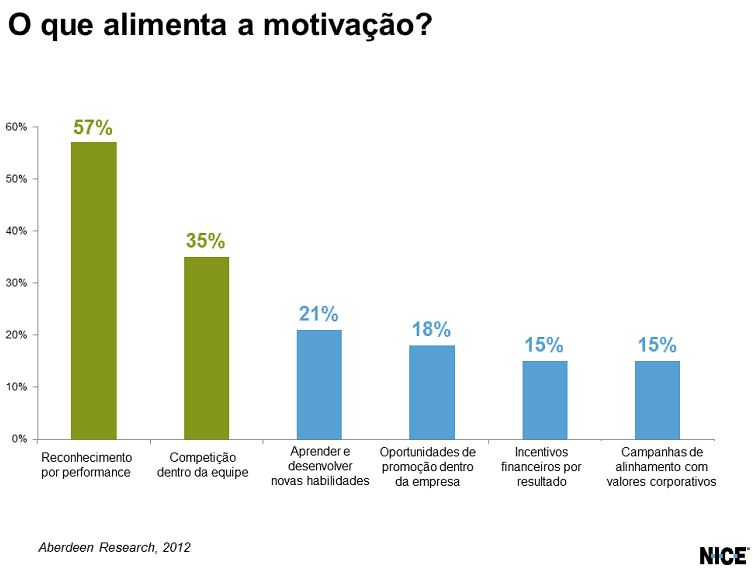
\includegraphics[width=16cm]{recompensa.jpg}
	\caption{\label{recompensa} O que alimenta a motivação?}
	\fonte{\cite{grafico-motivacao:2012}}
\end{figure}
\FloatBarrier


\section{Tecnologias}
\subsection{Java}
Java é uma linguagem de programação e plataforma computacional lançada pela primeira vez pela Sun Microsystems em 1995.
Para criar \textit{applets} e aplicações Java, são necessárias ferramentas de desenvolvimento como o JDK. O JDK inclui o Java Runtime Environment, o compilador Java e as APIs Java. É fácil começar a desenvolver programas em Java, tanto para os novos programadores quanto para os experientes \cite{java:2016}.
No projeto Turma de Elite, a linguagem de programação Java será utilizada no \textit{back-end}, apoiado pelo \textit{framework} Spring e seus componentes.

\subsection{Spring}
O Spring Framework fornece um modelo abrangente de programação e configuração para aplicativos empresariais modernos baseados em Java - em qualquer tipo de plataforma de implantação.

Um elemento-chave do Spring é o suporte de infraestrutura no nível do aplicativo: o Spring se concentra na "canalização" dos aplicativos corporativos para que as equipes possam se concentrar na lógica de negócios no nível do aplicativo, sem vínculos desnecessários com ambientes de implementação específicos \cite{spring:2021}.

\subsection {Angular}
Angular é uma plataforma de desenvolvimento, construída em 
TypeScript, que inclui:
\begin{itemize}
\item Uma estrutura baseada em componentes para a construção de aplicativos da \textit{web} escaláveis;
\item Uma coleção de bibliotecas bem integradas que cobrem uma ampla variedade de recursos, incluindo roteamento, gerenciamento de formulários, e comunicação cliente-servidor;
\item Um conjunto de ferramentas de desenvolvedor capaz de ajudar a desenvolver, construir, testar e atualizar o código \cite{angular:2021}.
\end{itemize}

Será utilizado o Angular como \textit{framework} para o \textit{front-end} do nosso projeto.

\subsection{MySQL}
Para armazenamento de dados foi escolhido o MySQL. Esse é o banco de dados de código aberto mais popular do mundo. Com seu desempenho comprovado, confiabilidade e facilidade de uso, o MySQL se tornou a principal escolha de banco de dados para aplicativos baseados na web, usados por propriedades da \textit{web} de alto perfil, incluindo Facebook, Twitter, YouTube, Yahoo! dentre outros \cite{mysql:2021}.

\subsection{GitHub}
O GitHub oferece um serviço de hospedagem de repositório Git baseado em nuvem, tornando assim muito mais fácil para que indivíduos e equipes usem o Git para controle de versão e colaboração.

A interface do GitHub é amigável o suficiente para que até programadores novatos possam utilizar o Git com facilidade. Sem o GitHub, seria necessário um pouco mais de conhecimento técnico e o uso da linha de comando para o uso do Git \cite{github:2021}.

\subsection{SVN}
Subversion (SVN) é um sistema de controle de versão de código aberto. Fundado em 2000 pela CollabNet, Inc., o projeto e o \textit{software} Subversion tiveram um sucesso incrível na última década. O Subversion tem desfrutado e continua a ter ampla adoção tanto na arena do código aberto quanto no mundo corporativo \cite{svn:2021}.

Durante o desenvolvimento, serão utilizados o GitHub e o SVN para o versionamento de código.

\subsection{Heroku}
Heroku é uma plataforma em nuvem que permite às empresas criar, entregar, monitorar e dimensionar aplicativos, sendo a maneira mais rápida de ir da ideia à URL.

A plataforma foca incansavelmente em aplicativos e na experiência do desenvolvedor em torno de aplicativos. O Heroku permite que empresas de todos os tamanhos adotem o valor dos aplicativos \cite{heroku:2021}.

\subsection{Travis CI}
Travis CI é um serviço de integração onde é possível sincrinizar projetosde código aberto hospedados no GitHub \cite{travis:2021}.

\subsection{Firebase Hosting}
O Firebase Hosting é um recurso de hospedagem de conteúdo da \textit{web} de nível de produção para desenvolvedores, sendo possível facilmente implantar apps da \textit{web} de forma rápida e exibir conteúdo estático e dinâmico a uma rede de distribuição de conteúdo (CDN) global \cite{hosting:2020}.

O \textit{back-end} da aplicação será hospedado no Heroku, utilizando como plataformade CI, o Travis. O \textit{front-end} da aplicação será hospedado com o serviço Firebase Hosting, do Google.

\subsection{Firebase Authentication}
A maioria dos \textit{apps} precisa reconhecer a identidade do usuário. Ter essa informação permite que um \textit{app} salve os dados do usuário na nuvem com segurança e forneça a mesma experiência personalizada em todos os dispositivos do usuário \cite{authentication:2020}.

O Firebase Authentication fornece serviços de \textit{back-end}, SDKs fáceis de usar e bibliotecas de IU prontas para autenticar usuários no seu aplicativo. Ele oferece suporte à autenticação usando senhas, números de telefone, provedores de identidade federados conhecidos, como Google, Facebook e Twitter, entre outros.

Para dar suporte à autenticação de usuário no sistema, será utilizado o Firebase Authentication.

\chapter{Gerenciamento do Projeto}
O gerenciamento do projeto funcionará conforme descrito nos tópicos a seguir: 

\section{Metodologia de Gestão}
A metodologia de gerenciamento de projeto adotada é baseada no Scrum.

O Scrum é um \textit{framework} para gestão de projetos que tem como objetivo agilizar o processo de desenvolvimento do \textit{software} e responder rapidamente às mudanças. Ela é composta por cerimônias e tem como um dos pilares as \textit{sprints}, ou seja, um conjunto de atividades para um determinado tempo. 

As atividades de uma \textit{sprint} serão planejadas em uma \textit{Sprint Planning}, que é a primeira cerimônia e tem como principal objetivo a definição das entregas para o final da \textit{sprint}. Nessa cerimônia será criado o Sprint Backlog em um arquivo em Excel, que contém as atividades e suas principais informações, como o responsável, o status, podendo ser \textit{To Do} (a fazer), \textit{Doing} (fazendo) e \textit{Done} (feito), e a data de conclusão. 

Após o planejamento da \textit{sprint}, a execução das atividades será iniciada. Então, reuniões de acompanhamento serão necessárias para ver o andamento do projeto e a identificação e possível resolução de impedimentos. Por isso, \textit{checkpoints} semanais acontecerão nas terças-feiras às 19h30 ao longo da sprint.

No último dia da \textit{sprint}, às 19h30, será feito uma reunião para revisão das entregas, a chamada Sprint Review, na qual será identificado o que foi entregue com sucesso, o que não foi concluído e também possíveis mudanças no Product Backlog. 

Após a \textit{Sprint Review}, será feito uma reunião de retrospectiva, a \textit{Sprint Retrospective}, para avaliar o desempenho da equipe, o andamento do projeto e possíveis melhorias para a próxima \textit{sprint}. A Sprint Planning da \textit{sprint} seguinte será realizado logo após a Sprint Review da anterior.

Todas as reuniões acontecerão através do \textit{Google Meet}.
Para eventuais dúvidas, alinhamentos e possíveis urgências será utilizado o \textit{WhatsApp Messenger} e, se necessário, reuniões no \textit{Google Meet}. 


\section{Organização da Equipe}
As atividades foram divididas entre os integrantes da equipe segundo as habilidades e interesses de cada um, levando-se em consideração também o nível de dificuldade de cada frente.

Desse modo, o André focará na frente de desenvolvimento do sistema, portanto a parte de preparação do ambiente, desenvolvimento \textit{back-end} e \textit{front-end} serão suas principais atividades, mas também atuará na frente de documentação na parte de elaboração, quando na fase inicial do projeto, e como suporte, ao longo dele.

A Bianca será a gerente de projetos, sendo a responsável por organizar a equipe e por garantir as entregas do projeto. Será responsável também pela postagem no blog semanalmente e auxiliará na elaboração da documentação e na criação dos vídeos. E poderá auxiliar nas outras frentes conforme houver necessidade.

O Luiz atuará principalmente na frente da documentação e auxiliará no desenvolvimento \textit{back-end}, sobretudo na parte de testes, e \textit{front-end}, na estilização das telas. Ele auxiliará também na frente dos vídeos e poderá desempenhar outras funções conforme houver necessidade.

O Natan focará na documentação, mas também auxiliará no desenvolvimento do \textit{back-end}, na parte de testes e no desenvolvimento da aplicação em si. Será o principal responsável pela criação, edição e postagem dos vídeos e também poderá atuar nas outras frentes conforme houver necessidade.

A Patricia terá como principal foco a documentação, principalmente a elicitação de requisitos e definição do escopo. Ela cuidará também da frente dos Dados da aplicação e auxiliará no \textit{front-end}, sobretudo na parte de protótipos de telas. E poderá auxiliar nas outras frentes conforme houver necessidade.


\section{Gestão de Tempo}

Baseando-se no Scrum, a gestão do tempo será feita pelas \textit{sprints}. Cada \textit{sprint} terá a duração de duas semanas e, no total, serão seis \textit{sprints}, com previsão de datas de início e de fim conforme descrito na Tabela 2. 

\ABNTEXfontereduzida
\begin{table}[htb]
\centering
\caption{Data de início e data fim de cada \textit{sprint}}
\label{tab-exemplo}
\begin{tabular}{|c|c|c|}
   \hline
   \thead{Sprint} & \thead{Data Início}  & \thead{Data Fim}   \\\hline
    1 & 10/05/21 & 25/05/21 \\\hline
    2 & 25/05/21 & 08/06/21 \\\hline
    3 & 08/06/21 & 22/06/21 \\\hline
    4 & 22/06/21 & 06/07/21 \\\hline
    5 & 06/07/21 & 20/07/21 \\\hline
    6 & 20/07/21 & 09/08/21 \\\hline
\end{tabular}
\fonte{Os autores}
\end{table}

As atividades priorizadas para cada \textit{sprint} serão baseadas no cronograma da disciplina e serão agrupadas visando a sua finalização até o final da \textit{sprint}, mas dependendo da dificuldade da atividade, ela poderá ser iniciada em uma \textit{sprint} e terminar em outra.

\chapter{Arquitetura de solução}
\section{Arquitetura da solução apresentada}
A arquitetura da solução proposta será baseada, de uma forma geral, na arquitetura MVC. Este modelo é apresentado em camadas que separam a apresentação e a interação de dados no sistema. É estruturado em três componentes: O modelo é responsável pelo gerenciamento dos dados, a visão que gerencia a apresentação dos dados e o controlador, responsável por intermediar a comunicação entre os eventos gerados pelo usuário na interface e o modelo \cite{engenharia-de-software:2018}

O diagrama apresentado pela Figura 2, mostra o modelo arquitetural adotado.

\begin{figure}[htb]
    \centering
	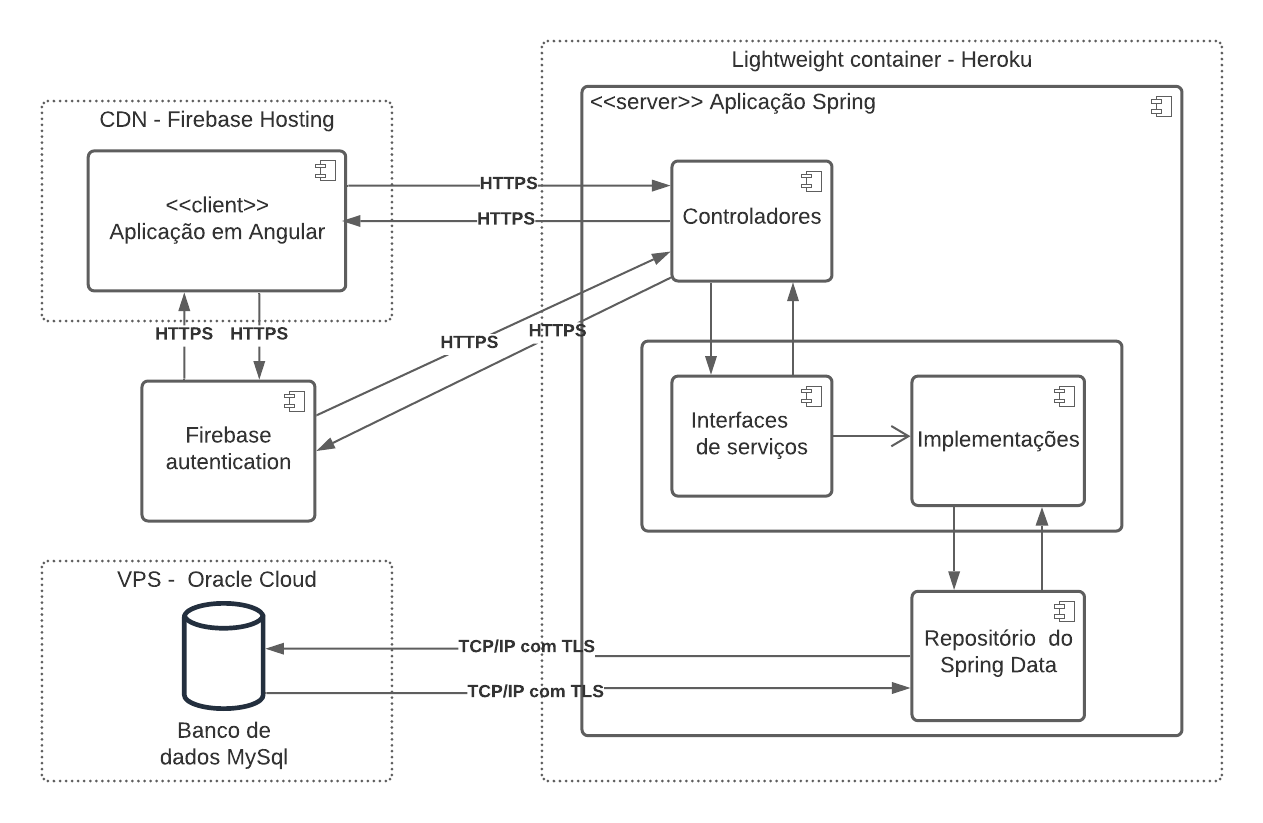
\includegraphics[width=16cm]{figura2.jpeg}
	\caption{\label{fig_logo} Arquitetura da solução.}
	\fonte{Os autores}
\end{figure}
 
De modo a desenvolver uma aplicação que busca garantir uma boa usabilidade, e capaz de aproveitar os recursos disponíveis da melhor forma, para a interface do usuário (\textit{front-end}) será adotado o modelo arquitetural Single Page Aplication (SPA). 

Neste modelo, a maioria dos recursos necessários é carregada na inicialização da aplicação, fazendo com que não seja necessário recarregar a página durante o uso. A única mudança que ocorre é a dos dados, que são trafegados entre o servidor e o cliente.

Conforme o diagrama apresentado pela Figura 2, as camadas que compões a solução utilizam as seguintes infraestruturas para hospedagem:
\begin{itemize}
\item CDN (Firebase Hosting): infraestrutura responsável por hospedar a aplicação em Angular, da camada de visão. Um serviço de hospedagem, que tem como base o armazenamento em SSD e uma CDN, totalmente gerenciado para conteúdo estático e dinâmico.
\item  Lightweight container (Heroku): infraestrutura responsável por hospedar a aplicação Spring, da camada controladora. A tecnologia utilizada pelo Heroku, utiliza o conceito de \textit{containers} que empacota o código e as dependências do aplicativo abstraindo o gerenciamento do \textit{hardware}, levando a simplificação do desenvolvimento e o aumento da produtividade.
\item VPS (Oracle Cloud): infraestrutura responsável por hospeda o banco de dados da aplicação. Esta infraestrutura oferece um alto poder de computação e segurança.
\end{itemize}

\section{Arquitetura de comunicação entre as camadas}
A comunicação entre a camada de visão e a camada controladora, será realizada via protocolo HTTPS. Este protocolo acrescenta uma camada a mais de segurança à aplicação, uma vez que utiliza a criptografia na transferência de recursos.

Já a comunicação entre os controladores e banco de dados, será realizada via TCP/IP acrescido do protocolo TLS que aumenta a segurança através de criptografia, a interoperabilidade, a extensabilidade e a eficiência;

\section{Necessidade de escalabilidade}
Como a aplicação inicialmente será destinada para utilização de um pequeno grupo de usuários, não haverá necessidade de escalabilidade.

\chapter {Segurança}
\section {Critérios de Segurança, Privacidade e Legislação}
Todos os dados e informações pessoais inseridas para cadastramento serão mantidos em sigilo pelo sistema, como previsto na Lei Geral de Proteção de Dados (LGPD), que regulamenta e controla processos relacionados a dados pessoais, visando proteger a liberdade e privacidade dos usuários.

Para realizar tal proteção de dados, seguiremos alguns pontos vitais para que os dados estejam guardados da maneira mais segura possível, seguindo os \textbf{Pilares da Segurança da Informação}.
\section {Pilares}
\begin{itemize}
\item \textbf{Confidencialidade}: garante que as informações estarão acessíveis somente para pessoas autorizadas, exigindo autenticação para restringir acessos;
\item \textbf{Integridade}: mantém a origem das informações conforme foram armazenadas, sem alterá-las;
\item \textbf{Disponibilidade}: faz com que os dados estejam disponíveis para usuários autorizados a qualquer momento que for necessário;
\item \textbf{Autenticidade}: identifica e registra usuários que estejam enviando ou modificando informações, para que essa ação seja documentada;
\end{itemize}


\chapter{Manutenibilidade da aplicação}

\section{Testes automatizados e análise estática}

Como o \textit{back-end} da aplicação será desenvolvido em Java, a ferramenta adotada para automatização de testes é o JUnit. O JUnit é um \textit{framework} de código aberto que auxilia o desenvolvimento de testes que verificam o funcionamento das classes e seus métodos. Ademais, a utilização do JUnit permite que toda estrutura de testes criada, seja executada a cada atualização da aplicação  de modo a garantir sua estabilidade e integridade.

No \textit{front-end} serão adotados os \textit{frameworks} de testes para Angular; Jasmine e Karma. Com o Jasmine, os testes poderão ser escritos de maneira independente do navegador e de bibliotecas para seu funcionamento. O Karma será utilizado para automatizar testes e executá-los para diversos navegadores a partir de um único comando. Com o Karma, além de testes unitários, também é possível realizar testes de integração e e2e.

Todas as ferramentas escolhidas serão configuradas com servidores de integração contínua (CI) de modo a manter o projeto livre de erros e inconsistências.

A análise estática do código no \textit{back-end} será realizada pela ferramenta \textit{Deep Source}. A ferramenta possui integração nativa com o GitHub que permite revisão do código durante todo processo de desenvolvimento do projeto, além de permitir rastrear métricas de código como cobertura de testes e de documentação. No \textit{front-end} a análise será realizada pelo próprio Eslint Schematics do Angular.

\section{Sistemas de \textit{log}}
Gerenciar os \textit{logs} da aplicação é essencial para manter sua integridade. Com os \textit{logs} é possível analisar as operações internas da aplicação, permitindo uma maior rastreabilidade que fornecem informações necessárias para resolução de possíveis problemas na aplicação.

O sistema de \textit{log} Journalctl foi adotado para o MySql. Ele será responsável por registrar os logs de entrada e saída da \textit{console}. 
Para o \textit{back-end} será utilizado o Simple Logging Facade for Java (SLF4J) com saída para o Heroku.  Nos logs do Heroku será possível visualizar: 
\begin{itemize}
\item Logs do aplicativo através do comando “--source app”;
\item Registros do sistema através do comando “--source heroku”;
\item Logs de \textit{API} através do comando “--source app --dyno api”.
\end{itemize}

No \textit{front-end} será utilizado o Cloud Logging do Firebase Hosting com o padrão de objeto console recomendado para desenvolvimento Web. Com essa ferramenta é possível visualizar:
\begin{itemize}
\item Logs com nível de registro INFO com os comandos "console.log()" e console.info();
\item Logs com nível de registro ERROS com os comandos "console.warn()" e "console.error()";
\item Mensagens internas com nível de registro DEBUG.
\end{itemize}
\section{Integração contínua}
O processo de integração contínua se inicia a partir da liberação de uma nova funcionalidade; através do \textit{pull request}, os desenvolvedores serão notificados da necessidade de realizar o \textit{merge}; neste momento, a equipe deverá se reunir para realizar a revisão do código. Esta revisão inclui a análise dos resultados dos testes configurados, caso todas as métricas de código seja atingida, é realizado um \textit{merge} com a branch develop. 

Quando houver a necessidade de realizar o \textit{deploy} da aplicação, basta apenas realizar o \textit{merge} com a branch release. Nela, a \textit{build} da aplicação será feita de forma automática, e a aplicação estará atualizada no servidor. 

A ferramenta escolhida para automatizar o processo de \textit{build} de aplicação e  apoiar a equipe no processo de CI e CD é o Travis CI.

\section{\textit{Coding Convention}}
Para a solução será adotada serão adotadas as diretrizes padrões da própria linguagem de programação. Para nomenclatura tanto o Java quanto o Typescript utilizam o UpperCamelCase para classes e lowerCamelCase para variáveis e métodos. A nomenclatura das também deverá ser mnemônica, isto é, deverá indicar à intenção de seu uso.

\section{\textit{Design Pattern}}
A aplicação contará com o padrão de projeto Observer. Este padrão de projeto do tipo comportamental define um mecanismo de assinatura que notifica os objetos observadores a respeito dos eventos que acontecem a um objeto observado. 

Este padrão é amplamente utilizado pelo no Angular, \textit{framework} adotado no desenvolvimento da do \textit{front-end} da aplicação. Nele, os observáveis apoiam a transmissão de mensagens entre os componentes da aplicação, sejam elas mensagens literais, mensagens ou eventos.

\chapter{Escopo do Projeto}
A proposta de projeto é uma aplicação \textit{web} voltada para auxiliar no acompanhamento da evolução no rendimento dos alunos nas atividades escolares.

\section{Mínimo Produto Viável (MVP)}
Considerando a rotina básica das escolas de ensino fundamental no Brasil, para o MVP, a aplicação contará com o módulo de cadastros que permitirá que o usuário (coordenador, diretor ou pedagogo) realize o cadastro de turmas, disciplinas, gestores e alunos.

Além da configuração básica, o gestor poderá atribuir os professores e alunos às turmas e disciplinas previamente cadastradas. Ademais, deverá configurar a estrutura de conquistas e os parâmetros para que sejam alcançados pelos alunos.

Ao acessar a aplicação, o professor poderá visualizar as turmas e disciplinas atribuídas a ele. Para cada turma/disciplina ele poderá visualizar o ranking dos alunos, inserir e receber as atividades deles.

Quando o aluno acessar a aplicação, o mesmo poderá visualizar as atividades pendentes e o painel de conquistas que apresentará as conquistas alcançadas e não alcançadas por ele. Ademais, poderá visualizar o ranking da turma, sua posição em relação aos seus amigos e a pontuação necessária para que ele suba para a liga (\textit{tiers}) imediatamente mais alta.

A aplicação também fornecerá um \textit{dashboard} que conterá gráficos com visões gerenciais que indicam o desempenho por turma e por aluno. Esse \textit{dashboard} estará disponível apenas para  usuários com o perfil gestor.
As funcionalidades a serem implementadas estão descritas com mais detalhes nos subcapítulos a seguir. 

\subsection{Login e perfis}
O módulo de acesso permitirá que usuários cadastrados acessem o sistema; todos os processos relacionados à definição e reinicialização de senha estão contemplados neste módulo. Também será possível definir, para um determinado perfil, quais são as suas permissões de acesso.
Inicialmente, contempla-se nesta proposta quatro categorias de perfil de acesso: 

\begin{itemize}
\item \textbf{Perfil aluno}: poderá acessar as disciplinas referentes à turma que ele foi inserido, painel de atividades, painel de conquistas, sua posição no ranking e os alunos que ocupam os três primeiros lugares de cada liga (\textit{tiers}).
\item \textbf{Perfil professor}: poderá visualizar as turmas atribuídas a ele e o ranking da turma. Será responsável por postar as atividades e ao corrigi-las, atribuir a pontuação para os alunos.
\item \textbf{Perfil gestor}: poderá visualizar todas as turmas cadastradas, o ranking de cada uma delas e o \textit{dashboard}. Será responsável por realizar os cadastros e parametrizações do sistema.
\item \textbf{Perfil administrador}: Superusuário do sistema, será responsável pelo cadastro das escolas e seus respectivos gestores.
\end{itemize}

\subsection{Cadastros/Dados mestres}
Segundo os objetivos do projeto, são listados abaixo os cadastros básicos, essenciais ao funcionamento do sistema em questão. Para cada cadastro, o sistema deve permitir a inserção, listagem, alteração e exclusão (ou inativação) de registros. 
\begin{itemize}
\item \textbf{Usuários}: contempla os dados dos usuários que acessarão o sistema (gestores, professores e alunos).
\item \textbf{Turmas/disciplinas}: contempla os dados das turmas/disciplinas da escola;
\item \textbf{Conquistas}: contempla os dados das conquistas. Ao cadastrar uma conquista, o gestor deverá definir a recompensa pela sua conquista, o seu nível e os critérios para alcançá-la.
\item \textbf{Atividades}: contempla os dados das atividades. Uma atividade poderá gerar um entregável ou não.
\item \textbf{Escolas}: contempla os dados das escolas clientes da aplicação.
\end{itemize}

\subsection{Parametrização de turmas}
O gestor deverá utilizar esta funcionalidade para atribuir a cada turma, o professor responsável e os alunos. Para cada turma poderá ser atribuído um único professor. No caso de uma disciplina compartilhar mais de um professor, o gestor deverá criar uma disciplina para a mesma turma para cada professor e dividir os alunos entre elas. 
\subsection{Painel de turmas/disciplinas}
Este painel será exibido assim que o usuário acessar aplicação. Ele consiste em uma grade de botões que darão acesso ao ambiente da disciplina. Este painel estará disponível para as três visões previstas neste projeto, porém as turmas a serem listadas serão restringidas da seguinte forma:
\begin{itemize}
\item \textbf{Visão do aluno}: listará somente as disciplinas da turma no qual foi inserido.
\item \textbf{Visão do professor}: listará somente as turmas/disciplinas atribuídas a ele.
\item \textbf{Visão do gestor}: listará todas as turmas/disciplinas cadastradas.
\end{itemize}

\subsection{Módulo de atividades}
Este módulo será disponibilizado no ambiente da disciplina e será utilizado por professores e alunos. Através dele, o professor poderá postar as atividades e atribuir notas. Ao postar uma atividade o professor poderá informar a pontuação e o prazo de entrega. Caso a atividade possua um entregável, o professor deverá indicar também no momento do cadastro.

Para os alunos, ao acessar esta seção, ele poderá visualizar as atividades postadas pelo professor. Ao realizar uma atividade que necessita de um entregável, o aluno deverá realizar o \textit{upload} de um arquivo no formato especificado pelo professor na descrição da atividade, após a confirmação da entrega atividade ganhará um status “Pendente de avaliação”. Somente após a avaliação do professor, a atividade será marcada como concluída.

As atividades criadas que não geram entregáveis estão ligadas ao ensino presencial, na qual, ao passar uma atividade na sala, ou um dever de casa, o aluno mostrará a apostila para o professor, e ele dará o seu “visto” pela aplicação. 
\subsection{Painel de conquistas}
O painel de conquista estará disponível para o aluno. Cada aluno terá seu próprio painel de conquistas, e nele o aluno poderá visualizar as conquistas atingidas, as pendentes e as bloqueadas. 

O aluno poderá alcançar somente as conquistas atreladas a liga que ele se encontra e as imediatamente abaixo. A cada liga, as conquistas ficam mais difíceis de alcançar, porém as recompensas serão maiores. 
\subsection{Ranking de alunos por liga}
O sistema de ranqueamento do sistema Turma de Elite contemplará três ligas, sendo elas: bronze, prata e ouro. Cada liga conterá um ranking disponibilizado em duas visões (ranking por disciplina e ranking geral). Sempre ao final de um período pré-determinado, os três primeiros colocados de um ranking que possuem a pontuação mínima requerida pela liga superior, ganham um lugar na próxima liga, enquanto os três últimos descem para uma liga inferior.

Assim como o painel de turmas/ disciplina, os rankings estarão disponíveis para todos os usuários, porém de forma restringida dependendo do perfil.
\begin{itemize}
\item \textbf{Visão do aluno}: visualizará apenas os rankings referente à turma no qual o aluno está inserido. Em cada ranking o aluno saberá apenas o nome dos três primeiros colocados de cada liga e a sua posição caso ele não esteja entre os primeiros.
\item \textbf{Visão do professor}: visualizará os rankings das turmas atribuídas a ele. Em cada ranking, o professor poderá ver todos os alunos e suas respectivas posições.
\item \textbf{Visão do gestor}: visualizará os rankings de todas as turmas ativas na aplicação. Em cada ranking, o gestor poderá ver todos os alunos e suas respectivas posições.
\end{itemize}

\subsection{Dashboard}
A aplicação também disponibilizará relatórios gerenciais para o perfil gestor como: histórico de desempenho por turma e por aluno.

\section{Entrega Final}

Para a entrega completa do sistema Turma de Elite já está previso, além de melhorias, desenvolvimento de novas funcionalidades que serão elencadas nos tópicos a seguir:
\begin{itemize}
\item  Criação do novo perfil "Pais e responsáveis": melhoria no módulo de acesso, o novo perfil permitirá que os pais ou responsáveis pelo aluno acompanhe as atividades do aluno.
\item  Boletins: nova funcionalidade que permitirá que os professores insiram as notas das provas ao fim de cada bimestre.
\item  Plano de aulas: nova funcionalidade que permitirá que o professor realize seu planejamento de aulas. Este plano de aulas poderá ser convertido para um relatório que estará disponível para download para os gestores da escola;
\item  Atividades programadas: melhoria que permitirá que os professores programem a postagem de atividades para seus alunos.
\item  Notificações e Lembretes: melhoria que permitirá que os usuários sejam notificados por e-mail a respeito de ações tomadas na aplicação como, por exemplo, confirmação de envio de atividade.
\end{itemize}

\section{Modelagem}
\subsection{Product Backlog}
Devido ao fato do projeto usar uma metodologia baseada no Scrum, o Product Backlog foi elaborado para listagem das principais entregas do projeto. A Tabela 3 representa os principais itens das entregas com as respectivas \textit{sprints} nas quais serão iniciadas e finalizadas.

\ABNTEXfontereduzida
\begin{table}[htb]
\centering
\caption{Product Backlog}
\label{tab-exemplo}
\begin{tabular}{| c | l | c | c |}
    \hline
     Item & Descrição & Sprint Início & Sprint Fim  \\
    \hline  
      & Documentação &  &   \\
    \hline  
     1 & - Documentação da Proposta Inicial & 1 & 1  \\
    \hline
     2 & - Desenho da Aplicação & 2 & 2  \\
    \hline
     3 & - Documento Final & 3 & 6 \\
    \hline
     4 & Prova de Conceito & 3 & 4 \\
    \hline
      & Desenvolvimento Back-End &  &   \\
    \hline
     5 & - Preparação do Ambiente & 2 & 2  \\
    \hline
     6 & - Testes & 2 &  4 \\
    \hline
     7 & - Desenvolvimento de Funcionalidades & 2 & 6  \\
    \hline
      & Desenvolvimento Front-end &  &    \\
    \hline
     8 & - Protótipos & 3 & 5 \\
    \hline
     9 & - Desenvolvimento das Telas & 3 &  6 \\
    \hline
     10 & - Estilização das Telas & 3 &  6 \\
    \hline
     11 &  Blog & 1 & 6  \\
    \hline
     12 &  Vídeo & 1 & 6  \\
   \hline
\end{tabular}
\fonte{Os autores}
\end{table}
\FloatBarrier

\subsection{Dados}
Para fonte de dados da aplicação, foi escolhido o Banco de Dados Relacional, o qual é baseado em um Modelo Relacional, que no caso da aplicação, é o Modelo Entidade Relacionamento, o MER. E para a sua representação, foi feito o Diagrama Entidade Relacionamento, o DER. A Figura 3 representa o DER da aplicação.

\begin{figure}[htb]
    \centering
	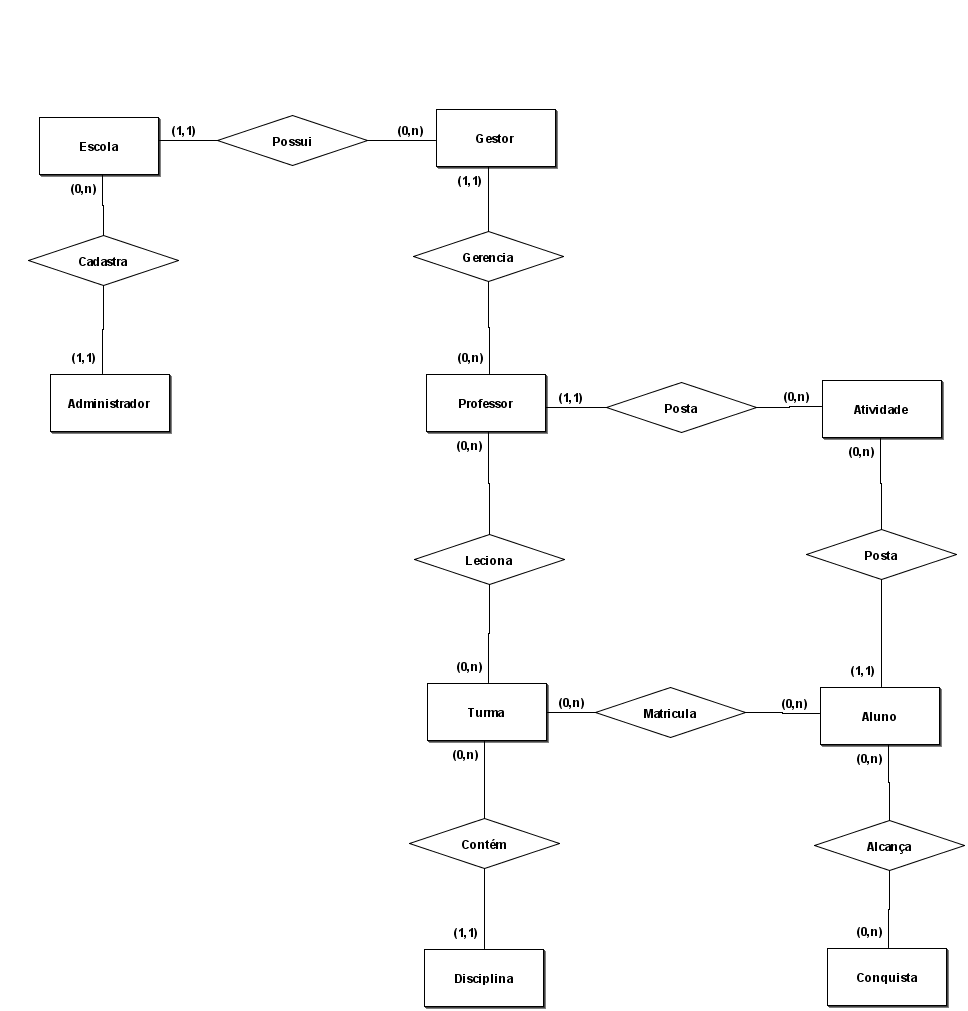
\includegraphics[width=16cm]{DER.png}
	\caption{\label{recompensa} Diagrama de Entidade Relacionamento}
	\fonte{Os autores}
\end{figure}
\FloatBarrier


\chapter{Viabilidade financeira}
O fato da aplicação ser \textit{open source} restringe a possibilidade de se ganhar dinheiro com venda direta, porém possibilita obtenção de lucro por meio de outras formas, como por exemplo:

\begin{itemize}
   \item \textbf{Utilização do servidor do fornecedor}: Nessa ocasião, a empresa contratante pagará um aluguel mensal para utilizar a aplicação hospedada no servidor do fornecedor.
   \item \textbf{Utilização de servidor próprio}: Utilização da aplicação em um servidor próprio da empresa contratante via pagamento de uma taxa de implementação mais uma de manutenção. Apesar de pagar mais pela implementação em um servidor próprio, a empresa contratante terá o direito de personalizar o produto de acordo com suas preferências nesse método de cobrança.
\end{itemize}

Há ainda a possibilidade de compilação independente do código-fonte da aplicação, por conta da premissa \textit{open source} citada anteriormente. Nesses casos, o fornecedor não se responsabilizará pela prestação de suporte.


Como forma de manter a aplicação, será cobrada uma taxa de R\$10,00 de cada aluno (sendo pago por ele ou pelo mantenedor da instituição de ensino) para que seu acesso à aplicação seja concedido. Desse modo, os custos com hospedagem já estariam cobertos a longo prazo, conforme a tabela abaixo:

\ABNTEXfontereduzida
\begin{table}[htb]
\centering
\caption{Previsão orçamentária mensal do Projeto Turma de Elite}
\label{tab-exemplo}
\begin{tabular}{|p{2.5cm}|c|c|c|c|c|}
   \hline
   \thead{} & \thead{100 alunos}  & \thead{1000 alunos}  & \thead{5000 alunos} & \thead{10000 alunos} & \thead{50000 alunos} \\\hline
   Heroku & R\$127* & R\$506* & R\$1010* & R\$5048* & R\$10096*  \\\hline
    Firebase Hosting & R\$0 & R\$177* & R\$411* & R\$832* & R\$5689* \\\hline
    Firebase Authentication & R\$0 & R\$0 & R\$0 & R\$3029* & R\$18172* \\\hline
    Receita & R\$1000 & R\$10000 & R\$50000 & R\$100000 & R\$500000 \\\hline
    Lucro & R\$873 & R\$9317 & R\$48579 & R\$91091 & R\$466043\\\hline
\end{tabular}
\fonte{Dados do Projeto}
\end{table}

Com relação aos \textit{dynos} do \textit{Heroku} para hospedar a quantidade crescente de acessos concorrentes, a relação obtida foi:
\begin{itemize}
    \item \textbf{100 alunos}: 1 \textit{dyno} - \textit{Standard} 1X
    \item \textbf{1000 alunos}: 2 \textit{dynos} - Standard 1X
    \item \textbf{5000 alunos}: 4 \textit{dynos} - Standard 2X
    \item \textbf{10000 alunos}: 4 \textit{dynos} - Performance M
    \item \textbf{50000 alunos}: 2 \textit{dynos} - Performance L
\end{itemize}

O custo de hospedagem e autenticação variou conforme a quantidade de armazenamento e suporte a acessos simultâneos necessários para atender a quantidade crescente de alunos.
% ---


% exemplos de escrita LaTeX e erros comuns
%\chapter{Exemplos \LaTeX}
\label{cap-exemplos}

\explicacao{ATENÇÃO : Este capítulo e os seguintes demonstram como fazer no \LaTeX portanto devem ser lidos em conjunto com o código fonte desse documento}

% exemplo de como inserir uma referencia adicional no sumario (normalmente não utilizado em um trabalho acadêmico)
\addcontentsline{toc}{chapter}{Exemplos que devem ser lidos (mas esse tipo de indicação não vai em um trabalho acadêmico) :-)}

Esse capítulo tem exemplos de escrita utilizando o \LaTeX  utilizando \abnTeX, é muito simples escrever em \textbf{negrito}, \emph{itálico}, ....


Existem diversos tutoriais para uso de \LaTeX, se você está utilizando esse modelo não precisará se preocupar com muitos dos detalhes técnicos do \LaTeX \space e cuidar somente do seu texto.

Escolha seu editor : \url{https://en.wikipedia.org/wiki/Comparison\_of\_TeX\_editors}, apesar do overleaf sem bem prático, nem todas as funções estão disponíveis na versão gratuita e você pode instalar gratuitamente em seu computador um compilador \LaTeX \space e utilizar um sistema de controle de versão para gerenciar seu documento.


\section{Normas ABNT}

Leia os documentos do \abnTeX e do \ac{ifsp}:
\begin{itemize}
    \item \url{http://www.abntex.net.br/}
    
    \item \acs{faq} : \url{https://github.com/abntex/abntex2/wiki/FAQ}
    
    \item \url{http://mirror.unl.edu/ctan/macros/latex/contrib/abntex2/doc/abntex2.pdf}
    
    \item \waUrl{https://spo.ifsp.edu.br/biblioteca?id=184}
\end{itemize}

No \ac{ifsp} você pode acessar todas as normas \ac{abnt} sem custo, as informações estão disponíveis no endereço \waUrl{http://www.ifsp.edu.br/index.php/outras-noticias/52-reitoria/2329-alunos-e-servidores-do-ifsp-podem-acessar-abnt-via-web.html}



\section{Detalhes textuais}

O documento é dividido em capítulos, e cada capítulo dividido em seções utilizando o \abnTeX \space você pode dividir seus documentos nos níveis a seguir:

\begin{itemize}
\item chapter (1);
\item section (1.1);
\item subsection (1.1.1);
\item subsubsection (1.1.1.1);
\item subsubsubsection (1.1.1.1.1).
\end{itemize}

Tenha em mente que normalmente se utiliza no máximo o nível \emph{subsection}.
Ao definir as divisões do seu trabalho utilizando as diretivas do \LaTeX, elas são automaticamente inseridas no sumário do documento.


\subsection{Caracteres Reservados e auxiliares}



Alguns caracteres são reservados no \LaTeX \space e por isso para utilizar esses caracteres é necessário utilizar uma forma diferenciada de escrita. É possível utilizar a macro \emph{symbol} com o código \ac{ascii} do caracter desejado, veja no código fonte desse texto como utilizar corretamente esses itens.


\begin{itemize}
\item barra invertida : \textbackslash   \symbol{92}    $\backslash$;
\item til  :  \symbol{126} ;
\item cifrão : \$;
\item sublinhado, \emph{underscore}, \emph{underline} : \_;
\item \enquote{aspas} as macros \emph{enquote} / \emph{textquote} garantem o espaçamento correto, se utilizar diretamente as ASPAS o espaçamento é perdido;
% https://tex.stackexchange.com/questions/80395/no-space-after-closing-double-quote
\item marcadores : \cmark\ \xmark\ \circlemark\ \ding{100} \ - ver mais no \refanexo{pifont-quickref};
\item chaves : \} \{.
\end{itemize}

\subsection{Listas}

Em uma lista de itens cada item deve ser terminado por ponto e virgula, exceto o ultimo item que deve ter um ponto final.

\begin{itemize}
\item item 1;
\item item 2;
\item item ..;
\item item final.
\end{itemize}


\subsection{Citações / Referências}
\label{referencias}

Existem diversas formas de citação observe os exemplos :

\begin{itemize}
    \item \cite{UML:JACOBSON} | \cite{POWELL:2006} \\ 
        \cite{SCRUMGUIDE:2013} | \cite{urani1994} |\\
        \cite{ETAL5} | \cite{ETAL4}; 
    
    \todo[inline]{Se as duas ultimas referencias aparecem somente com um autor, você está compilando o documento com uma versão antiga do \emph{abntexcite}, o overleaf em 2020-01-06 estava desatualizado}

    \item \citeonline{UML:JACOBSON} | \citeonline{POWELL:2006} \\
        \citeonline{SCRUMGUIDE:2013} | \citeonline{urani1994} | \\
        \citeonline{ETAL5} | \citeonline{ETAL4};

    \item \citeauthoronline{UML:JACOBSON}| \citeauthoronline{POWELL:2006} \\
        \citeauthoronline{SCRUMGUIDE:2013} | \citeauthoronline{urani1994} | \\
        \citeauthoronline{ETAL5} | \citeauthoronline{ETAL4};

    \item \citeauthor{UML:JACOBSON}| \citeauthor{POWELL:2006} \\
        \citeauthor{SCRUMGUIDE:2013}| \citeauthor{urani1994} | \\
        \citeauthor{ETAL5} | \citeauthor{ETAL4};
    
    \todo[inline]{Se as duas ultimas referencias aparecem somente com um autor, você está compilando o documento com uma versão antiga do \emph{abntexcite}, o overleaf em 2020-01-06 estava desatualizado}
    
\end{itemize}

A documentação do abntex2cite possui muitos exemplos de como utilizar corretamente cada formato de citação : \url{http://mirrors.ibiblio.org/CTAN/macros/latex/contrib/abntex2/doc/abntex2cite-alf.pdf}.

Cada formato de citação deve ser utilizado em um contexto especifico :
\begin{itemize}
    \item De acordo com \citeonline{SCRUMGUIDE:2013} .....;
    
    \item Fonte: \citeonline{SCRUMGUIDE:2013};
    
    \item sua explicação de um assunto baseado em uma referência \cite{SCRUMGUIDE:2013}.
    
\end{itemize}

ATENÇÃO : Alguns parâmetros de formatação foram alterados em 2018, mas não foram corrigidos ainda nos pacotes do \ac{abntex}, devem ser alterados manualmente ou utilizar as versões de desenvolvimento
\begin{itemize}
    \item \url{https://github.com/abntex/abntex2/issues/210}
    
    \item \url{https://github.com/abntex/biblatex-abnt/issues/42}
\end{itemize}

Os dados devem ser definidos corretamente nos arquivos \textquote{.bib} para a correta formatação no texto e na lista de referências.

Autor com diversas publicações no mesmo ano : são geradas letras automaticamente pelo compilador de acordo com a ordem que são apresentadas na bibliografia, a letra não aparece na lista de referencias. \footnote{\url{https://github.com/abntex/biblatex-abnt/issues/20}}


\subsection{Abreviaturas / Siglas / Glossário}
\label{siglas-glossario}

Palavras que devem ser apresentadas no glossário devem ser citadas especificamente no texto utilizando os comandos de glossário como : \gls{tag}.

Abreviaturas podem ser referenciadas diretamente na versão reduzida \textquote{\acs{ifsp}} \space  
ou longa \textquote{\acl{ifsp}}.

Na primeira vez que a sigla aparecer no texto o compilador mostra por extenso e a partir dai mostra somente a sigla:

\begin{itemize}
    \item \gls{se}
    \item \gls{se}
\end{itemize}

Lembre que o \LaTeX \ tem vários passos de compilação, sempre que alterar as chamadas de siglas / referencias é recomendável uma compilação completa.








\subsection{Elementos não textuais / Ilustrações}
\label{elementos-nao-textuais}

Elementos não textuais são aqueles que auxiliam o entendimento, não podem ficar \enquote{jogados} no texto, devem ser citados, cada elemento deve ser identificado por um \emph{label} único que permite a sua referencia, no texto utilizando \emph{ref} ou \emph{autoref}, esses elementos quando definidos corretamente também são inseridos nas listas presentes antes do sumário.

Cuidado com o artigo \textbf{O/A} antes da Figura, Tabela ou Quadro referenciado, deve ser compatível com o tipo da ilustração.

Lembre que o \LaTeX \  vai posicionar os elementos  da melhor maneira possível dentro do documento, sempre faça as referencias utilizando os comandos específicos, nunca utiliza \enquote{acima}, \enquote{"baixo}, \enquote{a seguir}, etc... 

O posicionamento desses elementos é feito pelas rotinas do pacote float, leia a documentação em  \url{http://linorg.usp.br/CTAN/macros/latex/contrib/float/float.pdf}. É recomendável utilizar as opções de posicionamento \textbf{htb}, a opção \textbf{H} deverá ser utilizada somente como ultima alternativa de posicionamento e em alguns casos a utilização de \textbf{$\backslash$FloatBarrier} pode também melhorar o resultado se utilizada com cuidado.


Para casos onde existe uma grande distancia entre a ilustração e o ponto de referencia no texto esse modelo possui macros \emph{autorefwithpage} e \emph{autorefwithpagedistance} a primeira sempre indica página onde a ilustração foi colocada e a segunda somente se a ilustração estiver mais distante que o número de páginas indicado como parâmetro, Ex. \autorefwithpage{fig_logo_A3}. Isso deve ser utilizado somente quando existe mais de uma referencia para mesma ilustração e não para deixar a ilustração distante de uma única referencia.





% ---
\subsection{QR-Code}
% ---
\index{qr-code}
A utilização de códigos \ac{qr} facilita o acesso de endereços da internet a partir de dispositivos móveis com câmera.
As figuras \ref{qr-url-1} e \ref{qr-url-2} demonstram dois exemplos de endereços apresentados com essa tecnologia.


Para facilitar a utilização dos códigos \ac{qr}, deve-se tomar cuidado para não deixa-los alinhados na vertical se houverem vários seguidos, pois dificulta a seleção a partir da câmera no dispositivo móvel.

Um exemplo para utilização de mais códigos de barra pode ser visto em : \urlmodelo.

Atenção, alguns compiladores podem ter problemas em utilizar a biblioteca \textbf{pstricks} necessária para gerar QR-Codes, no sharelatex em 2017-05 a compilação ocorre perfeitamente utilizando a opção de compilador "XeLatex", ele é mais lento que outras opções.


\begin{figure}[htb]
\begin{pspicture}(25mm,25mm)
\psbarcode{\urlmodelosimples}{eclevel=H width=1.0 height=1.0}{qrcode}
\end{pspicture}
\caption{\label{qr-url-1}QR-Code - URL Documento exemplo}
\legend{\urlmodelo}
\fonte{Os Autores}
\end{figure}



% colocando figura qrcode na direita para facilitar o uso da camera deixando cada qrcode em um alinhamento diferente
% se deixar os dois qrcodes um em cima do outro dificulta acessar o desejado
\begin{figure}[htb]
\begin{flushright}
\begin{pspicture}(25mm,25mm)
\psbarcode{https://github.com/ivanfmartinez/latexlib/tree/master/ifsp}{eclevel=H width=1.0 height=1.0}{qrcode}
\end{pspicture}
\caption{\label{qr-url-2}QR-Code - Classes IFSP GitHub}
\legend{\url{https://github.com/ivanfmartinez/latexlib/tree/master/ifsp}}
\fonte{Os Autores}
\end{flushright}

\end{figure}


\subsection{Organizando pendências}

Durante o desenvolvimento de um trabalho escrito é normal que alguns elementos sejam gerados posteriormente, mas é importante se organizar para não esquecer de fazer os ajustes necessários. Para isso recomendo a utilização do pacote \textbf{todonotes} que oferece diversos recursos para gerar lembretes das pendencias. O manual do \textbf{todonotes} está disponível no \autoref{manual-todonotes}\footnote{existe um bug no abntex2 ao referenciar anexos para fazer corretamente veja \url{https://github.com/abntex/abntex2/issues/76}}.

É possível fazer anotações de pendencias inclusive indicando as pessoas responsáveis por elas, % nao mover o todo o texto utiliza como exemplo indicando  fica assim errado
\todo[inline,author=Pessoa1]{fazer revisão das imagens do texto} e para facilitar a visualização criar imagens que funcionam como marcadores para figuras que serão incluídas posteriormente.

Cuidado ao utilizar as anotações \emph{inline} pois o texto ficara quebrado, como no paragrafo anterior.


\begin{figure}[htb]
    \centering
	\missingfigure[figwidth=10cm]{você está atrasado pois ainda não criou esta figura}
	\caption{\label{fig_todo1}Imagem que ainda não foi gerada}
	\fonte{dados do Projeto}
\end{figure}



\subsection{Tabelas e Quadros}
\label{tabelas-e-quadros}
A ‘norma’ 14724 \cite[3.32]{NBR14724:2011} define a Tabela como sendo uma \enquote{forma não discursiva de apresentar informações das quais o dado numérico se destaca como informação central}.

Quadros e tabelas são informações tabulares, mas Tabelas tem como objetivo apresentar números.

Uso de tabelas no \LaTeX : \url{https://en.wikibooks.org/wiki/LaTeX/Tables}

\textbf{Antes de utilizar \index{longtable}longtable procure reorganizar o seu layout ou quebrar manualmente em múltiplos quadros / tabelas, pois isso ainda facilita a compreensão pelo leitor.}



\index{quadros}O \autoref{quadro-exemplo} é um exemplo de dados tabulares gerados em 
\LaTeX.



\begin{quadro}[htb]
\centering
\ABNTEXfontereduzida
\caption[Níveis de investigação]{Níveis de investigação.}
\label{quadro-exemplo}
\begin{tabular}{|p{2.6cm}|p{6.0cm}|p{2.25cm}|p{3.40cm}|}
  \hline
   \thead{Nível de\\Investigação} & \thead{Insumos}  & \thead{Sistemas de\\ Investigação}  & \thead{Produtos}  \\
    \hline
    Meta-nível & Filosofia\index{filosofia} da Ciência  & Epistemologia &
    Paradigma  \\
    \hline
    Nível do objeto & Paradigmas do metanível e evidências do nível inferior &
    Ciência  & Teorias e modelos \\
    \hline
    Nível inferior & Modelos e métodos do nível do objeto e problemas do nível inferior & Prática & Solução de problemas  \\
   \hline
\end{tabular}
\legend{Fonte: Próprio Autor}
\end{quadro}



\index{tabelas}Já a \autoref{tab-exemplo} foi criada conforme o padrão do \ac{ibge}
requerido pelas normas da \ac{abnt} para documentos técnicos e acadêmicos. Observe que não existem bordas laterais em uma Tabela e as colunas numéricas tem alinhamento à direita.

\begin{table}[htb]
\centering
\caption{Um Exemplo de tabela}
\label{tab-exemplo}
\begin{tabular}{p{2.6cm}|r|r|r}
    \hline
   \thead{Item} & \thead{Janeiro}  & \thead{Fevereiro}  & \thead{Março}  \\
    \hline
    Classes & 2  & 10 & 20  \\
    \hline
    Linhas & 100  & 250 & 543 \\
    \hline
\end{tabular}
\fonte{Dados do Projeto}
\end{table}

\def\equationautorefname~#1\null{%
  Equação~(#1)\null
}


Para facilitar a criação de tabelas e quadros existem algumas ferramentas como o Tables Generator \url{http://www.tablesgenerator.com/latex_tables} que permite a criação de forma visual gerando o código \LaTeX\ correspondente. E o site \url{https://www.latex-tables.com/} permite converter planilhas em código \LaTeX.


\index{equação}\index{Pitágoras}A \autoref{eq-pythagoras} demonstra que também é possível escrever equações diretamente em \LaTeX

\begin{equation}\label{eq-pythagoras}
a^2+b^2=c^2\,.
\end{equation}






% ---
\subsection{Figuras}
\label{sec_figuras}
% ---

\index{figuras}Figuras podem ser criadas diretamente em \LaTeX,
como o exemplo da \autoref{fig_circulo}, ou inseridas a partir de arquivos externos como a \autoref{fig_logo}, que é o Logotipo do \ac{ifsp}. \index{logotipo}

As figuras externas devem possuir boa qualidade e preferencialmente serem vetorizadas para se obter o melhor resultado. A \autoref{fig:nao_vetorizado_e_vetorizado} apresenta duas versões de uma mesma imagem demonstrando a variação de qualidade que pode acontecer quando não for utilizada a versão vetorizada, quando a figura possui elementos textuais pode até inviabilizar a leitura. As Figuras \ref{fig:uml_dia_nao_vetorizado_jpeg}, \ref{fig:uml_dia_vetorizado_eps} e \ref{fig:uml_dia_vetorizado_svg} foram reduzidas propositalmente no documento para demonstrar a diferença entre os formatos de arquivo. A diferença fica mais perceptível quando o documento é impresso ou quando existem textos pequenos e é necessário fazer zoom para visualização.

Procure criar suas imagens e diagramas pensando em utilizar impressão em preto-e-branco ou escala de cinza. Isto é importante, principalmente quando se pretende publicar o trabalho, uma vez que a maioria das publicações são somente em preto-e-branco. Outro benefício é o custo de impressão, normalmente menor para páginas preto-e-branco em relação a páginas coloridas.

Para diagramas em \ac{uml} o PlantUML pode ser utilizado para gerar código {\LaTeX} como exemplo na  \autoref{diagramauml}.


Se não houver a possibilidade de utilização de uma imagem vetorizada e existem diversos detalhes utilize \ac{png} em vez de JPG \footnote{Abreviado de \ac{jpeg}}, observe a diferença no exemplo em \waUrl{https://tex.stackexchange.com/questions/136087/selecting-best-file-extension-for-graphics-figures-pictures}.


\begin{figure}[htb]
	\begin{center}
	    \setlength{\unitlength}{5cm}
		\begin{picture}(1,1)
		\put(0,0){\line(0,1){1}}
		\put(0,0){\line(1,0){1}}
		\put(0,0){\line(1,1){1}}
		\put(0,0){\line(1,2){.5}}
		\put(0,0){\line(1,3){.3333}}
		\put(0,0){\line(1,4){.25}}
		\put(0,0){\line(1,5){.2}}
		\put(0,0){\line(1,6){.1667}}
		\put(0,0){\line(2,1){1}}
		\put(0,0){\line(2,3){.6667}}
		\put(0,0){\line(2,5){.4}}
		\put(0,0){\line(3,1){1}}
		\put(0,0){\line(3,2){1}}
		\put(0,0){\line(3,4){.75}}
		\put(0,0){\line(3,5){.6}}
		\put(0,0){\line(4,1){1}}
		\put(0,0){\line(4,3){1}}
		\put(0,0){\line(4,5){.8}}
		\put(0,0){\line(5,1){1}}
		\put(0,0){\line(5,2){1}}
		\put(0,0){\line(5,3){1}}
		\put(0,0){\line(5,4){1}}
		\put(0,0){\line(5,6){.8333}}
		\put(0,0){\line(6,1){1}}
		\put(0,0){\line(6,5){1}}
		\end{picture}
	\end{center}
	\caption{\label{fig_circulo}A delimitação do espaço}
	\fonte{Modelo Canônico ABNTeX2}
\end{figure}


\begin{figure}[htb]
    \centering
	
\includegraphics{\ifspprefixo/logo-02.jpg}
	\caption{\label{fig_logo}Logotipo \ac{ifsp}}
	\fonte{\ac{ifsp}}
\end{figure}

\begin{figure}
    \centering
	
\includegraphics[width=0.95\textwidth]{erros/exemploVetorizacao.png}
    \caption{Exemplo de imagem não vetorizada e vetorizada}
    \label{fig:nao_vetorizado_e_vetorizado}
    \fonte{\citeonline{vetorizacao}}
\end{figure}
    

% Essas imagens foram reduzidas na apresentação para demonstrar o efeito da alteração de escala em imagens não vetorizadas
\begin{figure}
    \centering
	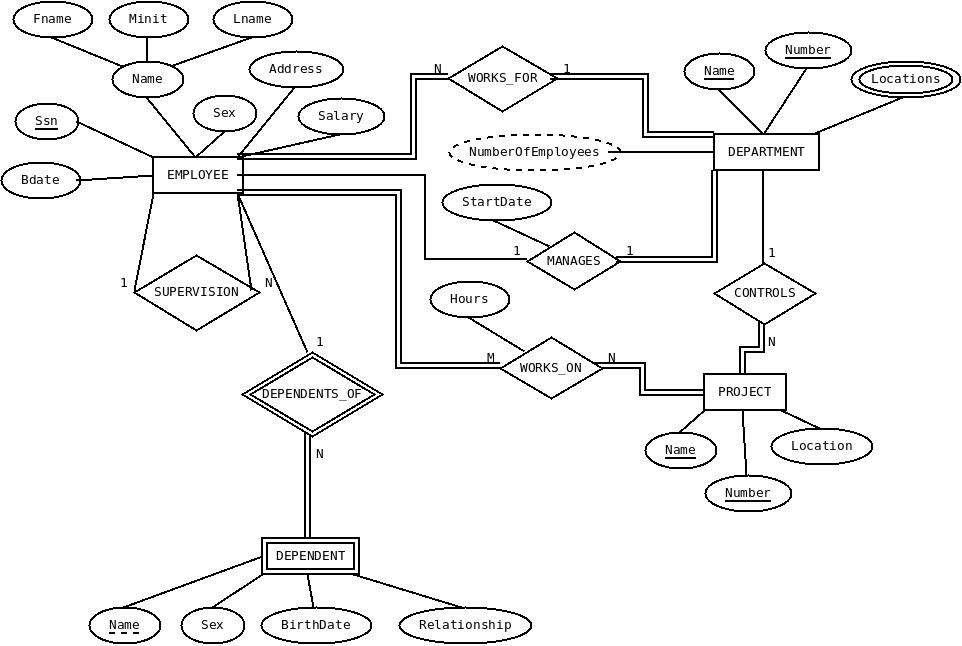
\includegraphics[width=0.6\textwidth]{exemplos/diagramas/ER.jpeg}
    \caption{Exemplo de diagrama - salvo em imagem não vetorizada - JPEG}
    \label{fig:uml_dia_nao_vetorizado_jpeg}
\end{figure}


\begin{figure}
    \centering
	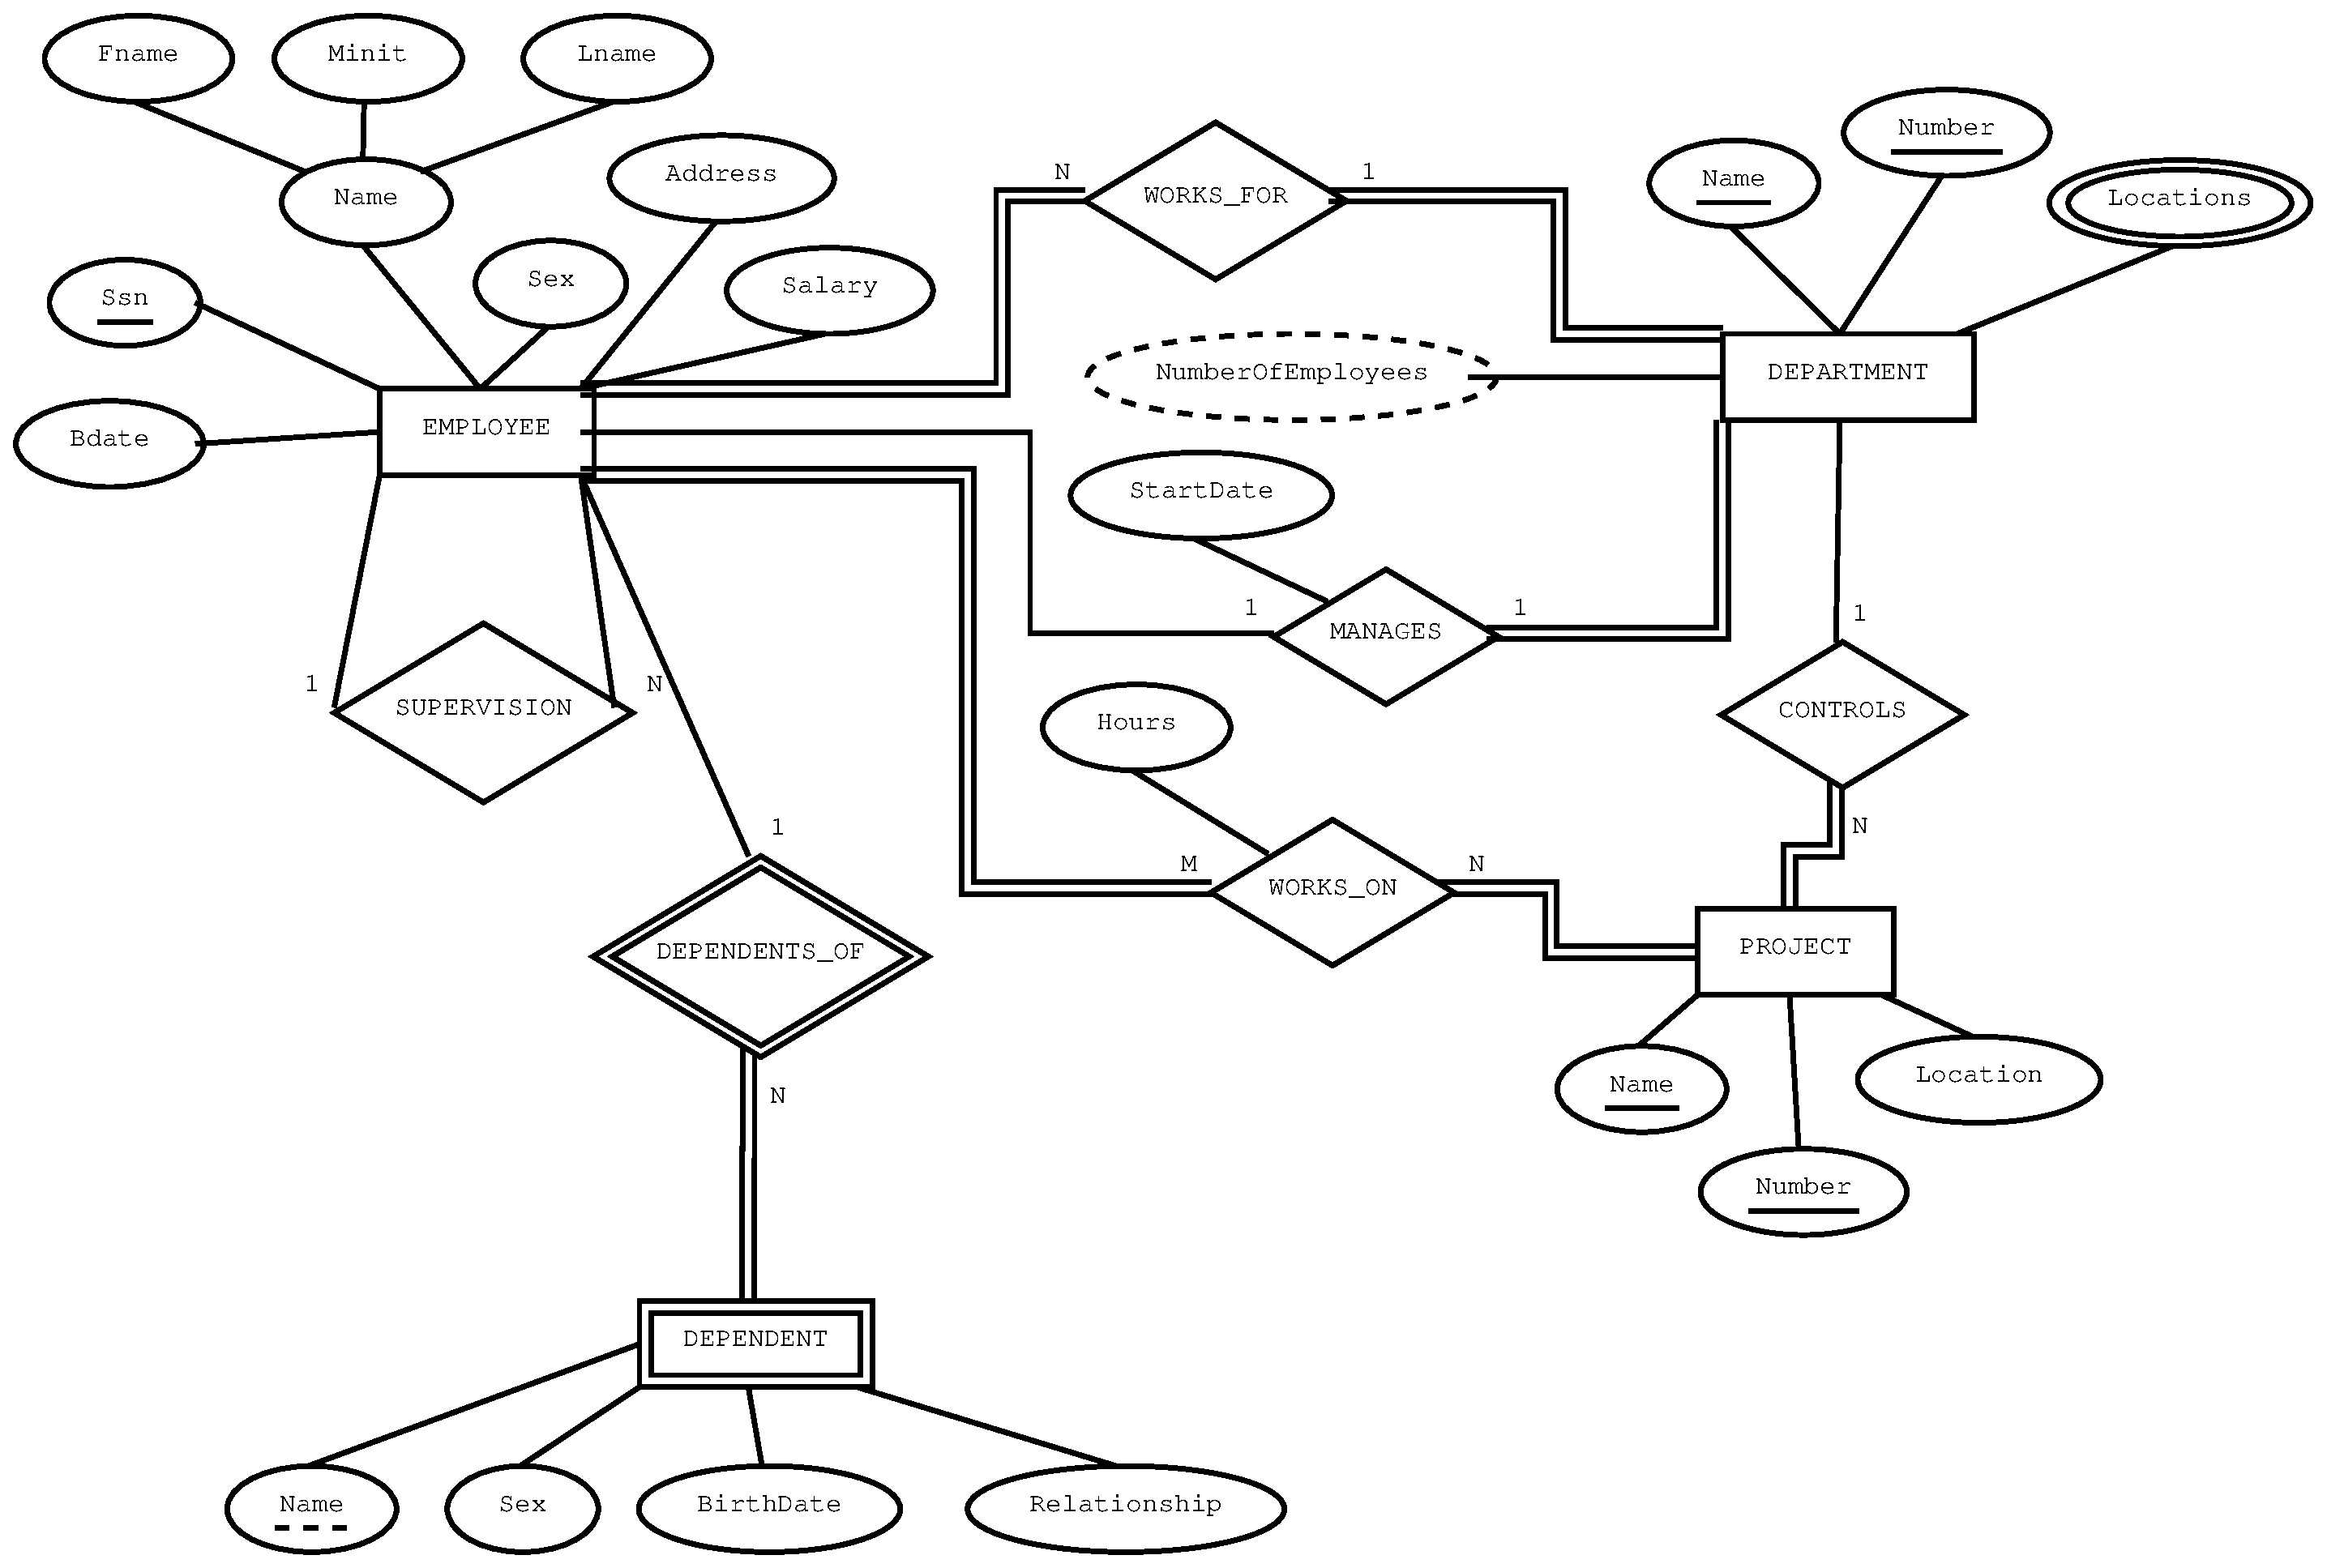
\includegraphics[width=0.6\textwidth]{exemplos/diagramas/ER.eps}
    \caption{Exemplo de diagrama - salvo imagem vetorizada - EPS}
    \label{fig:uml_dia_vetorizado_eps}
\end{figure}

\begin{figure}
    \centering
	\includesvg[inkscapelatex=false,width=0.6\textwidth]{exemplos/diagramas/ER.svg}
    \caption{Exemplo de diagrama - salvo imagem vetorizada - SVG}
    \label{fig:uml_dia_vetorizado_svg}
\end{figure}



% generated by Plantuml 7997beta
\definecolor{plantucolor0000}{RGB}{254,254,206}
\definecolor{plantucolor0001}{RGB}{168,0,54}
\definecolor{plantucolor0002}{RGB}{173,209,178}
\definecolor{plantucolor0003}{RGB}{0,0,0}
\definecolor{plantucolor0004}{RGB}{0,0,255}

\begin{figure}[htb]
    \centering
\begin{tikzpicture}[yscale=-1]
\draw[color=plantucolor0001,fill=plantucolor0000,line width=1.5pt] (131pt,29pt) rectangle (223pt,90.8359pt);
\draw[color=plantucolor0001,fill=plantucolor0002,line width=1.0pt] (146pt,45pt) ellipse (11pt and 11pt);
\draw[color=black,fill=black] (148.7656pt,40.875pt) ..controls (148.9219pt,40.6563pt) .. (149.1094pt,40.5469pt) ..controls (149.2969pt,40.4375pt) .. (149.5156pt,40.4375pt) ..controls (149.8906pt,40.4375pt) .. (150.125pt,40.6953pt) ..controls (150.3594pt,40.9531pt) .. (150.3594pt,41.5625pt) -- (150.3594pt,43.0156pt) ..controls (150.3594pt,43.625pt) .. (150.125pt,43.8906pt) ..controls (149.8906pt,44.1563pt) .. (149.5156pt,44.1563pt) ..controls (149.1719pt,44.1563pt) .. (148.9688pt,43.9531pt) ..controls (148.7656pt,43.7656pt) .. (148.6563pt,43.25pt) ..controls (148.6094pt,42.8906pt) .. (148.4219pt,42.7031pt) ..controls (148.0938pt,42.3281pt) .. (147.4844pt,42.1094pt) ..controls (146.875pt,41.8906pt) .. (146.25pt,41.8906pt) ..controls (145.4844pt,41.8906pt) .. (144.8516pt,42.2188pt) ..controls (144.2188pt,42.5469pt) .. (143.7266pt,43.2969pt) ..controls (143.2344pt,44.0469pt) .. (143.2344pt,45.0781pt) -- (143.2344pt,46.1719pt) ..controls (143.2344pt,47.4063pt) .. (144.125pt,48.2266pt) ..controls (145.0156pt,49.0469pt) .. (146.6094pt,49.0469pt) ..controls (147.5469pt,49.0469pt) .. (148.2031pt,48.7969pt) ..controls (148.5938pt,48.6406pt) .. (149.0156pt,48.2031pt) ..controls (149.2813pt,47.9375pt) .. (149.4297pt,47.8594pt) ..controls (149.5781pt,47.7813pt) .. (149.7813pt,47.7813pt) ..controls (150.1094pt,47.7813pt) .. (150.3672pt,48.0391pt) ..controls (150.625pt,48.2969pt) .. (150.625pt,48.6406pt) ..controls (150.625pt,48.9844pt) .. (150.2813pt,49.3906pt) ..controls (149.7813pt,49.9688pt) .. (148.9844pt,50.2969pt) ..controls (147.9063pt,50.75pt) .. (146.6094pt,50.75pt) ..controls (145.0938pt,50.75pt) .. (143.8906pt,50.125pt) ..controls (142.9063pt,49.625pt) .. (142.2188pt,48.5547pt) ..controls (141.5313pt,47.4844pt) .. (141.5313pt,46.2031pt) -- (141.5313pt,45.0469pt) ..controls (141.5313pt,43.7188pt) .. (142.1484pt,42.5703pt) ..controls (142.7656pt,41.4219pt) .. (143.8594pt,40.8047pt) ..controls (144.9531pt,40.1875pt) .. (146.1875pt,40.1875pt) ..controls (146.9219pt,40.1875pt) .. (147.5703pt,40.3516pt) ..controls (148.2188pt,40.5156pt) .. (148.7656pt,40.875pt);
\node at (160pt,37.4531pt)[below right]{Subscriber};
\draw[color=plantucolor0001,line width=1.5pt] (132pt,61pt) -- (222pt,61pt);
\node at (137pt,65pt)[below right]{subscriberId};
\draw[color=plantucolor0001,line width=1.5pt] (132pt,82.8359pt) -- (222pt,82.8359pt);
\draw[color=plantucolor0001,fill=plantucolor0000,line width=1.5pt] (31pt,212pt) rectangle (137pt,273.8359pt);
\draw[color=plantucolor0001,fill=plantucolor0002,line width=1.0pt] (46pt,228pt) ellipse (11pt and 11pt);
\draw[color=black,fill=black] (48.7656pt,223.875pt) ..controls (48.9219pt,223.6563pt) .. (49.1094pt,223.5469pt) ..controls (49.2969pt,223.4375pt) .. (49.5156pt,223.4375pt) ..controls (49.8906pt,223.4375pt) .. (50.125pt,223.6953pt) ..controls (50.3594pt,223.9531pt) .. (50.3594pt,224.5625pt) -- (50.3594pt,226.0156pt) ..controls (50.3594pt,226.625pt) .. (50.125pt,226.8906pt) ..controls (49.8906pt,227.1563pt) .. (49.5156pt,227.1563pt) ..controls (49.1719pt,227.1563pt) .. (48.9688pt,226.9531pt) ..controls (48.7656pt,226.7656pt) .. (48.6563pt,226.25pt) ..controls (48.6094pt,225.8906pt) .. (48.4219pt,225.7031pt) ..controls (48.0938pt,225.3281pt) .. (47.4844pt,225.1094pt) ..controls (46.875pt,224.8906pt) .. (46.25pt,224.8906pt) ..controls (45.4844pt,224.8906pt) .. (44.8516pt,225.2188pt) ..controls (44.2188pt,225.5469pt) .. (43.7266pt,226.2969pt) ..controls (43.2344pt,227.0469pt) .. (43.2344pt,228.0781pt) -- (43.2344pt,229.1719pt) ..controls (43.2344pt,230.4063pt) .. (44.125pt,231.2266pt) ..controls (45.0156pt,232.0469pt) .. (46.6094pt,232.0469pt) ..controls (47.5469pt,232.0469pt) .. (48.2031pt,231.7969pt) ..controls (48.5938pt,231.6406pt) .. (49.0156pt,231.2031pt) ..controls (49.2813pt,230.9375pt) .. (49.4297pt,230.8594pt) ..controls (49.5781pt,230.7813pt) .. (49.7813pt,230.7813pt) ..controls (50.1094pt,230.7813pt) .. (50.3672pt,231.0391pt) ..controls (50.625pt,231.2969pt) .. (50.625pt,231.6406pt) ..controls (50.625pt,231.9844pt) .. (50.2813pt,232.3906pt) ..controls (49.7813pt,232.9688pt) .. (48.9844pt,233.2969pt) ..controls (47.9063pt,233.75pt) .. (46.6094pt,233.75pt) ..controls (45.0938pt,233.75pt) .. (43.8906pt,233.125pt) ..controls (42.9063pt,232.625pt) .. (42.2188pt,231.5547pt) ..controls (41.5313pt,230.4844pt) .. (41.5313pt,229.2031pt) -- (41.5313pt,228.0469pt) ..controls (41.5313pt,226.7188pt) .. (42.1484pt,225.5703pt) ..controls (42.7656pt,224.4219pt) .. (43.8594pt,223.8047pt) ..controls (44.9531pt,223.1875pt) .. (46.1875pt,223.1875pt) ..controls (46.9219pt,223.1875pt) .. (47.5703pt,223.3516pt) ..controls (48.2188pt,223.5156pt) .. (48.7656pt,223.875pt);
\node at (60pt,220.4531pt)[below right]{AccumUsage};
\draw[color=plantucolor0001,line width=1.5pt] (32pt,244pt) -- (136pt,244pt);
\node at (37pt,248pt)[below right]{subscriberId};
\draw[color=plantucolor0001,line width=1.5pt] (32pt,265.8359pt) -- (136pt,265.8359pt);
\draw[color=plantucolor0001,fill=plantucolor0000,line width=1.5pt] (221pt,191pt) rectangle (318pt,294.3438pt);
\draw[color=plantucolor0001,fill=plantucolor0002,line width=1.0pt] (240.05pt,207pt) ellipse (11pt and 11pt);
\draw[color=black,fill=black] (242.8156pt,202.875pt) ..controls (242.9719pt,202.6563pt) .. (243.1594pt,202.5469pt) ..controls (243.3469pt,202.4375pt) .. (243.5656pt,202.4375pt) ..controls (243.9406pt,202.4375pt) .. (244.175pt,202.6953pt) ..controls (244.4094pt,202.9531pt) .. (244.4094pt,203.5625pt) -- (244.4094pt,205.0156pt) ..controls (244.4094pt,205.625pt) .. (244.175pt,205.8906pt) ..controls (243.9406pt,206.1563pt) .. (243.5656pt,206.1563pt) ..controls (243.2219pt,206.1563pt) .. (243.0188pt,205.9531pt) ..controls (242.8156pt,205.7656pt) .. (242.7063pt,205.25pt) ..controls (242.6594pt,204.8906pt) .. (242.4719pt,204.7031pt) ..controls (242.1438pt,204.3281pt) .. (241.5344pt,204.1094pt) ..controls (240.925pt,203.8906pt) .. (240.3pt,203.8906pt) ..controls (239.5344pt,203.8906pt) .. (238.9016pt,204.2188pt) ..controls (238.2688pt,204.5469pt) .. (237.7766pt,205.2969pt) ..controls (237.2844pt,206.0469pt) .. (237.2844pt,207.0781pt) -- (237.2844pt,208.1719pt) ..controls (237.2844pt,209.4063pt) .. (238.175pt,210.2266pt) ..controls (239.0656pt,211.0469pt) .. (240.6594pt,211.0469pt) ..controls (241.5969pt,211.0469pt) .. (242.2531pt,210.7969pt) ..controls (242.6438pt,210.6406pt) .. (243.0656pt,210.2031pt) ..controls (243.3313pt,209.9375pt) .. (243.4797pt,209.8594pt) ..controls (243.6281pt,209.7813pt) .. (243.8313pt,209.7813pt) ..controls (244.1594pt,209.7813pt) .. (244.4172pt,210.0391pt) ..controls (244.675pt,210.2969pt) .. (244.675pt,210.6406pt) ..controls (244.675pt,210.9844pt) .. (244.3313pt,211.3906pt) ..controls (243.8313pt,211.9688pt) .. (243.0344pt,212.2969pt) ..controls (241.9563pt,212.75pt) .. (240.6594pt,212.75pt) ..controls (239.1438pt,212.75pt) .. (237.9406pt,212.125pt) ..controls (236.9563pt,211.625pt) .. (236.2688pt,210.5547pt) ..controls (235.5813pt,209.4844pt) .. (235.5813pt,208.2031pt) -- (235.5813pt,207.0469pt) ..controls (235.5813pt,205.7188pt) .. (236.1984pt,204.5703pt) ..controls (236.8156pt,203.4219pt) .. (237.9094pt,202.8047pt) ..controls (239.0031pt,202.1875pt) .. (240.2375pt,202.1875pt) ..controls (240.9719pt,202.1875pt) .. (241.6203pt,202.3516pt) ..controls (242.2688pt,202.5156pt) .. (242.8156pt,202.875pt);
\node at (254.95pt,199.4531pt)[below right]{IpSession};
\draw[color=plantucolor0001,line width=1.5pt] (222pt,223pt) -- (317pt,223pt);
\node at (227pt,227pt)[below right]{ipAddress};
\node at (227pt,240.8359pt)[below right]{specificData};
\node at (227pt,254.6719pt)[below right]{sapcOriginStateId};
\node at (227pt,268.5078pt)[below right]{apnId};
\draw[color=plantucolor0001,line width=1.5pt] (222pt,286.3438pt) -- (317pt,286.3438pt);
\draw[color=plantucolor0004] (191.942pt,90.081pt) ..controls (205.204pt,115.893pt) and (224.952pt,154.325pt) .. (241.265pt,186.076pt);
\draw[color=plantucolor0004,fill=plantucolor0004] (243.646pt,190.709pt) -- (243.0894pt,180.8759pt) -- (241.3604pt,186.262pt) -- (235.9742pt,184.5329pt) -- (243.646pt,190.709pt) -- cycle;
\node at (191.0584pt,98.9168pt)[below right]{1};
\node at (230.3817pt,166.6703pt)[below right]{1..*};
\draw[color=plantucolor0001] (162.058pt,90.081pt) ..controls (145.645pt,122.023pt) and (119.302pt,173.295pt) .. (101.824pt,207.31pt);
\draw[color=plantucolor0001,fill=plantucolor0001] (99.5252pt,211.784pt) -- (107.1969pt,205.6078pt) -- (101.8108pt,207.337pt) -- (100.0816pt,201.9509pt) -- (99.5252pt,211.784pt) -- cycle;
\node at (143.0082pt,98.7264pt)[below right]{1};
\node at (101.801pt,187.522pt)[below right]{0..1};
\end{tikzpicture}
\caption{\label{diagramauml}Exemplo de Diagrama UML gerado a partir do PlantUML}
	\legend{Fonte: Exemplos PlantUML}
\end{figure}

A \autoref{fig_diag_virado} exemplifica como utilizar uma imagem em formato paisagem (página inteira). Obs: Utilizamos propositalmente uma imagem não vetorizada de forma a ilustrar o procedimento e também para apresentar que a qualidade não fica boa o suficiente para leitura. Uma versão vetorizada dessa figura teria qualidade melhor.


% observe que a imagem a seguir teve que ser ajustada para caber corretamente na página
% por não ser uma imagem vetorizada a qualidade não é a melhor possivel
\begin{sidewaysfigure}[htb]
    \centering
	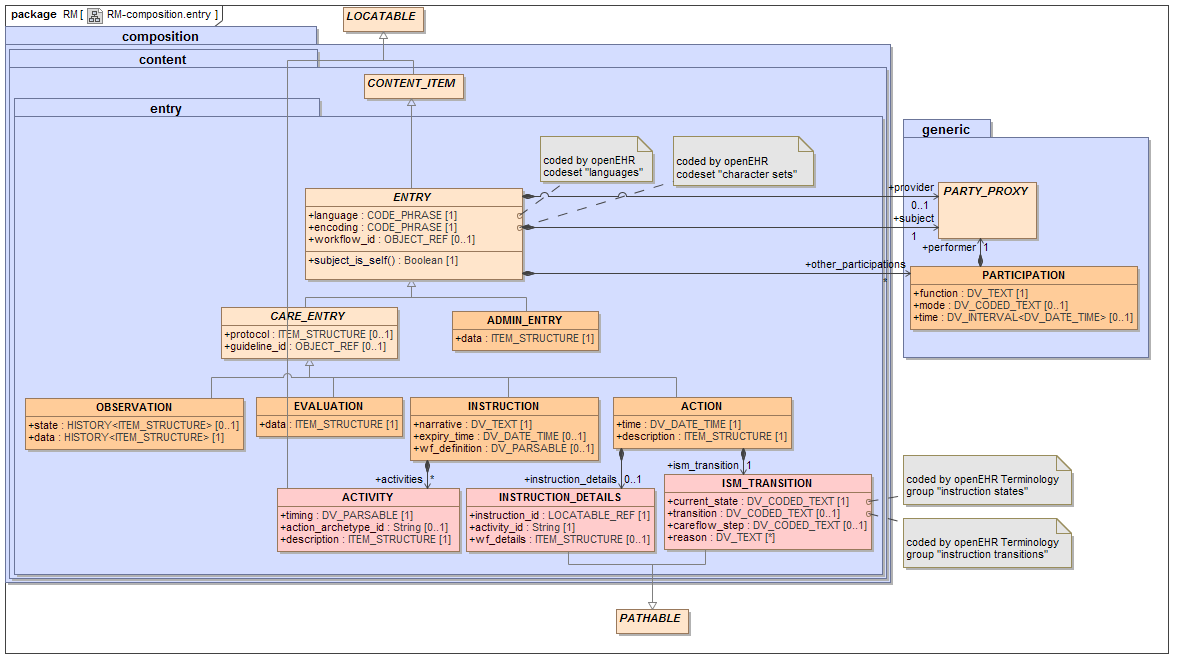
\includegraphics[width=0.9\textwidth]{exemplos/exemplo_diag_horizontal.png}
	\caption{\label{fig_diag_virado}Diagrama Virado - Exemplo}
	\fonte{\citeonline{openehrCompositionEntry}}
\end{sidewaysfigure}


\subsection{Impressão em folhas formato A3}

A página seguinte em A3 permite a impressão de diagramas grandes que não podem ser visualizados facilmente em folha padrão A4. Lembre que algumas impressoras podem ter problemas com isso, então selecione somente as páginas A4 ao imprimir e depois imprima separadamente a página A3.

A \autoref{fig_logo_A3} utiliza a mesma imagem da \autoref{fig_logo} e foi ampliada para demonstrar a essa possibilidade de impressão de grandes imagens em A3.

Observe que o código de exemplo vai gerar uma quebra de página no local onde for definida a página A3, por isso não deve ser utilizado entre textos para evitar grandes espaços em branco.

Folhas impressas em A3 ou tamanhos maiores devem ser dobradas seguindo o padrão definido pela ABNT. 


Cuidado ao utilizar folhas A3 em um documento impresso em frente e verso pois a numeração das páginas seguintes pode ser impressa de forma incorreta (posição do número na página). Uma alternativa para esta situação é manter todas páginas impressas em A3 no último apêndice, fazendo as referencias corretas durante o texto.



\afterpage{%
\begin{PAGINA-A3}

\begin{figure}[p]
    \centering%
    \fcolorbox{red}{yellow}{ 
\includegraphics[height=\textheight,width=\textwidth,keepaspectratio]{\ifspprefixo/logo-02.jpg}}%
	\caption{\label{fig_logo_A3}Logotipo IFSP em página A3}
	\legend{Com borda para demonstrar os limites}
   \fonte{Autor da Figura}
\end{figure}

\end{PAGINA-A3}
}


%%
% Macros para simplificar a demonstração dos erros
%

\newcommand{\errado}[1]{\textbf{\textcolor{red}{#1}}}
\newcommand{\certo}[1]{\textbf{\textcolor{ForestGreen}{#1}}}
% Para não confundir com os exemplos de certo e errado não são colocados os pontos e ponto e virgula dos itens
\newcommand{\erradocerto}[3]{\item #1:\begin{itemize}
    \item \errado{#2}
    \item \certo{#3}
\end{itemize}}
\newcommand{\erradoerradocerto}[4]{\item #1:\begin{itemize}
    \item \errado{#2}
    \item \errado{#3}
    \item \certo{#4}
\end{itemize}}



% Para demonstrar o erro nome deve ser igual entre o capitulo e a seção, então fica em um comando para facilitar
\newcommand{\nomeDoCapitulo}{Erros comuns em documentos}
\chapter{\nomeDoCapitulo}
\label{erros-comuns-capitulo}

% Não colocar nada aqui pois é uma demonstração de erro comum
\explicacaoErro{Passando de capítulo para seção sem texto}
\explicacaoErro{Seção com mesmo nome do capítulo}

\section{\nomeDoCapitulo}
\label{erros-comuns}

% Não colocar nada aqui pois é uma demonstração de erro comum
\explicacaoErro{Passando de seção para subseção sem texto}

\subsection{Subseção sem texto entre o item anterior}
\label{erros-comuns-sub1}


% Tem um erro proposital aqui duplicando "seção" que é escrita também pelo autoref....
Essa seção \autoref{erros-comuns} demonstra alguns dos erros mais comuns que percebemos em trabalhos de alunos. Alguns itens errados são apresentados em \errado{vermelho} e corretos em \certo{verde}, mas devido a formatação dos links pode haver uma variação.

Além desses erros é comum encontrar a falta de correção ortográfica e utilização errada de palavras. É importante sempre utilizar a correção ortográfica e ainda fazer a revisão por diversas pessoas para evitar erros de português, a língua portuguesa tem palavras parecidas com sentidos diferente, cuidado com a utilização dos acentos e pontuação como pode ser visto claramente em  \autoref{fig_portugues_amador}.

% erro proposital que esta no inicio da seção
Você percebeu que essa seção iniciou com um erro e que esse erro não está indicado em vermelho ?


\begin{figure}[htb]
    \centering
	\frame{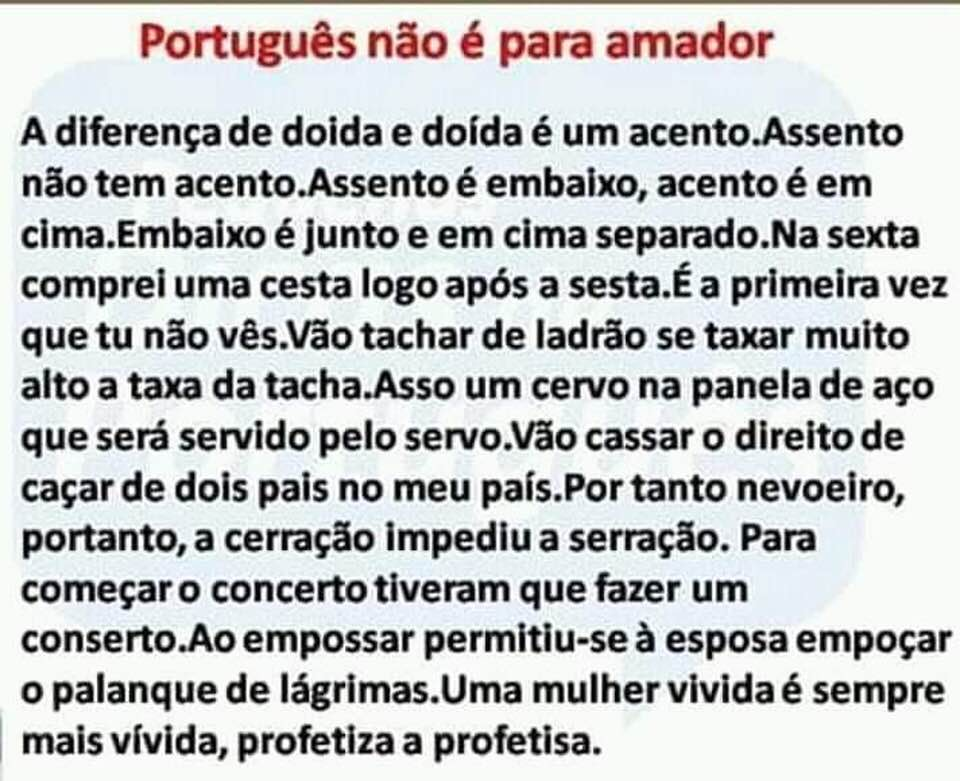
\includegraphics[width=0.9\textwidth]{erros/portugues_nao_eh_para_amador.jpg}}
	\caption{\label{fig_portugues_amador}Português não é para amador}
	\fonte{Autor Desconhecido}
\end{figure}


Exemplos de erros encontrados em documentos das disciplinas de projetos:
\todo[inline]{Separar esses itens em grupos mais específicos}


\begin{itemize}
    \item \errado{passagem de um item para outro sem texto} como é possível observar entre  \autoref{erros-comuns-capitulo} e \autoref{erros-comuns} e também entre \autoref{erros-comuns} e \autoref{erros-comuns-sub1};
    
    \item \errado{itens com pouco texto} como a \autoref{erros-comuns-sub-pequena1} e a \autoref{erros-comuns-sub-pequena2}, cada item deve ter um volume de texto que justifique sua existência;
        
    \item cada parágrafo deve descrever uma ideia então cuidado ao escrever um parágrafo grande demais com diversas ideias envolvidas; 
        
    \item \errado{utilizar o mesmo nome para seções / capítulos como \autoref{erros-comuns-capitulo} e \autoref{erros-comuns}};
        
    \item definições de referências incompletas, a referência \citeonline{ETAL4} está definida faltando cidade, observe que na lista de referencias aparece \errado{[S.l.]} que indica Sem Local, pois a \ac{abnt} exige a indicação de local para livros;
        
    \erradocerto{não utilizar o sistema de siglas / glossário para definições especificas,ver \autoref{siglas-glossario}}{IFSP}{\acs{ifsp}}
    
    \erradocerto{ignorar que após uma macro pode ser necessário incluir um espaço forçado}{o \LaTeX permite...}{o \LaTeX\ permite...}

    \erradocerto{não utilizar palavras em português onde for possível}{o dispositivo mobile}{o dispositivo móvel}

    \erradocerto{não utilizar melhores palavras, algumas palavras chegaram a ser incorporadas a língua portuguesa mas existem palavras melhores e que podem ser utilizadas e as vezes com resultado mais claro}{postagem / deletar}{publicação / excluir}

    \erradocerto{Utilização do tempo verbal incorreto, a escrita do documento muitas vezes inicia antes da finalização, mas o leitor recebe o documento depois do trabalho finalizado}{será desenvolvido - será apresentado}{foi desenvolvido - é apresentado}

    \erradocerto{não representar as unidades de forma correta}{3.20 ghz}{3.20 GHz}

    \erradocerto{não ser consistente com os formatos e precisões}{o primeiro tem \emph{clock} de 3.20 GHz e segundo 1.8 GHz}{o primeiro tem \emph{clock} de 3.20 GHz e segundo 1.80 GHz}

    \erradocerto{não referenciar ilustrações da forma correta}{a tabela \ref{tabela-correta-equipamento} ...}{a \autoref{tabela-correta-equipamento} ...}
    

    \erradocerto{não referenciar uma ilustração no texto, toda ilustração deve ser referenciada no texto}{(...)parecidas com sentidos diferente, cuidado com a utilização dos acentos e pontuação como pode ser visto abaixo.}{(...)parecidas com sentidos diferente, cuidado com a utilização dos acentos e pontuação como pode ser visto claramente em \autoref{fig_portugues_amador}}
    
    \erradocerto{não referenciar corretamente sequencias de ilustrações}{nas \autoref{tab-exemplo} até \autoref{tabela-correta-servicos}}{nas Tabelas de \ref{tab-exemplo} até \ref{tabela-correta-servicos}}

    \erradocerto{deixar referencia jogada sem fazer parte do texto}{durante o projeto foram registradas as métricas. \autoref{tabela-correta-servicos}}{a \autoref{tabela-correta-servicos} apresenta os valores das métricas levantadas durante o projeto.}

    \erradocerto{incluir dentro do seu texto um documento ou manual que pode ser referenciado e facilmente acessado pelo leitor,faça a citação correta referenciando o documento original}{segundo a LDB, a educação brasileira é dividida em dois níveis: a educação básica e o ensino superior}{segundo a LDB 9394/96 \cite{ldb}, a educação brasileira é dividida em dois níveis: a educação básica e o ensino superior}
    
    \erradocerto{citação de elementos errados}{Segundo o anexo com o manual pdfpages (\autoref{manual-todonotes}), o comando {\textbackslash}includepdf permite que você faça a inclusão de páginas de documentos externos no seu documento}{Segundo o anexo com o manual pdfpages (\autoref{manual-pdfpages}), o comando {\textbackslash}includepdf permite que você faça a inclusão de páginas de documentos externos no seu documento}
    
    
    \erradocerto{Escrever as mesmas palavras, com o mesmo sentido de diversas formas diferentes. Um exemplo é o nome de uma empresa famosa em alguns desenhos: ACME}{ACME Corporation é uma sociedade fictícia que existe no universo dos filmes e animações \newline ... \newline A companhia acme reapareceu num desenho animado do Hortelino Troca-Letras com um kit para aprender boxe por correspondência \newline ... \newline Os produtos Acme podem ser encomendados somente pelo correio}{ACME Corporation é uma sociedade fictícia que existe no universo dos filmes e animações \newline ... \newline A companhia ACME reapareceu num desenho animado do Hortelino Troca-Letras com um kit para aprender boxe por correspondência \newline ... \newline Os produtos ACME podem ser encomendados somente pelo correio}
    
    \item \errado{não utilizar imagens vetorizadas} para obter a melhor qualidade, ver \autoref{sec_figuras};

    
    
    
    \item \errado{não seguir as dicas de revisão} - ver \autoref{revisao-de-textos};
    
    \item \errado{não formatar corretamente tabelas} como indicado na \autoref{sub-erros-tabelas};

    \item \errado{tentar posicionar ilustrações em locais específicos} (ex abaixo do texto), o correto é referenciar a ilustração no texto e deixar o \LaTeX\ posicionar de acordo com a disponibilidade de espaço no documento, mas você deve recomendar que o local da definição seja prioritário, ver \autoref{elementos-nao-textuais}. Se as suas imagens ficam distantes do texto onde foram referenciadas provavelmente você não descreveu de forma suficiente as ilustrações ou você precisa de mais texto condizente no seu documento.
    
\end{itemize}


Existem dicas adicionais sobre textos disponíveis em \url{https://dicas.ivanfm.com/aulas/textos/}.
    
    



\subsection{Subseção com texto pequeno 1}
\label{erros-comuns-sub-pequena1}
\errado{Uma frase única indicando basicamente o que o título da seção é}.

\subsection{Subseção com texto pequeno 2}
\label{erros-comuns-sub-pequena2}
\errado{Mais um paragrafo único indicando basicamente o que o título da seção é, provavelmente isso poderia ir para o glossário, ver \autoref{siglas-glossario}}, uma regra simples para seguir é \certo{se uma seção não tiver pelo menos 3 (três) parágrafos, provavelmente essa informação não precisa de uma seção especifica e pode fazer parte de outra seção}.


\subsection{Subseção sobre erros em tabelas e quadros}
\label{sub-erros-tabelas}
A \autoref{tabelas-e-quadros} demonstra como devemos formatar corretamente tabelas e quadros, a \autoref{tabela-errada} mostra diversos erros comuns que encontramos em tabelas e quadros, e as Tabelas \ref{tabela-correta-equipamento} e \ref{tabela-correta-servicos} mostram os mesmos dados apresentados de uma forma correta. Uma tabela formatada corretamente permite a leitura e comparação dos dados de forma mais fácil. Observe a lista de erros da \autoref{tabela-errada} :


\begin{itemize}
    \item \errado{formatação de bordas como um quadro e não como tabela};
    
    \item \errado{utilizar \index{longtable}longtable sem necessidade quebrando um quadro ou tabela que poderia ser apresentado em uma única página};
\todo[inline]{gerar figura demonstrando erro do longtable com tabelas pequenas que ficam quebradas em diferentes páginas}    
    
    \item \errado{não limitar tamanho de coluna que tem dados grandes de forma a estourar o espaço disponível};
    
    \item \errado{números não estão alinhados a direita};
    
    \item \errado{itens sem ordem especifica}, \certo{os itens devem vir em uma ordem lógica ou ordem alfabética};
    
    \item \errado{inconsistência de precisão, em uma célula o valor tem duas casas decimais e em outras não possuem casas decimais};
    
    \item \errado{mistura de dados de situações diferentes, custo único e custo mensal};
    
    \item \errado{repetição do R\$ mesmo tendo ele no título da coluna}.
\end{itemize}

\begin{table}[thb]
\centering
\ABNTEXfontereduzida
\caption{A tabela formatada de forma errada}
\label{tabela-errada}
\begin{tabular}{|l|c|l|l|}
\hline
\thead{Equipamento/Serviço} & \thead{Valor Unitário R\$} & \thead{Quantidade} & \thead{Valor Total R\$} \\ \hline
Teclado     & R\$60          & 2          & R\$120     \\ \hline
Monitor     & R\$:600          & 2          & R\$ 1200,00     \\ \hline
Internet     & R\$220          & 1          & R\$ 220     \\ \hline
Texto muito grande que deveria gerar quebra     & R\$120          & 1          & R\$ 120     \\ \hline
\end{tabular}
\end{table}

\begin{table}[]
\centering
\ABNTEXfontereduzida
\caption{A tabela errada agora formatada corretamente (custos de compra)}
\label{tabela-correta-equipamento}
\begin{tabular}{m{8.0cm}|r|r|r}
\hline
\thead{Equipamento} & \thead{Valor\\Unitário\\R\$} & \thead{Quantidade} & \thead{Valor\\Total\\ R\$} \\ \hline
Monitor     & 600,00          & 2          & 1200,00     \\ \hline
Teclado     & 60,00          & 2          & 120,00     \\ \hline
Texto muito grande que deveria gerar quebra     & 220,00          & 1          & 220,00     \\ \end{tabular}
\legend{Fonte: Os autores}
\end{table}

\begin{table}[]
\centering
\ABNTEXfontereduzida
\caption{A tabela errada agora formatada corretamente (custos mensais)}
\label{tabela-correta-servicos}
\begin{tabular}{l|r|r|r}
\hline
\thead{Serviço} & \thead{Valor Unitário R\$} & \thead{Quantidade} & \thead{Valor Mensal R\$} \\ \hline
Internet     & 120,00          & 1          & 120,00     \\ \hline
\end{tabular}
\legend{Fonte: Os autores}
\end{table}




Em quadros pequenos detalhes podem fazer uma grande diferença na apresentação de informação, como pode ser observado nos Quadros \ref{quadro-poluido} e \ref{quadro-poluido-limpo} :

\begin{itemize}
    \item \errado{O \autoref{quadro-poluido} foi montado com textos que não facilitam a leitura};
    
    \item \certo{O \autoref{quadro-poluido-limpo} apresenta a mesma informação de forma mais limpa e facilitando a leitura}.
\end{itemize}



\begin{quadro}[thb]
\centering
\ABNTEXfontereduzida
\caption{Quadro de Atividades poluído, difícil de ler }
\label{quadro-poluido}
\begin{tabular}{|l|c|c|c|c|}
\hline
\thead{Responsável} & \thead{Atividade 1} & \thead{Atividade 2} & \thead{Atividade 3} & \thead{Atividade 4} \\
\hline
%
Pessoa 1 & SIM         & NÃO         & NÃO         & SIM         \\
\hline
Pessoa 2 & SIM         & NÃO         & SIM         & NÃO         \\
\hline
Pessoa 3 & NÃO         & SIM         & NÃO         & NÃO         \\
\hline
Pessoa 4 & NÃO         & SIM         & SIM         & NÃO        \\
\hline
\end{tabular}\legend{Fonte: Os autores}
\end{quadro}

\begin{quadro}[thb]
\centering
\ABNTEXfontereduzida
\caption{Quadro de atividades de maneira mais clara e simples }
\label{quadro-poluido-limpo}
\begin{tabular}{|l|c|c|c|c|}
\hline
\thead{Responsável} & \thead{Atividade 1} & \thead{Atividade 2} & \thead{Atividade 3} & \thead{Atividade 4} \\
\hline
Pessoa 1 & \circlemark       &          &             & \circlemark         \\
\hline
Pessoa 2 & \circlemark       &          & \circlemark      &          \\
\hline
Pessoa 3 &          & \circlemark         &             &          \\
\hline
Pessoa 4 &          & \circlemark         & \circlemark      &         \\
\hline
\end{tabular}\legend{Fonte: Os autores}
\end{quadro}

\subsection{Erros ao definir nomes para ilustrações}

Os nomes que definimos para as ilustrações devem ser claros o bastante para permitir que o leitor os identifique nas listas no inicio do documento. A \autoref{fig_erros_lista_quadros} apresenta um trecho de uma lista de quadros com dois problemas encontrados em trabalhos :
\begin{itemize}
    \erradocerto{Repetição de nomes em elementos diferentes}{é possível observar que existem dois quadros com nome \textbf{Caso de Uso 10}}{Cada elemento deve ter um nome próprio}
    \erradocerto{Utilização de nomes que não são claros para cada elemento}{Caso de Uso 07}{Caso de Uso 07 - Recuperação de senha}.
\end{itemize}


% Como a imagem não é vetorizada pode ocorrer uma perda de qualidade ao redimensionar...
\begin{figure}[htb]
    \centering
	\frame{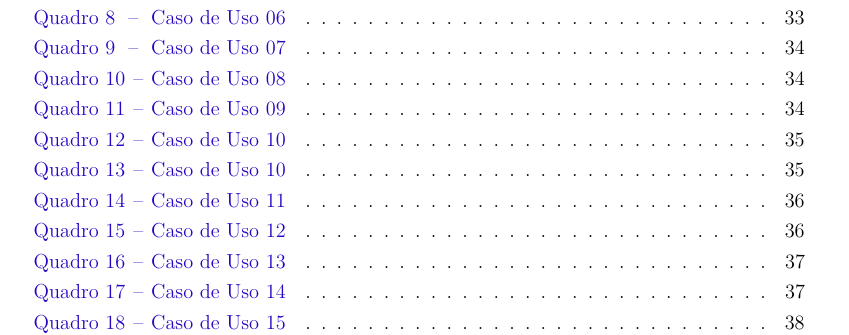
\includegraphics[width=0.9\textwidth]{erros/erros_lista_quadros.png}}
	\caption{\label{fig_erros_lista_quadros}Exemplo de Lista de quadros com erros comuns}
	\fonte{Trecho de um trabalho com o erro}
\end{figure}


\subsection{Erros em citações indiretas}
\label{erros-citacoes-indiretas}

As citações devem ficar em formato compatível com o texto onde ela estão localizadas. O tipo de citação deve ser escolhido corretamente para isso. O tipo de citação mais utilizado é a citação indireta, onde o o texto é escrito com suas próprias palavras e a referencia indicada.

Utilizar o texto de outra pessoa sem a citação da forma correta pode sr considerado plágio.

\todo[inline]{informações sobre plágio :  \url{https://www.ivanfm.com/plagio}}

O formato deve ser escolhido de acordo com o contexto utilizado :

\begin{itemize}
    \erradoerradocerto{utilizar o formato de citação errada, ver \autoref{referencias}}{de acordo com \cite{alcarde1996} ...}{de acordo com \citeauthor{alcarde1996} ...}{de acordo com \citeonline{alcarde1996}...}

% NBR 10520:2002 ver exemplos em 6.1.5
    \erradocerto{erro ao citar em final do paragrafo, o ponto final fica após a citação }{texto.\cite{alcione1988}} {texto \cite{alcione1988}. }


    \erradocerto{utilizar o formato de citação errada em fontes, ver \autoref{referencias}}{Fonte: \cite{alcarde1996}}{Fonte: \citeonline{alcarde1996}}

    \erradocerto{Erro na definição de publicações de organizações/empresas (ver definições de NBR6028 no arquivo .bib)}{sem utilizar \textbf{\emph{organization}} \cite{NBR6028:2003-errado}}{utilizando \textbf{\emph{organization}} \cite{NBR6028:2003}}
\end{itemize}


\subsection{Erros em citações diretas}
\label{erros-citacoes-diretas}

A \ac{abnt} define formatos específicos para citações diretas (aquelas onde é necessário colocar exatamente o que foi escrito pelo autor referenciado), citações curtas e citações longas (mais de 3 linhas). A citação curta é feita diretamente durante a escrita do texto, mas a citação longa deve ser feita de uma forma especifica. A \autoref{fig_citacao_longa_errada} demonstra a forma errada da citação e a \autoref{fig_citacao_longa_certa} mostra o formato correto para a citação longa.

\begin{figure}[hb]
    \centering
\fbox{\begin{minipage}{\textwidth}
Podemos observar que historicamente existem problemas que devem ser tratados: 
    ``\lipsum*[5]'' \cite{ETAL5}.
\end{minipage}}
    \caption{Citação direta longa - incorreta}
    \label{fig_citacao_longa_errada}
\end{figure}

\begin{figure}[hb]
    \centering
\fbox{\begin{minipage}{\textwidth}
Podemos observar que historicamente existem problemas que devem ser tratados: 
    \begin{citacao}
    \lipsum*[5] \cite{ETAL5}
    \end{citacao}
\end{minipage}}
    \caption{Citação direta longa - correta}
    \label{fig_citacao_longa_certa}
\end{figure}

%\newcommand{\video}[2]{\href{#1}{Vídeo: #2}}


\chapter{Erros comuns em projetos}
\label{erros-projetos}

Nesse capítulo estão apresentados os erros mais comuns que os professores observam nos sistemas desenvolvidos nas disciplinas de projetos. Alguns fazem parte de mais de uma categoria, mas foram listados cada um em uma categoria representada pela seção do documento.

São apresentados alguns problemas de projeto / modelagem e outros específicos do desenvolvimento.

Algumas referencias indicadas nesse capítulo são de publicações e vídeos disponíveis na internet que devem ser lidas / assistidos para correta compreensão do contexto.

O formato desse capítulo não segue exatamente o formato de documento indicado para os trabalhos acadêmicos.

\todo[inline]{Colocar aqui os erros mais comuns nos projetos de software das disciplinas}


\section{Erros de Processo}

Os processos da aplicação devem ser desenvolvidos de forma que o usuário possa utilizar a aplicação de maneira simples e intuitiva, existem casos onde o processo atual pode ser redefinido e criar ganhos, mas existem casos onde não é possível redefinir o processo real e o sistema deve atender a esse processo.

Muitas vezes o analista e o desenolvedor não se colocam no papel do usuário para verificar se o que estão desenvolvendo faz sentido para quem vai realmente utilizar a aplicação.

\begin{itemize}
    \item interface que não trata o processo de forma simples para o usuário (somente \gls{crud} e o usuário precisa saber qual sequencia deve utilizar);
    
    \item muitas bibliotecas e padrões abertos facilitam o desenvolvimento e simplificam a aplicação, normalmente não existe justificativa para \enquote{reinventar a roda}, ex: 
      \begin{itemize}
          \item utilização de \enquote{login social} OAuth;

          \item utilizações de bibliotecas para tratamentos básicos de segurança;
          
          \item utilizações de bibliotecas para validações.
      \end{itemize}
\end{itemize}

\section{Erros de Segurança}

\begin{itemize}
    \item implementação de um processo de recuperação de senha que depende de dados públicos : 
    Caso real que aconteceu com o sistema do ENEM - \citeonline{medicina_cachaca};
    \todo[inline]{migração para o biblatex para permitir a citação dos títulos}
    
    \item utilização de um meio de comunicação que não é seguro para envio de validação em etapa adicional : Caso real de invasão de Telegram a partir da vulnerabilidade da operadora de telefonia \cite{invasao_telegram};
    
    \item armazenamento de credenciais de acesso a banco de dados, servidor de e-mail diretamente dentro de arquivos da aplicação e que são colocados no repositório de controle de versão;
    
    \item armazenamento de senhas abertas no banco de dados (sem hash).
\end{itemize}

\section{Erros de modelo de dados}

\begin{itemize}
    \item Armazenamento de senhas abertas no banco de dados (sem hash);
    
    \item erro na definição dos modelos apresentados (físico, conceitual, lógico, DER, MER);
    
    \item erro na conversão entre modelos;
    
    \item dicionário de dados diferente da modelagem apresentada;
    
    \item tipagem de dados incorreta (Ex: um campo para data com tipo varchar);
    
    \item falta de índices adicionais em tabelas do banco de dados;

    \item falta de teste do modelo definido;
    
    \item exclusão física de dados que deveriam ser mantidos para histórico;
    
    \item falta de informações para auditoria de processos;
    
    
    
\end{itemize}

\section{Erros Interface com Usuário}

\begin{itemize}
    \item tradução automática de página via google tradutor, que acaba gerando falhas de contexto e traduções sem sentido;
    
    \item falta de responsividade em aplicações : web e móvel;
    
    \item não utilizar padrões já existentes para plataforma escolhida;
    
    \item interface complexa para o nível de conhecimento do público alvo da aplicação
    \newline
    \cite{computer_skills}.
    
\end{itemize}

\section{Erros de Validação}

\begin{itemize}
    \item Sistemas de cadastramento que não validam corretamente os dados : falta redigitação de campos importantes como senha;
    
    \item não validar corretamente os campos de acordo com definições existentes (ex e-mail deve seguir \citeonline[RFC 5322]{rfc5322});
    
    \item falta de validação de e-mail, se o e-mail não for válido o usuário não consegue recuperar a senha (não adianta validar somente o formato, tem que fazer envio com código de validação);
    
    \item Limites de senha sem considerar entropia da senha, ex uma senha grande é melhor que uma pequena com diversos tipos de caracteres \autoref{fig:password_strength};

    \item falta de tratamento no backend, fazendo validações e controle de acesso somente no frontend;
    
\end{itemize}

\begin{figure}
    \centering
	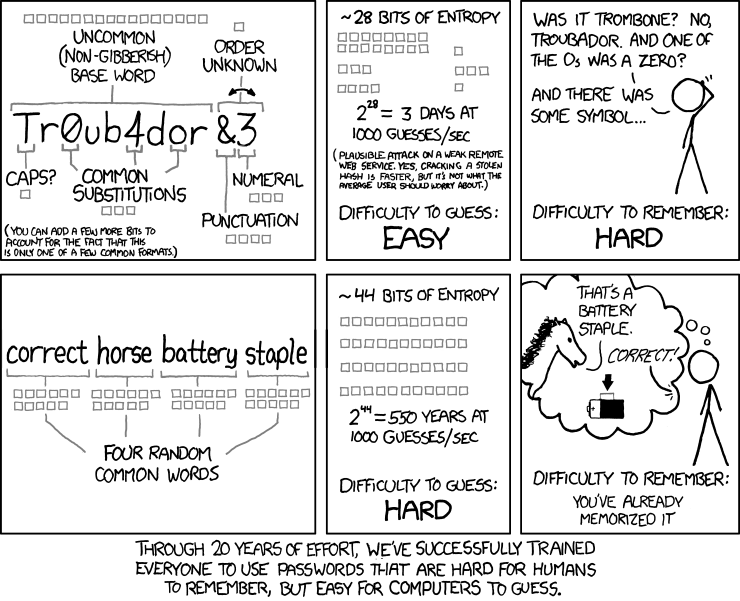
\includegraphics[width=0.95\textwidth]{erros/password_strength.png}
    \caption{Boas senhas não devem ser difíceis para o usuário}
    \fonte{\citeonline{fig_password_strength}}
    \label{fig:password_strength}
\end{figure}


\section{Erros do processo de teste e apresentação}

\begin{itemize}

    \item testar somente os casos de sucesso sem observar as condições de erro;
    
    \item volume de dados insuficiente para demonstrar o correto funcionamento da aplicação;
    
    \item falta de dados consistentes com o contexto da aplicação (escrever teste em um campo pode dificultar posteriormente a analise dos dados).
    
\end{itemize}

\section{Erros de modelagem / análise / projeto}

\begin{itemize}
    \item Casos de uso que não tratam corretamente as ações de usuários, ex recuperação de senha que tem dois passos (solicitação e redefinição da senha);
    
    \item definições de casos de uso ou estórias que não detalham o que deve ser feito 
    \newline
    % Instruções exatas como fazer um sanduiche com legendas
    \video{https://www.youtube.com/watch?v=pdhqwbUWf4U}{Como fazer um sanduíche};
    
    \item não analisar corretamente os dados disponíveis para o projeto \cite{boas_perguntas_dados} \cite{guerra-matematica} \cite{ellenberg2015poder} -  \autoref{fig:aviao_wald};

    
    \item desconsiderar o volume de dados e acessos da aplicação ao escolher a arquitetura.
\end{itemize}

\begin{figure}
    \centering
	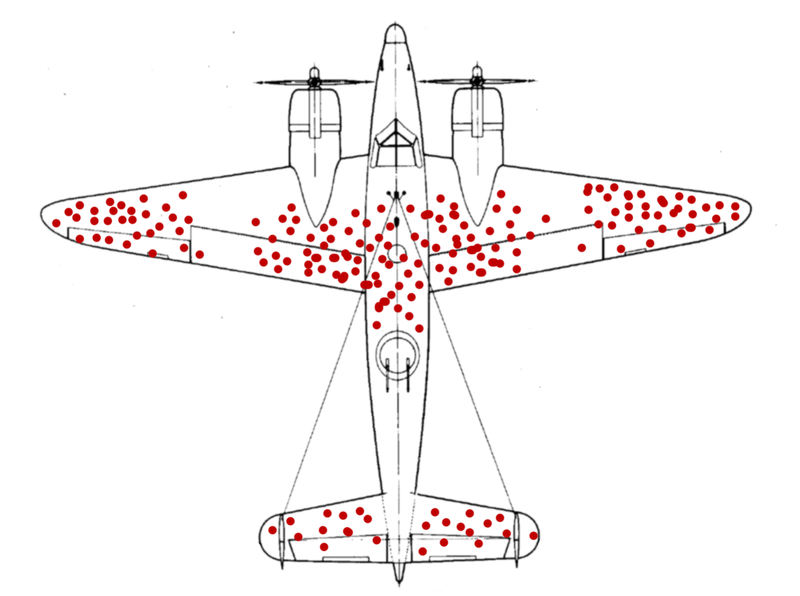
\includegraphics[width=0.8\textwidth]{erros/aviao_wald.png}
    \caption{Exemplo da análise de \citeonline{wald1980reprint} nos aviões sobreviventes da Segunda Guerra mundial}
    \fonte{\citeonline{fig_aviao_wald}}
    \label{fig:aviao_wald}
\end{figure}


\section{Erros de planejamento}

\begin{itemize}
    \item Escolher a metodologia X e não utilizar os itens básicos dessa metodologia no desenvolvimento do projeto;
    
    \item escolher XGH como metodologia de desenvolvimento \cite{xgh} \cite{xgh-axioms};
    
    \item quem planeja e escolhe a estratégia primeiro tem melhores resultados:
    \begin{itemize}
        \item 
        % Escolha a estratégia correta, corrida sobre tijolos
        \video{https://www.youtube.com/watch?v=4P-i9gCD09s&list=PL69253D27EBEF273E}{Escolha a estratégia correta};
        \item
        % Muito desgate sem planejamento, porquinho buscando cookies sobre geladeira
        \video{https://www.youtube.com/watch?v=LOyX-vgdQGQ&list=PL69253D27EBEF273E}{Muito desgate sem planejamento};
    
        \item % animação : Planejar é Preciso! LEGENDADO
        \video{https://www.youtube.com/watch?v=utLWFdkRm78&list=PL69253D27EBEF273E}{Planejar é Preciso}.    
    \end{itemize}
    
    \item falta de revisão em documentos, aplicação, vídeos;
    
    \item utilizar outras ferramentas e não as obrigatórias das disciplinas, um caso comum é a utilização da ferramenta Postman diretamente (criando a definição manualmente) em vez de utilizar o padrão OpenAPI (swagger) que é obrigatório e que pode ser importado no Postman \cite{postman-openapi};
    
    \item deixar para ultima hora, ex. processos como a criação de documentos no latexdiff, apesar de simples de executar, dependem de preparação de ambiente.
\end{itemize}



\section{Erros de comunicação}

\begin{itemize}
    \item Documentar da melhor maneira para garantir que todos entendam da mesma forma o que deve ser desenvolvido, cuidado com o que escreve:
    \begin{itemize}
        \item \autoref{fig:balanco};
        
        \item \autoref{fig:gabarito-prova};
        
        % Como fazer um sanduiche legendado....
        \item \video{https://www.youtube.com/watch?v=pdhqwbUWf4U&list=PL69253D27EBEF273E}{Como ensinar linguagem de programação para uma criança}.
    \end{itemize}

    \item não acompanhar o e-mail que recebe notificações do SUAP, moodle;
    
    \item não acompanhar o grupo da disciplina (normalmente no Telegram);
    
    \item falta de comunicação e negociação com os clientes.
\end{itemize}

\todo[inline]{Existem inúmeras versões dessa ilustração \autoref{fig:balanco}, aqui foi utilizada uma publicação como referencia para ilustrar a situação}

\begin{figure}
    \centering
	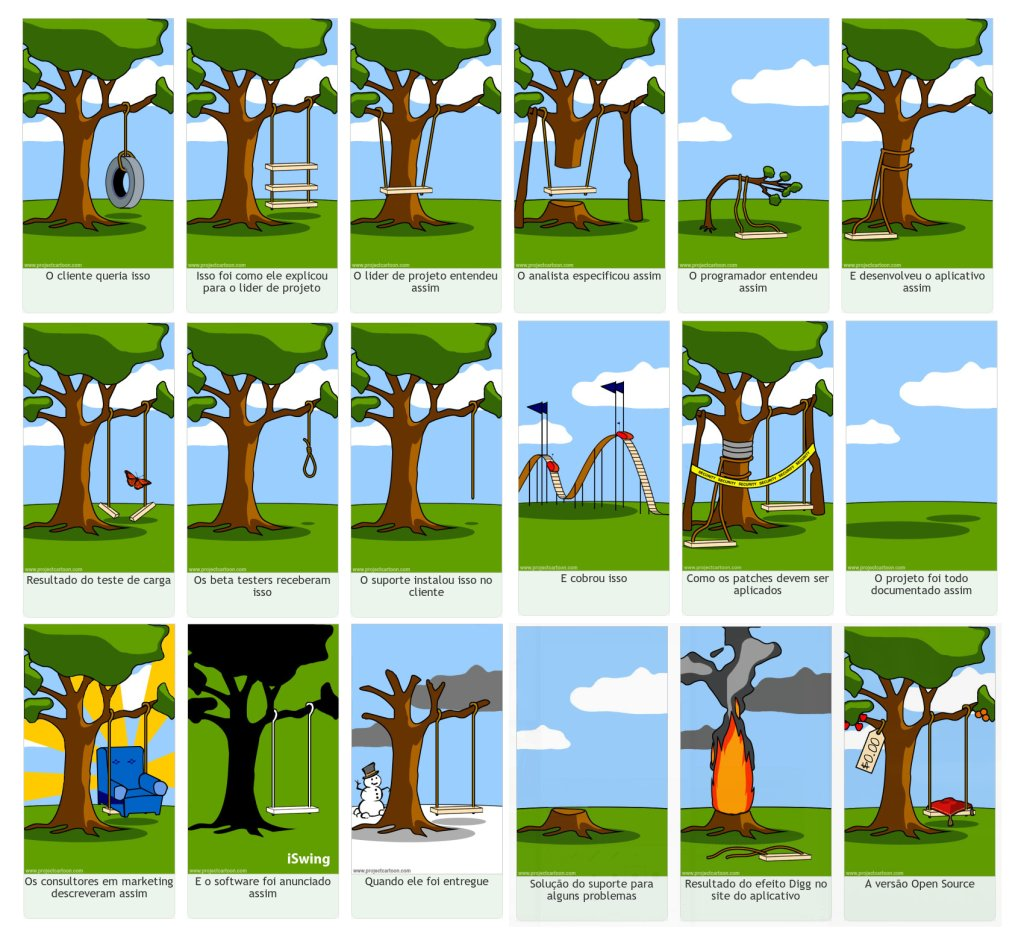
\includegraphics[width=0.95\textwidth]{erros/projeto_balanca_na_arvore.jpg}
    \caption{A importância da comunicação correta}
    \fonte{\citeonline{engenharia_software_balanca}}
    \label{fig:balanco}
\end{figure}


\begin{figure}
    \centering
	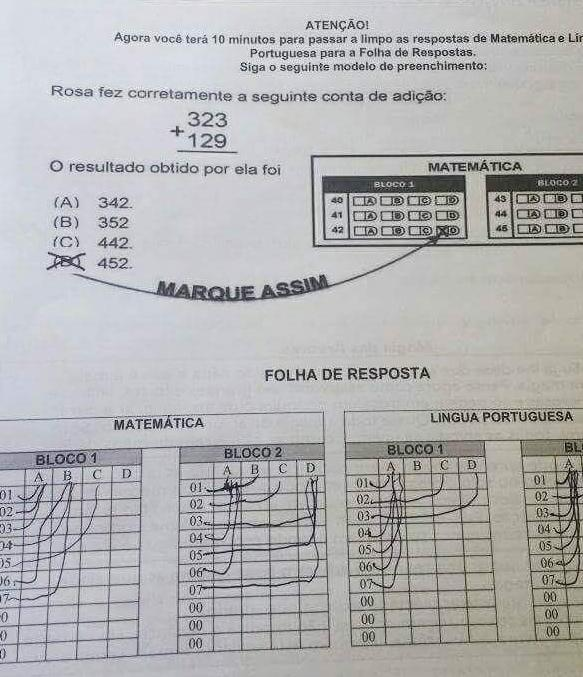
\includegraphics[width=0.95\textwidth]{erros/erro_de_comunicacao_gabarito_prova.jpg}
    \caption{A importância da comunicação correta 2}
% Fonte e titulo foram removidos propositalmente
    \label{fig:gabarito-prova}
\end{figure}



\section{Erros comportamentais}

Muitos insucessos acontecem devido a comportamentos dos participantes dos projetos, o histórico das disciplinas de projetos demonstraram diversos comportamentos individuais (alguns também acontecem com as equipes) que se evitados permitem melhores resultados:

\begin{itemize}
    \item falta de atenção na leitura dos documentos, regras das disciplinas, mensagens dos professores etc : \autoref{fig:vendo_bolo_cenoura} \cite{atencao_leitura_vendo_bolo_cenoura};
    
    \item medo de errar, para tomar as melhores decisões precisamos de experiencia, e experiencias muitas vezes vem de decisões erradas, mas é importante que essas experiencias aconteçam nos momentos corretos, no inicio e não no final dos projetos \cite{decisions_experience-1} \cite{decisions_experience-2} \autoref{fig:lidar_com_falhas};

    \item não entender o conceito de desenvolvimento de projeto em equipe e responsabilidades: 
    % Diversos videos sobre o trabalho em equipe 
    % Motivacional - Trabalho em equipe - Juntos fazemos mais e melhor!
    \video{https://www.youtube.com/watch?v=twg9SCt76UE&list=PL69253D27EBEF273E}{Trabalho em equipe - Juntos fazemos mais e melhor};
    
    \item não buscar as informações originais que normalmente se encontram em língua inglesa. Muitos documentos da área foram escritos em inglês e possuem traduções com erros técnicos, por isso é importante buscar os documentos originais e não utilizar traduções de terceiros;
    
    \item falta de foco: 
    % A importância de manter o foco!
    % Urso na fila de atendimento....
    \video{https://www.youtube.com/watch?v=6SRTQbBjrFs&list=PL69253D27EBEF273E}{A importância de manter o foco!};
    
    \item focar na tarefa e não no resultado:
    % fazendo trico / cachecol
    \video{https://www.youtube.com/watch?v=J0iv3TqJBV8&list=PL69253D27EBEF273E}{Foco na Tarefa x Foco no Resultado};
    
    \item falta de comprometimento: 
    \autoref{fig:scrum} e 
    \citeonline{meligeni_primeiro_treino};

    \item não acreditar no seu potencial: 
    % Desafio de Gigantes - carregando outro nas costas pelo campo todo...
    \video{https://www.youtube.com/watch?v=7UnyWuu8HK0&list=PL69253D27EBEF273E}{Trecho do filme Desafiando Gigantes - 2006}
    e
    % Rocky Balboa - Motivação Sensacional
    % Outras versões : 
    % https://www.youtube.com/watch?v=JeLYCrE5MrI
    % https://www.youtube.com/watch?v=Rhr6qO7Gmu0
    \video{https://www.youtube.com/watch?v=Qxsyy5H9JTk&list=PL69253D27EBEF273E}{Trecho do filme Rocky Balboa - 2006};
    
    \item medo de sair da zona de conforto:
    % Até a lagosta sente o desconforto do crescimento
    \video{https://www.youtube.com/watch?v=F8VBA89qWpc&list=PL69253D27EBEF273E}{Até a lagosta sente o desconforto do crescimento};
    
    \item falta de motivação, não encarar os desafios, pode ser falta de um \enquote{tubarão} \cite{tubarao_na_vida} \cite{put_a_shark_in_your_tank} \cite{employees_challenge};
    
    \item erro no gerenciamento do tempo e atividades:
    \begin{itemize}
        \item \enquote{macacos no ombro}:
    \waUrl{https://prazercompartilharblog.wordpress.com/2017/09/15/tire-os-macacos-do-meu-ombro/}
    e
    % TIRE O MACACO DO OMBRO
    \video{https://www.youtube.com/watch?v=7alQeDOtiRQ&list=PL69253D27EBEF273E}{TIRE O MACACO DO OMBRO});
    
        \item \video{https://www.youtube.com/watch?v=arj7oStGLkU}{Inside the mind of a master procrastinator} \cite{ted_tim_urban_procastinator}.
    \end{itemize}

    \item deixar para ultima hora o estudo das atividades (latexdiff, statsvn entre outras são ferramentas simples, mas dependem de preparação do ambiente para serem utilizadas);

    \item Não utilizar o conhecimento da equipe para resolver os problemas e fazer as escolhas - \autoref{fig:conhecimento_h2o};
    
    \item Não utilizar os recursos e ferramentas existentes da forma correta - \autoref{fig:uso_recursos_escada_1} \autoref{fig:uso_recursos_escada_2};

    \item Não aproveitar os aprendizados de outros alunos que já passaram pelas disciplinas de projetos :
    \begin{itemize}
        \item \waUrlTitle{https://glybif.blogspot.com.br/2016/12/como-ir-bem-em-pds.html}{Como ir bem em PDS? - GLYBIF - 2016};

        \item \waUrlTitle{https://glybif.blogspot.com/2020/04/4-anos-depois-de-fazer-pds.html}{4 anos depois de fazer PDS - GLYBIF - 2020};

        \item \waUrlTitle{https://projetothewalkingpet.blogspot.com/2018/12/dificuldades-e-licoes-aprendidas.html}{Dificuldades e lições aprendidas - The WalkingPet - 2018};

        \item \waUrlTitle{https://projetoa6pgpgrupo101010.blogspot.com/2018/12/o-que-nao-fazer-em-a6pgp-para-que-sofrer.html}{O que NÃO fazer em A6PGP: Para quê sofrer? - Blood 4 Pets - 2018};
        
        \item \waUrlTitle{https://projetoa6pgpgrupo101010.blogspot.com/2018/12/licoes-aprendidas-durante-o-semestre.html}{Lições aprendidas durante o semestre - Blood 4 Pets - 2018};

        \item \waUrlTitle{https://pgppain.blogspot.com/2019/03/19-coisas-que-voce-precisa-saber-sobre.html}{19 coisas que você precisa saber sobre a Prova de Conceito - PGPPain - 2019};

        \item \waUrlTitle{https://pgppain.blogspot.com/2019/03/nos-estamos-atrasados.html}{Nós estamos atrasados - PGPPain - 2019};

        \item \waUrlTitle{https://ginquestapp.wordpress.com/category/dicas-de-sobrevivencia/}{Dicas de Sobrevivência - GinQuest - 2019}.

    \end{itemize}
    
    \item falta de cuidado na comunicação dentro da equipe para garantir o objetivo.
    
\end{itemize}

\begin{figure}
    \centering
	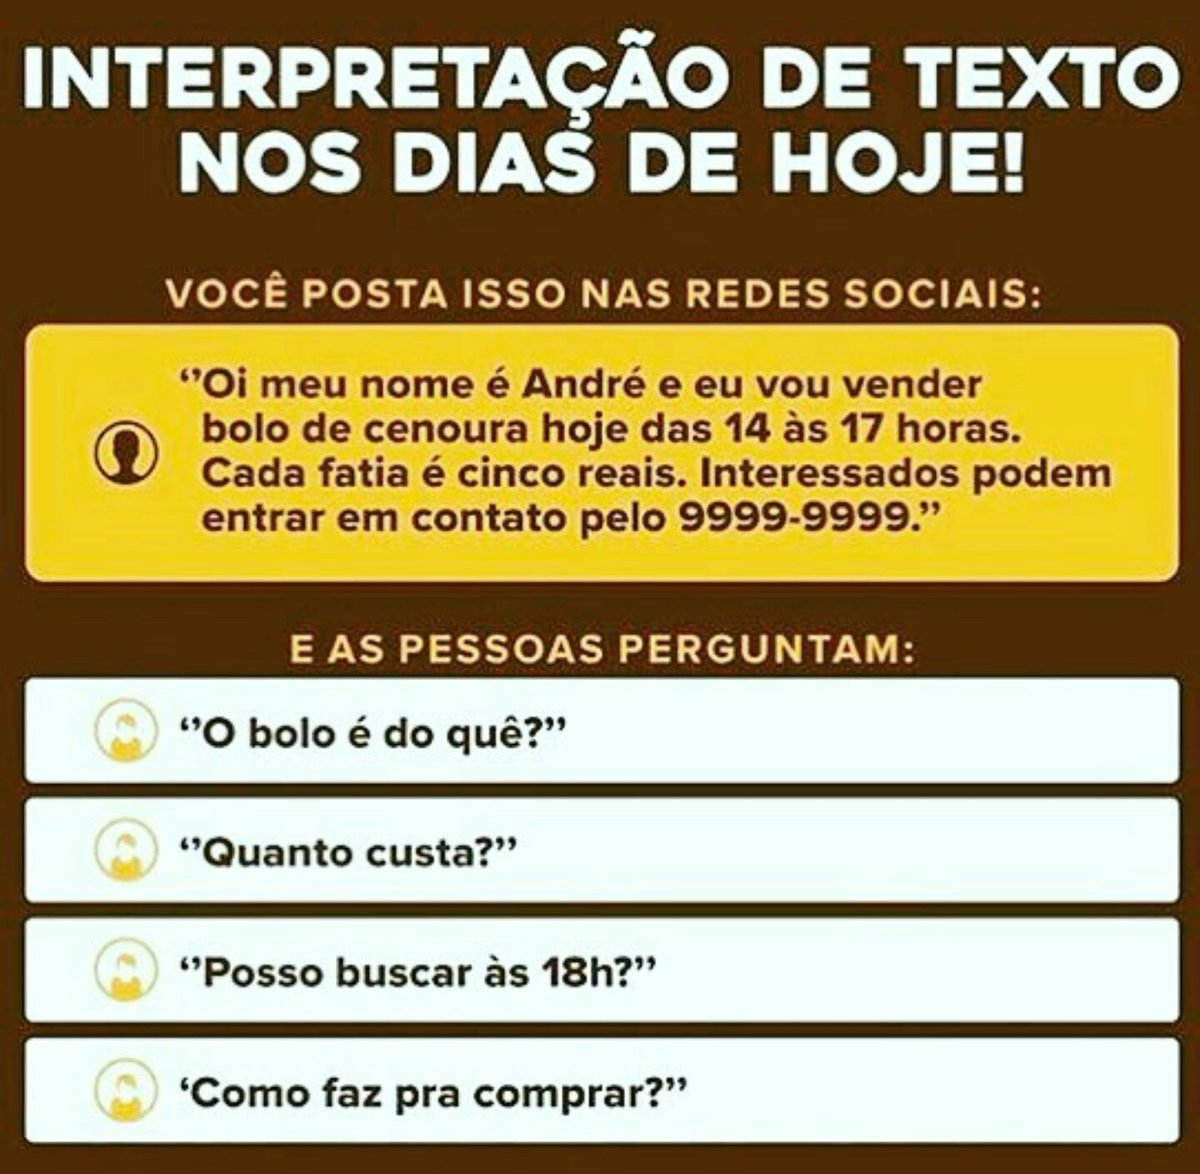
\includegraphics[width=0.95\textwidth]{erros/vendo_bolo_cenoura.jpg}
    \caption{Erro na interpretação das mensagens ou falta de atenção}
    \label{fig:vendo_bolo_cenoura}
\end{figure}



\begin{figure}
    \centering
	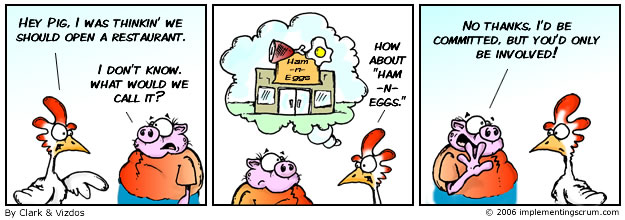
\includegraphics[width=0.95\textwidth]{erros/060911-scrumtoon.jpg}
    \caption{Comprometimento}
    \fonte{\citeonline{scrum_cartoon}}
    \label{fig:scrum}
\end{figure}

\begin{figure}
    \centering
	
\includegraphics[width=0.7\textwidth]{erros/conhecimento_h2o.jpg}
    \caption{Utilizar o conhecimento}
    \fonte{Hussein Awada, -}
    \label{fig:conhecimento_h2o}
\end{figure}

\begin{figure}
    \centering
	
\includegraphics[width=0.7\textwidth]{erros/uso_de_recursos_escada_1.jpg}
    \caption{Saiba utilizar corretamente seus recursos}
    \fonte{\citeonline{paulo_maciel_utilizar_recursos}}
    \label{fig:uso_recursos_escada_1}
\end{figure}

\begin{figure}
    \centering
	
\includegraphics[width=0.7\textwidth]{erros/uso_de_recursos_escada_2.jpg}
    \caption{Saiba utilizar corretamente seus recursos - Comparação}
    \fonte{\citeonline{paulo_maciel_utilizar_recursos_comparado}}
    \label{fig:uso_recursos_escada_2}
\end{figure}




\begin{figure}
    \centering
	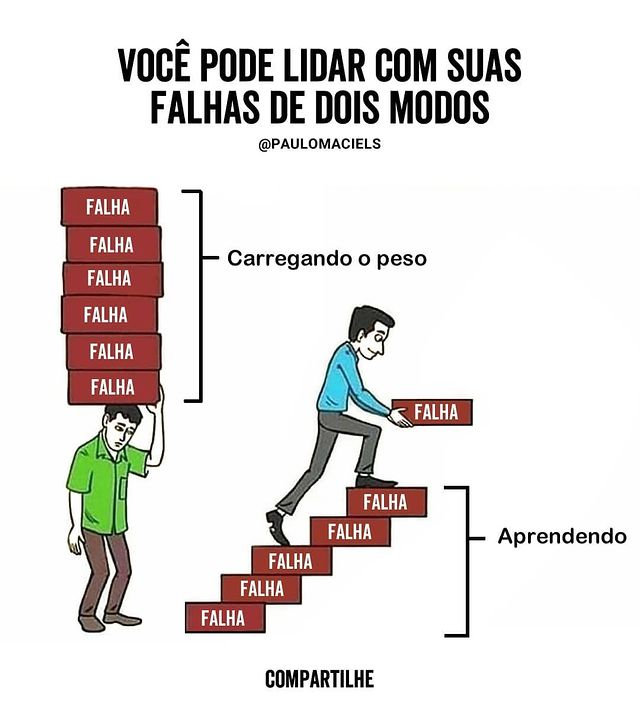
\includegraphics[width=0.7\textwidth]{erros/lidar_com_falhas.jpg}
    \caption{Aprenda a lidar com suas falhas}
    \fonte{\citeonline{paulo_maciel_lidar_com_falhas}}
    \label{fig:lidar_com_falhas}
\end{figure}


%\chapter{Revisão de Textos e apresentações}
\label{revisao-de-textos}

\todo[inline]{fazer as ligações com as seções de erros}

A revisão do documento e apresentação antes da entrega evita que os erros sejam apresentados no resultado final. Esse capítulo indica alguns procedimentos que evitam esse tipo de ocorrência.

\begin{itemize}
    \item Passar corretor ortográfico no documento;

    \item Faça a revisão em cima da versão final em \ac{pdf} com a formatação final;
    
    \item Utilize uma ferramenta de online de anotações no \ac{pdf} \url{https://dicas.ivanfm.com/aulas/textos/anotacoes-em-documentos.html} para facilitar o controle de anotações e histórico disponível para todos de forma online e centralizada;
    
    \item Solicite a diversas pessoas que participem da revisão, mesmo as pessoas que não entendem a parte técnica podem ajudar na revisão do texto;
    
    \item Coloque a data no nome do arquivo para facilitar a organização das versões compartilhadas;
    
    \item Para documentos gerados com \LaTeX, limpe todos os temporários / caches e compile do zero para garantir que todos os índices sejam atualizados;
    
    \item Verifique se a numeração das páginas é compatível com o formato de impressão (Frente/Verso ou somente Frente);
    
    \item Caso tenha páginas em A3 e impressão Frente/Verso cuidado para não alterar a posição das páginas na mudança;
    
    \item Verificar lista de siglas, siglas em outras línguas devem ter a tradução para português

    \item Verificar listas de figuras, quadros e tabelas - \autoref{revisao-listas};

    \item fazer buscas no documento para encontrar os erros mais comuns - \autoref{buscas-documento};
    
    \item Listas de itens devem ser separados ponto e virgula nos itens iniciais e ponto no último item;
    
    \item Listas de itens devem seguir uma ordem coerente (lógica ou alfabética) e não aleatória (por exemplo essa lista segue uma sequencia que considera uma ordem a ser seguida para executar a revisão);
    
    \item Não devem existir espaços em branco no meio dos capítulos, não forças quebras manualmente;
    
    \item verificar os tempos verbais (a leitura do documento acontece depois do desenvolvimento);
    
    \item Todos itens (capítulos, seções, subseções) devem possuir texto ( ideal que tenha pelo menos três parágrafos ) - ver \autoref{erros-comuns-sub1};

    \item Verificar palavras de outras línguas - ver \autoref{revisao-palavras-estrangeiras};
    
    \item Padronização de nomenclatura : o é \textbf{XYZ} ou \textbf{Xyz} utilizar um único formato em todos locais.
    
\end{itemize}

\section{Verificação das listas de elementos do documento}
\label{revisao-listas}

As listas de ilustrações (figuras, quadros, tabelas etc) e o sumário devem ser verificadas com cuidado :

\begin{itemize}
    \item não devem conter elementos com mesmo titulo, cada elemento deve ter um titulo único;
    
    \item caso existam vários elementos parecidos verifique se o formato de nomes segue um mesmo padrão.
    \todo[inline]{vale criar um exemplo na seção de erros}
    
\end{itemize}

\section{Buscas que podem encontrar problemas no documento}
\label{buscas-documento}

\begin{itemize}
    \item \textbf{??} para encontrar referências quebradas, já que o \LaTeX \space indica com \textbf{??} quando não encontra uma referencia;
    
    \item Buscar por \textbf{Figura}, \textbf{Quadro}, \textbf{Tabela} etc
    
        \begin{itemize}
            \item verificar se os artigos ( feminino / masculino ,  a / o  ) estão corretos;
           
            \item Verificar se tabelas e quadros foram definidos corretamente ;
           
            \item Colunas com valores numéricos em tabelas / quadros devem ser alinhadas à direita;
           
            \item Verificar se toda ilustração foi citada no texto;
           
            \item Verificar se gráfico colorido vai ficar legível na impressão preto e branco;
            
            \item Verificar se as citações e referencias estão como links (no caso do \LaTeX \space utilizando esse modelo ficam em cor azul);
          
            \item Verifique se as referencias do texto para as ilustrações estão na sequencia correta (a \textbf{figura n} deve ser referenciada antes da \textbf{figura n+x}).  
        \end{itemize}
        
    \item Buscar por cada elemento da lista de siglas / abreviações - ver \autoref{buscas-siglas};
    
    \item Buscar por cada elemento do glossário - ver \autoref{buscas-glossario};
            
    \item Buscar por \textbf{"} (aspas), verificar se não está grudada no texto anterior / seguinte;
    
    \item Buscar por \textbf{(} para verificar citações - ver \autoref{erros-citacoes-indiretas}
        \begin{itemize}
            \item Verificar se o formato da citação é compatível com o texto / local onde se encontram;
            
            \item Verificar se citações não ficaram grudadas no texto.
        \end{itemize}
            
    \item Buscar por \textbf{[S.l.]}, vai encontrar referencias incompletas de livros.
\end{itemize}

\section{Revisão de siglas}
\label{buscas-siglas}

As siglas (ex \ac{ifsp}) devem seguir um padrão dentro do documento, buscar por cada elemento na lista de siglas permite determinar se foram definidas corretamente :

\begin{itemize}
    \item Primeira ocorrência deve ter nome por extenso.
    
    \item No documento gerado com \LaTeX \space todas utilizações devem ser links.
\end{itemize}

Mas se durante a leitura do documento encontrar alguma sigla que não esteja indicada com o link essa sigla não foi definida corretamente dentro do documento \LaTeX  \space como uma sigla.

\section{Revisão de glossário}
\label{buscas-glossario}

Como o \LaTeX \space faz a referencia de glossário como um link é importante buscar no documento pelas palavras do glossário e verificar se estão com o link. Também é importante solicitar que os revisores que não fazem parte da escrita do documento anotem os termos que tem dúvidas já que isso é um bom indicador de palavras que devem ser incluídas no glossário.


\section{Revisão de Palavras de outras Línguas}
\label{revisao-palavras-estrangeiras}

De acordo com a \ac{abnt} as palavras estrangeiras devem ser utilizadas com itálico (exceto nomes próprios), mas também deve ser tomado o cuidado já que muitas vezes precisamos incluir um artigo juntamente com a palavra, portanto é necessário verificar  se está utilizando artigo de forma correta :

\begin{itemize}
    \item \textbf{o \emph{sprint}} ou \textbf{a \emph{sprint}} são validos mas deve ser utilizado de forma uniforme em todo o texto e de acordo com a definição utilizada 
    \begin{itemize}
        \item se \emph{sprint} for definido como um período de tempo, ciclo de desenvolvimento deve utilizar o artigo \textbf{o};
        
        \item se a definição é como uma etapa ou fase de desenvolvimento deve utilizar o artigo \textbf{a}.
    \end{itemize}
    
\end{itemize}


\section{Revisão de Apresentações}
\label{revisao-apresentacoes}

Em apresentações alguns detalhes adicionais devem ser considerados como contraste entre os elementos utilizados e se cores forem utilizadas para demonstrar alguma informação se todos podem ver essa informação (considerando que algumas pessoas não conseguem visualizar todas as cores é sempre bom utilizar ícones na representação. Se a apresentação for feita com o uso de um projetor é importante testar antecipadamente para garantir que o projetor consiga apresentar corretamente as cores e resolução utilizadas.







%% ---
% Conclusão (outro exemplo de capítulo sem numeração e presente no sumário)
% Dependendo do trabalho desenvolvido ele pode ter uma Conclusão ou Considerações finais
% Para trabalhos de disciplina utilizar Considerações Finais
% ---
\chapter*{Considerações Finais}
\addcontentsline{toc}{chapter}{Considerações Finais}
% Para definir com número utilizar sem o asterisco
%\chapter{Considerações finais}


% ---
Além desse documento ser um modelo de como pode ser criado um documento em \LaTeX \space ele também apresenta diversas informações úteis para as disciplinas de projetos de informática do \ac{ifsp} e alguns elementos uteis para as monografias do curso de Pós Graduação em Gestão de TI do \ac{ifsp}.



\explicacao{Exemplo de seções para monografia da pós graduação...}
\section{Resposta à Questão de Pesquisa}
\lipsum[3-5]

\section{Objetivos Propostos}
\lipsum[3-5]

\section{Contribuições Acadêmicas e Gerenciais}
\lipsum[3-5]

\section{Limitações da Pesquisa e Contribuições para Estudo}
\lipsum[3-5]


% ----------------------------------------------------------
% Finaliza a parte no bookmark do PDF
% para que se inicie o bookmark na raiz
% e adiciona espaço de parte no Sumário
% ----------------------------------------------------------
% \phantompart

% ----------------------------------------------------------
% ELEMENTOS PÓS-TEXTUAIS
% ----------------------------------------------------------
%\postextual
% ----------------------------------------------------------

% ----------------------------------------------------------
% Referências bibliográficas
% ----------------------------------------------------------
% quando não esta utilizando biblatex tem que carregar as referencias aqui
\IfPackageLoaded{biblatex}{}{%
\bibliography{referencias,exemplos/abntex2-doc-abnt-6023}
}

% ----------------------------------------------------------
% Glossário
% ----------------------------------------------------------
%

 \ifdef{\printnoidxglossary}{
     \addcontentsline{toc}{chapter}{GLOSSÁRIO}
     \printnoidxglossary[style=glossario]
}{}

%% ----------------------------------------------------------
% Apêndices
% Documentos gerados pelo próprio autor
% ----------------------------------------------------------

% ---
% Inicia os apêndices
% ---
\begin{apendicesenv}

% Imprime uma página indicando o início dos apêndices
\partapendices
% ----------------------------------------------------------
\chapter{Proposta Inicial}
% ----------------------------------------------------------

\includepdf[pages=-]{EntregaFinal/PropostaInicial.pdf}

% ----------------------------------------------------------
\chapter{Sprints}
\label{sprints-atividades}
% ----------------------------------------------------------

Esta seção apresenta as atividades planejadas em cada \gls{sprint}.


\section{Sprint 1 - 10/05/2021 a 25/05/2021}

O \autoref{quadro-sprint1} mostra a divisão de tarefas da equipe ao longo da sprint.

\begin{quadro}[htb]
\centering
\ABNTEXfontereduzida
\caption{Sprint 1 - 10/05/2021 a 25/05/2021}
\label{quadro-sprint1}
\begin{tabular}{|l|c|}
\hline
{\thead{Atividade}} & \thead{Responsável}  \\ \hline
    Concepção do Projeto & André     \\ \hline 
    Concepção do Projeto & Bianca     \\ \hline
    Concepção do Projeto & Luiz      \\ \hline
    Concepção do Projeto & Natan   \\ \hline
    Concepção do Projeto & Patrícia    \\ \hline
    Pesquisa sobre outras aplicações  & André     \\ \hline  
    \multicolumn{2}{|c|}{Proposta Inicial} \\ \hline
    Justificativa                     & Natan    \\ \hline
    Objetivo                          & Luiz     \\ \hline
    Escopo                            & Patrícia \\ \hline
    Integrações                       & André     \\ \hline   
    Tecnologia e Infraestrutura       & André     \\   \hline
    Tecnologia e Infraestrutura       & Patrícia  \\ \hline
    Parcerias e Viabilidade Comercial & Patrícia \\ \hline 
    Revisão da Documentação           & Bianca   \\ \hline  
    Apresentação                      & Bianca  \\ \hline 
    \multicolumn{2}{|c|}{Blog} \\ \hline
    Postagem - Semana 01      & Bianca  \\ \hline
    Postagem - Semana 02      & Bianca     \\ \hline
\end{tabular}
\fonte{Os autores}
\end{quadro}
\FloatBarrier

\section{Sprint 2 - 25/05/2021 a 08/06/2021}
O \autoref{quadro-sprint2} demonstra as atividades concluídas na Sprint 2.
\begin{quadro}[htb]
\centering
\ABNTEXfontereduzida
\caption{Sprint 2 - 25/05/2021 a 08/06/2021}
\label{quadro-sprint2}
\begin{tabular}{|l|c|}
\hline
{\thead{Atividade}} & \thead{Responsável}  \\ \hline  
    \multicolumn{2}{|c|}{Proposta Inicial} \\ \hline
    Ajustes - Justificativa           & Patrícia     \\ \hline
    Ajustes - Objetivo                & Patrícia     \\ \hline
    Detalhamento do Escopo            & Patrícia \\ \hline
    Ajustes - Escopo                  & Patrícia    \\ \hline   
    Ajustes - Análise Comparativa       & Natan      \\   \hline
    Ajustes - Análise Comparativa       & Bianca \\ \hline
    Evoluções Previstas  & Patrícia \\ \hline 
    Ajustes - Integrações          & Natan \\ \hline  
    Ajustes - Tecnologias            & Natan   \\ \hline 
    Ajustes - Tecnologias                   & Luiz  \\ \hline 
    Monetização    & Bianca  \\ \hline 
    Monetização    & Natan  \\ \hline 
    Suporte nos Ajustes  & André   \\ \hline 
    Formatação da Documentação & Patrícia  \\ \hline 
    Formatação da Documentação & Luiz   \\ \hline 
    Revisão da Documentação & Bianca   \\ \hline 
    Ajustes - Apresentação & Bianca  \\ \hline 
    
    \multicolumn{2}{|c|}{Desenho da Aplicação} \\ \hline
    Introdução  & Natan  \\ \hline 
    Revisão Bibliográfica  & Natan  \\ \hline 
    Arquitetura da Solução  & Patrícia   \\ \hline 
    Escopo  & Patrícia  \\ \hline 
    Escopo  & Bianca   \\ \hline 
    Viabilidade Financeira  & Natan  \\ \hline 
    Escalabilidade  & Patrícia  \\ \hline 
    Segurança  & Luiz  \\ \hline 
    Tecnologias  & Luiz \\ \hline 
    Manutenibilidade da aplicação  & Patrícia   \\ \hline 
    Metodologias  & Bianca  \\ \hline 
    Revisão da Documentação  & Luiz \\ \hline 
    
    \multicolumn{2}{|c|}{Desenvolvimento do Back-End} \\ \hline
    Criar repositório no github & André  \\ \hline 
    Preparação do ambiente & André  \\ \hline 
    Configuração do banco de dados em produção & André  \\ \hline 
    Autenticação pelo firebase & André  \\ \hline 
    Fluxo de primeiro acesso & André  \\ \hline 
    Teste de primeiro acesso (integração) & André  \\ \hline 
    
    \multicolumn{2}{|c|}{Desenvolvimento do Front-End} \\ \hline
    Criar repositório no github & André  \\ \hline 
    Criar tela de login & André  \\ \hline 
    Criar tela de novo acesso & André \\ \hline 
    
    \multicolumn{2}{|c|}{Blog} \\ \hline
    Postagem - Semana 03      & Bianca      \\ \hline
    Postagem - Semana 04      & Bianca      \\ \hline
    
    \multicolumn{2}{|c|}{Vídeo} \\ \hline
    Gravar o vídeo da proposta inicial & Natan  \\ \hline 
\end{tabular}
\fonte{Os autores}
\end{quadro}
\FloatBarrier

\section{Sprint 3 - 08/06/2021 a 22/06/2021}
O \autoref{quadro-sprint3} representa as atividades realizadas ao longo da sprint.
\begin{quadro}[htb]
\centering
\ABNTEXfontereduzida
\caption{Sprint 3 - 08/06/2021 a 22/06/2021}
\label{quadro-sprint3}
\begin{tabular}{|l|c|}
\hline
{\thead{Atividade}} & \thead{Responsável}  \\ \hline
    \multicolumn{2}{|c|}{Desenho da Aplicação} \\ \hline
    Ajustes - Lista de Siglas           & Natan     \\ \hline
    Ajustes - Introdução                          & Natan \\ \hline
    Ajustes - Arquitetura de Solução              & Patrícia \\ \hline
    Ajustes - Escopo                       & Bianca     \\ \hline   
    Ajustes - Viabilidade Financeira       & Natan   \\   \hline
    Ajustes - Metodologias       & Bianca \\ \hline
    Ajustes - Product Backlog & Patrícia  \\ \hline 
    Revisão da Documentação           & Natan \\ \hline  
    Configuração do LaTeX diff     & Natan   \\ \hline 
    Apresentação 		 & Bianca  \\ \hline
    
     \multicolumn{2}{|c|}{Histórias de Usuário} \\ \hline
     Administrador & André  \\ \hline
     Gestor & Luiz   \\ \hline
     Professor & Bianca \\ \hline
     Aluno & Patrícia  \\ \hline
     Criar mais histórias de usuário & Patrícia  \\ \hline
    
    \multicolumn{2}{|c|}{Desenvolvimento do Back-End} \\ \hline
    Autenticação e Autorização & André \\ \hline 
    Cadastro e Visualização do Administrador & André  \\ \hline 
    Envio de e-mail do primeiro acesso & André \\ \hline 
    
    \multicolumn{2}{|c|}{Desenvolvimento do Front-End} \\ \hline
    Elaboração de Protótipos de baixa fidelidade & André \\ \hline 
    Elaboração de Protótipos de baixa fidelidade & Luiz  \\ \hline 
    
    \multicolumn{2}{|c|}{Blog} \\ \hline
    Postagem - Semana 05      & Bianca    \\ \hline
    Postagem - Semana 06      & Bianca   \\ \hline
    
    \multicolumn{2}{|c|}{Vídeo} \\ \hline
    Gource & Natan \\ \hline
    
\end{tabular}
\fonte{Os autores}
\end{quadro}
\FloatBarrier

\section{Sprint 4 - 22/06/2021 a 06/07/2021}
 A Sprint 4 foi principalmente dedicada às entregas da POC e ajustes no desenho da aplicação. O \autoref{quadro-sprint4} representa as atividades realizadas ao longo da sprint.
 
\begin{quadro}[htb]
\centering
\ABNTEXfontereduzida
\caption{Sprint 4 - 22/06/2021 a 06/07/2021}
\label{quadro-sprint4}
\begin{tabular}{|l|c|}
\hline
{\thead{Atividade}} & \thead{Responsável}  \\ \hline
    \multicolumn{2}{|c|}{Desenho da Aplicação} \\ \hline
    Tag SVN           & Natan   \\ \hline
    \multicolumn{2}{|c|}{Prova de Conceito} \\ \hline
    Ajustes no código                     & André     \\ \hline
    Subir no SVN                & Bianca  \\ \hline
    Apresentação                & André \\ \hline
    Relatório                       & André     \\ \hline   
    Formatação LaTeX       & Natan      \\   \hline
    Vídeo       & Natan  \\ \hline
    Desenhar arquitetura & Patrícia   \\ \hline 
    Tags SVN           & Natan   \\ \hline  
    
    \multicolumn{2}{|c|}{Desenvolvimento do Back-End} \\ \hline
    Criar listagem e paginação de administradores cadastrados & André    \\ \hline   
    Arrumar fluxo de login e primeiro acesso & André    \\ \hline 
    Criar cadastro de escolas & André    \\ \hline   
    Aumentar cobertura de testes & André    \\ \hline  
    Exclusão de administradores & Patrícia   \\ \hline 
    
    \multicolumn{2}{|c|}{Desenvolvimento do Front-End} \\ \hline
    Criar tela de cadastro de escolas & André   \\ \hline 
    Elaboração de Protótipos de alta fidelidade & Patrícia   \\ \hline 
    Elaboração de Protótipos de alta fidelidade & Luiz  \\ \hline 
    
    \multicolumn{2}{|c|}{Blog} \\ \hline
    Ajustes no conteúdo  & Bianca      \\ \hline
    Postagem - Semana 07      & Bianca     \\ \hline
    Postagem - Semana 08      & Bianca      \\ \hline
    
    \multicolumn{2}{|c|}{Vídeo} \\ \hline
    Gource (POC) & Natan   \\ \hline 
    Gravação do vídeo (Desenho da Aplicação) & Bianca     \\ \hline
    Gravação do vídeo (Desenho da Aplicação) & Luiz   \\ \hline
    Gravação do vídeo (Desenho da Aplicação) & Natan   \\ \hline
    Gravação do vídeo (Desenho da Aplicação) & Patrícia    \\ \hline
    
    \multicolumn{2}{|c|}{LaTeX} \\ \hline
    Adequação dos arquivos em LaTeX & Natan   \\ \hline 
    Subir no SVN & Natan   \\ \hline
    
\end{tabular}
\fonte{Os autores}
\end{quadro}
\FloatBarrier

\section{Sprint 5 - 06/07/2021 a 20/07/2021}
Com as datas de entrega da documentação final e da apresentação próximas, dedicou-se um maior tempo ao desenvolvimento do projeto. O \autoref{quadro-sprint5} representa as atividades realizadas ao longo da sprint.
\begin{quadro}[htb]
\centering
\ABNTEXfontereduzida
\caption{Sprint 5 - 06/07/2021 a 20/07/2021}
\label{quadro-sprint5}
\begin{tabular}{|l|c|}
\hline
{\thead{Atividade}} & \thead{Responsável} \\ \hline
    \multicolumn{2}{|c|}{Documentação Final} \\ \hline
    Ajustes na estrutura do documento & Bianca \\ \hline
    Ajustes - Revisão de Literatura & Bianca   \\ \hline 
    Atividades das sprints       & Bianca  \\ \hline
    Postagens do blog  & Bianca  \\ \hline
    Métricas do projeto  & Bianca    \\ \hline   
    Proposta Inicial  & Bianca    \\ \hline  
    QR Codes       & Luiz    \\   \hline
    QR Codes       & Natan      \\   \hline
    Escolhas e Descartes       & Luiz  \\ \hline
    Escolhas e Descartes & Bianca   \\ \hline 
    Ajustes - Escopo & Bianca   \\ \hline 
    Modelagem de Dados & Natan   \\ \hline 
    Testes Front-end & Patricia  \\ \hline 
    Testes Back-end & Bianca   \\ \hline 
    Entregáveis & Bianca  \\ \hline 
    Ajustes - Segurança & Bianca  \\ \hline 
    Considerações Finais   & Bianca    \\ \hline  
    
    \multicolumn{2}{|c|}{Desenvolvimento do Back-End} \\ \hline
    Cadastro de conquista & André    \\ \hline  
    Entrega de conquista & André    \\ \hline 
    CRUD de gestores & André    \\ \hline  
    CRUD de alunos & André    \\ \hline  
    CRUD de professores & André   \\ \hline 
    Endpoint cadastro de turma & André    \\ \hline
    Endpoint cadastro de atividades & André     \\ \hline  
    Busca dinâmica de escolas & Natan   \\ \hline 
    Busca dinâmica de administradores & Natan   \\ \hline 
    Busca dinâmica de gestores & Natan   \\ \hline 
    Busca dinâmica de professores & Natan   \\ \hline
    Criação dos loaders & Gustavo   \\ \hline 
    Traduções dos placeholders & Gustavo \\ \hline 
    Tratamento de erros nos formulários & Gustavo  \\ \hline 
    Aumentar cobertura de testes & André      \\ \hline 
    
    \multicolumn{2}{|c|}{Desenvolvimento do Front-End} \\ \hline
    Configuração do Cypress & André    \\ \hline 
    Tela do cadastro de turmas & André  \\ \hline 
    Tela do cadastro de atividades & André   \\ \hline
    Listagem de turmas & André \\ \hline 
    Visão do professor & André  \\ \hline 
    Tela de criação de professor & Gustavo   \\ \hline 
    Testes de Escolas & Patricia \\ \hline 
    Testes de Administradores & Patricia  \\ \hline 
    Testes de Gestores & Patricia  \\ \hline 
    Testes de Professores & Patricia  \\ \hline 
    Configurar relatórios de testes & Patricia  \\ \hline 
    Estilização de telas & Patricia \\ \hline 
    
    \multicolumn{2}{|c|}{Blog} \\ \hline
    Postagem - Semana 09      & Bianca      \\ \hline
    Postagem - Semana 10      & Bianca   \\ \hline
    
    \multicolumn{2}{|c|}{Vídeo} \\ \hline
    Gource (POC) & Natan  \\ \hline 
    
    
\end{tabular}
\fonte{Os autores}
\end{quadro}
\FloatBarrier

\section{Sprint 6 - 20/07/2021 a 03/08/2021}
No período da Sprint 6, iniciou-se as provas das outras disciplinas, por conta disso não foi possível dedicar-se tanto ao projeto. O \autoref{quadro-sprint6} representa as atividades realizadas ao longo da sprint.

\begin{quadro}[htb]
\centering
\ABNTEXfontereduzida
\caption{Sprint 6 - 20/07/2021 a 03/08/2021}
\label{quadro-sprint6}
\begin{tabular}{|l|c|}
\hline
{\thead{Atividade}} & \thead{Responsável}  \\ \hline
    \multicolumn{2}{|c|}{Documentação Final} \\ \hline
    Ajustes gerais no documento                & Bianca  \\ \hline
    Ajustes gerais no documento                & Luiz \\ \hline
    Apresentação final               & Bianca  \\ \hline
    
    \multicolumn{2}{|c|}{Desenvolvimento do Back-End} \\ \hline
    Listagem de Atividades & André    \\ \hline  
    Envio de anexos & André    \\ \hline 
    Entrega de Atividades & André    \\ \hline   
    Encerramento de turmas & André    \\ \hline  
    
    \multicolumn{2}{|c|}{Desenvolvimento do Front-End} \\ \hline
    Validação dos formulários de atividades & Gustavo   \\ \hline 
    Ajustes nas validações dos campos & Gustavo   \\ \hline 
    Aprofundamento do entendimento do Cypress & Patrícia   \\ \hline 
    Aumento da cobertura de testes & Patrícia   \\ \hline 
    
    \multicolumn{2}{|c|}{Blog} \\ \hline
    Postagem - Semana 11      & Bianca     \\ \hline
    Postagem - Semana 12      & Bianca      \\ \hline
    
    \multicolumn{2}{|c|}{Vídeo} \\ \hline
    Gource (MVP) & Natan   \\ \hline 
    
    \multicolumn{2}{|c|}{LaTeX} \\ \hline
    Subir no SVN & Luiz   \\ \hline
    Suporte na subida para o SVN & Natan   \\ \hline
    
\end{tabular}
\fonte{Os autores}
\end{quadro}
\FloatBarrier

\section{Sprint 7 - 03/08/2021 a 17/08/2021}
Como um dos pontos levantados pelos professores da banca foi que a equipe não estava seguindo a metodologia ágil da forma correta, foi necessária uma reestruturação na metodologia adotada. Para isso, passou-se a fazer o Sprint Backlog no kanban do GitHub. Dessa forma, é possível unificar as tarefas feitas com os respectivos códigos, além de melhorar a criação de métricas para o projeto. A \autoref{sprint7} demonstra o kanban criado para o Sprint Backlog.

\begin{figure}[htb]
    \centering
	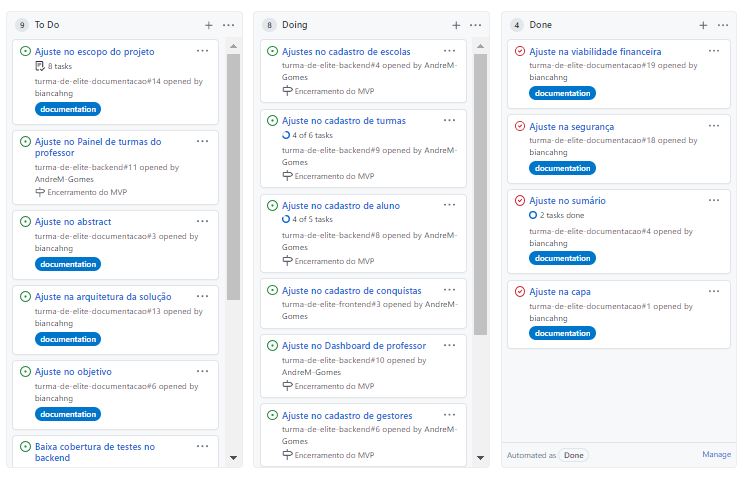
\includegraphics[width=16cm]{imagens/sprint7.png}
	\caption{\label{sprint7} Sprint Backlog da sprint 7}
	\fonte{Os autores}
\end{figure}
\FloatBarrier

% ----------------------------------------------------------
\chapter{Publicações do Blog}
% ----------------------------------------------------------

Ao longo do desenvolvimento do projeto, foram feitas postagens semanais no blog a respeito das atividades exercidas por cada integrante, sobre as reuniões realizadas e decisões tomadas pela equipe.

\section{Resumo de Atividades - Semana 1}

Esse blog tem como objetivo mostrar um acompanhamento semanal do projeto que estamos desenvolvendo para a disciplina de Projeto Integrado I (PI1A5).

Na primeira semana, definimos os integrantes da equipe:

\begin{itemize}
\item André Monteiro Gomes;
\item Bianca Kaori Hng;
\item Luiz Henrique de Almeida e Albuquerque;
\item Natan da Fonseca Lisboa;
\item Patricia Santos Paschoal.
\end{itemize}

E como ideia principal foi decidido que seria algo voltado para a educação, devido à proximidade de alguns dos integrantes com a área e também devido ao fato de já houver alguns esboços de ideias relacionados a isso pelos próprios integrantes. 

A metodologia de gestão adotada foi o Scrum e a gerente do projeto escolhida fui eu, Bianca.

Então, a Patrícia começou a elicitar possíveis requisitos para a aplicação e o André, possíveis tecnologias a serem usadas.

O nome escolhido para a equipe foi "DevAneios", sugerido pelo Natan e, para o nome do projeto, foi escolhido "Turma de Elite", sugerido pelo Luiz. E eu, Bianca, criei o canal do YouTube e o Blog para o projeto.

Fizemos uma reunião com todos os integrantes e, assim, ficou decidido que o projeto aplicaria conceitos de gamificação para a execução de atividades, com o objetivo de incentivar os alunos a desenvolverem as tarefas.


\section{Resumo de Atividades - Semana 2}
Apresentamos a ideia do projeto para o professor e esta foi aceita por ele com a orientação de aprofundá-la para a apresentação da próxima semana. 

Então, a segunda semana foi dedicada ao amadurecimento da ideia e a elaboração do documento e a apresentação da proposta inicial para a turma. 

Nos reunimos duas vezes ao longo da semana: a primeira para amadurecer a ideia do projeto, tanto as funcionalidades que o sistema terá, quanto as tecnologias que serão utilizadas, e também para definir os próximos passos de cada um; e a segunda reunião foi para o alinhamento da equipe para a apresentação da proposta inicial.

Assim, ficou decidido que a aplicação teria um módulo para as atividades, painel de conquistas, ranking dos alunos por liga e \glspl{dashboard} para acompanhamento.
Segue abaixo as atividades de cada integrante:

\begin{itemize}
\item André: trouxe as ideias para o aperfeiçoamento do projeto, pesquisa sobre outras aplicações e fez a elaboração da documentação (integração e tecnologias utilizadas);
\item Bianca: fez a elaboração da apresentação, revisão da documentação e ficou responsável pelas postagens semanais no blog;
\item Luiz: fez a elaboração da documentação (objetivo);
\item Natan: fez a elaboração (justificativa) e revisão da documentação, e a sua conversão para LaTeX;
\item Patricia: fez a elaboração da documentação (escopo, parcerias e tecnologias utilizadas) e mapeamento das funcionalidades da aplicação.
\end{itemize}

\section{Resumo de Atividades - Semana 3}
Apresentamos a proposta inicial para o professor e aos demais alunos da turma. E com o \gls{feedback} do professor, nos reunimos para estabelecer os principais pontos apontados por ele e dividimos as tarefas para cada um.

Para facilitar a comunicação entre os integrantes da equipe e ver o andamento do projeto, foi decidido que uma vez por semana a equipe se reuniria para os \glspl{checkpoint} semanais. O dia escolhido foi terça-feira às 19h30 pois era o melhor dia e horário para todos os integrantes. 

Então, a terceira semana foi dedicada aos ajustes da apresentação e da documentação da proposta inicial e também ao início do desenvolvimento da aplicação.

Segue abaixo as atividades de cada integrante:

\begin{itemize}
\item André: focou na parte de desenvolvimento da aplicação, então criou uma organização no \gls{github}, fez a implementação da autenticação, preparação do \ac{ci} e preparação dos ambientes para receber a aplicação, e também prestou suporte para a documentação;
\item Bianca: fez os ajustes da documentação (análise comparativa e monetização) e da apresentação, bem como a revisão da documentação da proposta inicial, além da preparação de arquivos para a gestão do projeto e criação do equipe.yaml;
\item Luiz: fez os ajustes da documentação (tecnologias) e auxiliou na formatação da documentação da proposta inicial;
\item Natan: fez os ajustes da documentação (análise comparativa, integrações, tecnologias e monetização), auxiliou na sua formatação e fez a gravação e postagem do vídeo de apresentação da proposta inicial;
\item Patrícia: fez os ajustes (evoluções previstas), o melhoramento (justificativa e objetivo) e a formatação da documentação da proposta inicial, bem como o detalhamento do escopo.
\end{itemize}

\section{Resumo de Atividades - Semana 4}
Tivemos uma reunião para acompanhamento do projeto e eventuais dúvidas com o professor e também tivemos uma reunião de \gls{checkpoint} e definição de próximos passos para o projeto, no qual foi definido que focaríamos no desenho da aplicação e no desenvolvimento inicial dos testes.

Então, a quarta semana foi dedicada à elaboração do desenho e início da implementação dos testes. 

Segue abaixo as atividades de cada integrante:

\begin{itemize}
\item André: fez a implementação de autenticação/autorização com Firebase Authentication, criação de \gls{setup} para teste de integração e a integração com ferramentas de análise estática (Deepsource e Eslint);
\item Bianca: fez a elaboração do desenho da aplicação, fazendo a parte de metodologias e escopo, além da revisão do desenho;
\item Luiz: fez a elaboração do desenho da aplicação, fazendo a parte de segurança e tecnologias, e revisão da documentação ;
\item Natan: fez a elaboração do desenho da aplicação, fazendo a parte da introdução, revisão bibliográfica e viabilidade financeira;
\item Patricia: fez a elaboração do desenho da aplicação, fazendo a parte da arquitetura de solução, escopo, escalabilidade e manutenibilidade da aplicação.
\end{itemize}

\section{Resumo de Atividades - Semana 5}
Na quinta semana, tivemos uma reunião de acompanhamento com o professor e mostramos o desenho de aplicação a ele. E, ao longo dessa reunião, ele apontou alguns pontos de melhoria.

Decidimos levar mais a sério a metodologia adotada, então na reunião semanal da equipe, tratamos de marcar todas as entregas que tivemos na \gls{sprint} (Sprint Review) e o que podia ser melhorado (Sprint Retrospective). Um dos pontos levantados para melhoria foi a falta de uma definição clara do projeto. Então, como plano de ação, decidimos levantar as histórias de usuário, para a partir disso sabermos se todos estavam alinhados com as funcionalidades do projeto. 

Dividimos as histórias por tipos de usuários para cada um e, depois de escritas, nos reunimos mais uma vez para discutirmos o que fazia parte do escopo e o que não.

Em paralelo, foram configurados os vídeos do Gource e com isso mostrou-se necessário uma logo para o projeto.

Além disso, foram feitos os ajustes no desenho do projeto, a preparação da apresentação dele e a preparação para a \ac{poc}.

Segue abaixo as atividades de cada integrante:

\begin{itemize}
\item André: configurou o Firebase em produção, implementou testes integrados com Firebase Emulator e escreveu as histórias de usuário do administrador;
\item Bianca: escreveu as histórias de usuário do professor, fez os ajustes no desenho da aplicação (metodologia e modelagem da aplicação) e fez a elaboração da apresentação do desenho;
\item Luiz: fez a elaboração de vários logos para ser escolhida pela equipe, melhorou aquela que foi mais votada e escreveu as histórias de usuário do gestor;
\item Natan: colocou a lista de siglas e o glossário no desenho da aplicação, revisou e criou o latexdiff nele, alterou a parte da introdução e da viabilidade financeira e configurou os vídeos do Gource;
\item Patricia: escreveu as histórias de usuário do aluno e reescreveu a escalabilidade, arquitetura da solução, padrão do projeto e \gls{coding-convention} do desenho da aplicação.
\end{itemize}

\section{Resumo de Atividades - Semana 6}
Assistimos as apresentações do desenho do projeto das outras equipes e, com os \glspl{feedback} do professor para eles, anotamos o que precisaria alterar no nosso desenho. Então, a sexta semana teve como principal foco as mudanças no desenho da aplicação, principalmente na modelagem do projeto. E também tratamos do relatório de avaliação das outras equipes.

Além disso, nos reunimos para o \gls{checkpoint} semanal e nele decidimos fazer um acompanhamento diário das atividades, visto que, desse modo, conseguiríamos ter uma melhor visualização das atividades ao longo da semana. Por isso, criamos uma página no Notion para fazermos a nossa \textit{Daily}.

E, na parte de códigos, focamos no desenvolvimento da \ac{poc}, corremos atrás para validar se todos os pontos dela foram cumpridos e também lidamos com o desenvolvimento dos testes e questões de segurança.

Segue abaixo as atividades de cada integrante:

\begin{itemize}
\item André: desenvolveu a \ac{poc}, iniciou os protótipos de baixa fidelidade, fez os testes de integração para autenticação e melhorou a nota no securityheaders.com;
\item Bianca: criou a página no Notion, fez o relatório da avaliação das outras equipes (ConsacreTADS) e alterou o desenho do projeto (metodologia e escopo) e a apresentação;
\item Luiz: iniciou os protótipos de alta fidelidade
Natan: fez a \gls{checklist} das tarefas da \ac{poc} e da aplicação, fez o relatório de avaliação das outras equipes (AcadTech) e ajustou a formatação do desenho da aplicação;
\item Patricia: criou mais histórias de usuários, fez o mapeamento delas por funcionalidade e ordem de importância, gerando assim o \gls{product-backlog} mais atualizado.
\end{itemize}

\section{Resumo de Atividades - Semana 7}
Na sétima semana, apresentamos o desenho da aplicação para o professor e para os demais alunos da turma. E anotamos o feedback do professor, sob a orientação dele de manter o desenho da aplicação como estava no \ac{svn} e melhorá-lo para a documentação final.

Então, no nosso checkpoint semanal, decidimos focar na \ac{poc}, nos protótipos da aplicação e nas entregas gerais do projeto para a disciplina. E também gravamos vídeos para postar no YouTube.

Segue abaixo as atividades de cada integrante:

\begin{itemize}
\item André: criou a listagem e a paginação de administradores cadastrados, consertou o fluxo de login e primeiro acesso, subiu a versão de \gls{release} para a apresentação da \ac{poc} e fez o relatório e apresentação dela;
\item Bianca: gravou o vídeo da apresentação do desenho do projeto, começou a alterar o modelo lógico da aplicação, alterou o equipe.yaml para colocar as \ac{url}s que faltavam e fez a revisão do relatório da \ac{poc};
\item Luiz: gravou o vídeo da apresentação do desenho do projeto e começou a elaboração dos protótipos de alta fidelidade;
\item Natan: gravou o vídeo da apresentação do desenho do projeto e da prova de conceito, fez sua edição e postagem no YouTube, gerou o vídeo do Gource e adicionou as tags no \ac{svn} até o desenho do projeto ;
\item Patricia: fez os protótipos a nível \gls{wireframe} da visão do aluno, gravou o vídeo da apresentação do desenho do projeto, fez a prototipação de alta fidelidade das telas de login e visão do aluno e fez a modelagem de diagramas para a \ac{poc}.
\end{itemize}

\section{Resumo de Atividades - Semana 8}
Na oitava semana apresentamos a prova de conceito para o professor e para os demais alunos da turma.

Ao longo da semana, nos reunimos para o \gls{checkpoint} semanal e nele foi decidido que toda a equipe direcionaria seus esforços para o desenvolvimento da aplicação.

Então, tivemos uma reunião de alinhamento de código, na qual foi explicado sua estrutura e como configurar na máquina local, bem como a definição dos próximos passos.

Além disso, foram feitos ajustes gerais na documentação e no \ac{svn}.

Segue abaixo as atividades de cada integrante:

\begin{itemize}
\item André: aumentou a cobertura de testes do sistema, conduziu a reunião de alinhamento do código e criou cadastro de escolas no \glspl{back-end};
\item Bianca: iniciou a escrita da documentação final, configurou o projeto para rodar em máquina local e fez edição de escolas;
\item Luiz: fez a prototipação de alta fidelidade da visão do professor;
\item Natan: fez os ajustes da estrutura de arquivos da documentação LaTeX no Overleaf, atualizou as \textit{tags} no repositório e fez o relatório de avaliação da apresentação da prova de conceito das outras equipes; 
\item Patricia: fez a prototipação de alta fidelidade da visão do gestor, configurou o projeto para rodar em máquina local e criou a exclusão de administradores no \glspl{back-end}.
\end{itemize}

\section{Resumo de Atividades - Semana 9}
Na nona semana ficamos sabendo que um dos grupos da sala seria desfeito devido ao fato de que duas integrantes trancariam a disciplina. Então, os outros três integrantes foram alocados nas outras equipes e assim o Gustavo entrou para a nossa equipe :)

Desse modo, a semana foi dedicada em passar as principais informações a respeito do projeto ao novo integrante, além do desenvolvimento da aplicação e da documentação final.

A nossa reunião semanal foi voltada a uma retrospectiva do projeto, na qual todos os integrantes falaram o que estavam achando em relação ao projeto, o que estavam gostando e o que não estavam gostando, de modo a saber se todos os integrantes estavam alinhados e satisfeitos com o desenvolvimento do mesmo. Foi uma reunião leve e como principal ponto de insatisfação levantado foi o grande escopo. Por isso, como plano de ação, foi decidido que a visão do \gls{ranking} será menos detalhada, as conquistas serão travadas, e turma e disciplina serão a mesma coisa.

Segue abaixo as atividades de cada integrante:

\begin{itemize}
\item André: adicionou a edição dos usuários, criou operações \ac{crud} para o gestor e para o professor, criou o esboço para o cadastro e entrega de conquistas e aumentou a cobertura de testes;
\item Bianca: focou na documentação final, ajustando a estrutura do documento, colocou as postagens do blog, as atividades das \glspl{sprint} e os protótipos da tela e iniciou as métricas do projeto;
\item Gustavo: criou a página de criação do professor pela visão do gestor e fez correções dos textos exibidos nessa página;
\item Luiz: focou na documentação final, criando os \glspl{qr-code} para os links da aplicação e escrevendo as escolhas e os descartes;
\item Natan: gerou o vídeo do Gource até a prova de conceito e postou no YouTube, adicionou os custos do banco de dados e escreveu \glspl{link} de acesso no documento final;
\item Patricia: fez a estilização da tela de envio de \gls{link} de \gls{reset} de senha, tentou desenvolver testes unitários no front-end e configurou o protractor para testes e2e.
\end{itemize}

\section{Resumo de Atividades - Semana 10}
Na décima semana, apresentamos ao professor o andamento da documentação final e do desenvolvimento da aplicação. Tiramos algumas de nossas dúvidas e ele fez algumas sugestões de melhoria e alguns pontos de atenção.

No nosso checkpoint semanal, foi decidido que a maioria da equipe focaria no desenvolvimento da aplicação, enquanto apenas dois integrantes cuidariam da documentação final. Entretanto, devido a contratempos que surgiram ao longo da semana, foi necessária a ajuda de quase toda a equipe na elaboração do documento final no final da semana.

Segue abaixo as atividades de cada integrante:
\begin{itemize}
\item André: configurou o Cypress, fez o CRUD de alunos, criou a tela e o endpoint para cadastro de turmas, criou a listagem de turmas e a visão do professor, além de criar a tela e o endpoint para cadastro de atividades
\item Bianca: focou na documentação final (análise de requisitos, considerações finais e métricas), além de ajustar a estrutura e revisar o documento 
\item Gustavo: fez a criação dos loaders, iniciou as traduções dos placeholders e o tratamento de erros no formulário, além de auxiliar na documentação final (viabilidade financeira)
\item Luiz: focou na documentação final (revisão da literatura e lista de siglas)
\item Natan: criou a busca dinâmica de escolas, administradores, gestores e professores, além de auxiliar na documentação final (modelagem de dados)
\item Patricia: focou nos testes de Escolas, de Administradores, de Gestores e de Professores, além de configurar os relatórios de testes para extrair a cobertura
\end{itemize}

\section{Erros no yaml}
Uma das dificuldades encontradas pela equipe foi em relação ao yaml. 

Como o arquivo equipe.yaml (um dos requisitos da disciplina) da equipe não estava aparecendo no site da disciplina, buscamos formas de resolver esse problema.

Com a utilização do yamllint, foi possível identificar os seguintes erros:

\begin{itemize}
\item \textbf{wrong new line character: expected $\backslash$n  (new-lines)}

O Windows identifica uma nova linha como "$\backslash$r$\backslash$n" e o Unix como "$\backslash$n", por isso gera conflitos.

Para resolver:

Instalar o Notepad++   >    abrir o arquivo  >   menu Editar   >   Conversão final de linha   >   Converter para formato UNIX


\item \textbf{no new line character at the end of file  (new-line-at-end-of-file)}

É necessário que o arquivo finalize com uma linha em branco.


\item \textbf{line too long (133 > 80 characters)  (line-length)}

Representa que foi ultrapassada a quantidade de caracteres por linha permitido.

O primeiro número é a quantidade de caracteres que há na linha e o segundo, o número permitido (ex: tem 133 caracteres, mas o permitido é 80).


\item \textbf{wrong indentation: expected 0 but found 2  (indentation)}

Representa uma indentação errada.

O primeiro número representa a quantidade de espaços esperado e o segundo, quantos espaços a linha possui (ex: espera nenhum espaço mas encontrou 2).


\item \textbf{trailing spaces  (trailing-spaces)}

Representa que a linha tem espaços em branco, quando não deveria.


\item \textbf{syntax error: mapping values are not allowed here (syntax)}

Representa que a estrutura está errada.


\item \textbf{syntax error: could not find expected `:' (syntax)}

Representa que está faltando o ``:'', visto que o yaml é comporto por “key: value”.


\item \textbf{missing document start ``- - -''  (document-start)}

O documento tem que iniciar com ``- - -''.


\item \textbf{too many blank lines (5 > 0)  (empty-lines)}

Representa que há muitas linhas em branco.

O primeiro número representa a quantidade de linhas em branco e o segundo, quantas linhas são permitidas (ex: tem 5 linhas em branco, quando não deveria ter nenhuma).
\end{itemize}

Lembrando que antes do tipo do erro aparece dois números, conforme o exemplo da \autoref{fig:erroyaml}.

\begin{figure}[htb]
    \centering
	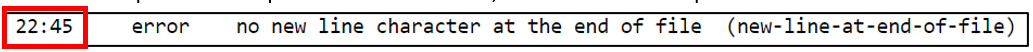
\includegraphics[width=16cm]{imagens/erroyaml.png}
	\caption{\label{fig:erroyaml} Exemplo de erro no yaml}
	\fonte{Os autores}
\end{figure}
\FloatBarrier

Elas representam, respectivamente, a linha e o caractere que apresentou o erro (ex: linha 22, caractere 45).


Esses foram os erros que conseguimos identificar conforme íamos tentando validar o nosso arquivo, então pode ser que há outros erros que não foram mapeados nessa postagem. 

Estamos abertos para a troca de experiências e esperamos ter ajudado :)

\section{Resumo de Atividades - Semana 11}
Na décima-primeira semana, entregamos e mostramos o documento final para o professor, que apontou alguns pontos de melhoria. Ele também alegou que o nosso arquivo equipe.yaml estava errado, pois não estava aparecendo no site da disciplina. Então fomos buscar mais a fundo sobre isso e conseguimos identificar os principais erros que podem aparecer na hora de validar um arquivo yaml. Assim, elaboramos um documento com esses principais erros, até mesmo para ajudar as próximas turmas da disciplina. 

No nosso checkpoint semanal, foi feito uma lista do que faltava para a aplicação ficar pronta e decidimos os próximos passos para cada integrante, que seria voltada para os ajustes no documento ou finalização da aplicação.

Além disso, ficamos sabendo que seríamos a primeira equipe a se apresentar (dia 26/07), então nos reunimos duas vezes para validar se estava tudo certo e também treinar para a apresentação final. 

Segue abaixo as atividades de cada integrante:

\begin{itemize}
\item André: fez a listagem de atividades e envio de anexos, a criação das conquistas, a entrega de atividades e de conquistas, o encerramento de turmas, correção na criação de atividades e o ranking
\item Bianca: ajustou o equipe.yaml, criou o documento dos erros do yaml, fez a apresentação do projeto e ajustou o documento final (segurança, escopo, manutenibilidade, métricas e apêndices)
\item Gustavo: fez a validação dos formulários de atividades e correções dos erros para a apresentação
\item Luiz: fez a geração do Latexdiff e os ajustes na documentação final (links de acesso, modelagem de dados, manutenibilidade, tecnologias e escopo)
\item Natan: gerou o vídeo do Gource, auxiliou na geração do Latexdiff e criou buscas dinâmicas dos registros da visão do administrador e do professor na tela do gestor
\item Patricia: fez os teste de alunos, de turmas, de conquistas e de atividades, o isolamento do firebase, a reorganização e a elaboração do roteiro de testes e montagem do backlog de correções
\end{itemize}

\section{Resumo de Atividades - Semana 12}
Na décima-segunda semana, apresentamos o nosso MVP para a banca. :)

Foi melhor que esperávamos, pois os pontos levantados pelos professores foram críticas construtivas que de fato estavam errados ou que irão agregar valor ao projeto. Desse modo, a semana foi destinada em discutir as melhorias para o documento final e para a aplicação.

Segue abaixo os pontos mais críticos citados:

\begin{itemize}
\item Aprofundamento da introdução e revisão de literatura;
\item Seguir a risca a metodologia ágil Scrum;
\item Ajustes no texto;
\item Boas práticas no código;
\item Melhor distribuição das tarefas.
\end{itemize}

No nosso checkpoint semanal, foi decidido os próximos passos para cada integrante, que seria:

\begin{itemize}
\item André: fazer um documento de boas práticas para o código
\item Bianca: cuidar da abordagem Scrum no projeto
\item Gustavo: ajustar as validações dos campos
\item Luiz: cuidar das alterações do documento para a entrega final
\item Natan: ajustar a internacionalização no código
\item Patricia: aumentar a cobertura de testes
\end{itemize}

Além disso, foi feito mais uma reunião, na qual o André passou as boas práticas mapeadas por ele para os demais integrantes, e também como ficaria o gerenciamento do projeto pelo GitHub.


\section{Resumo de Atividades - Semana 13}
Na décima-terceira semana, assistimos a apresentação da outra equipe e anotamos alguns pontos que também precisaríamos alterar no nosso projeto.

Como foi semana de provas das outras disciplinas, alteramos a data da nossa reunião semanal para domingo. Nessa reunião, abordamos os principais pontos de inconsistências para os ajustes finais do documento e da aplicação, e terminamos de ajustar o que faltava no nosso projeto.

Segue as atividades de cada integrante:

\begin{itemize}
\item André: implementou os tiers e fez os ajustes na aplicação
\item Bianca: fez os ajustes na documentação final
\item Gustavo: fez os ajustes na aplicação
\item Luiz: fez os ajustes na documentação final
\item Natan: fez os ajustes na aplicação
\item Patricia: aumentou a cobertura de teste
\end{itemize}
% ----------------------------------------------------------
\chapter{Protótipos das Telas}
\label{prototipos}
% ----------------------------------------------------------

\begin{figure}[htb]
    \centering
	
\includegraphics[width=16cm]{imagens/Geral-Login.png}
	\caption{\label{fig:login} Protótipo da Tela: Tela de Login}
	\fonte{Os autores}
\end{figure}
\FloatBarrier


\section{Visão do Administrador}

\begin{figure}[htb]
    \centering
	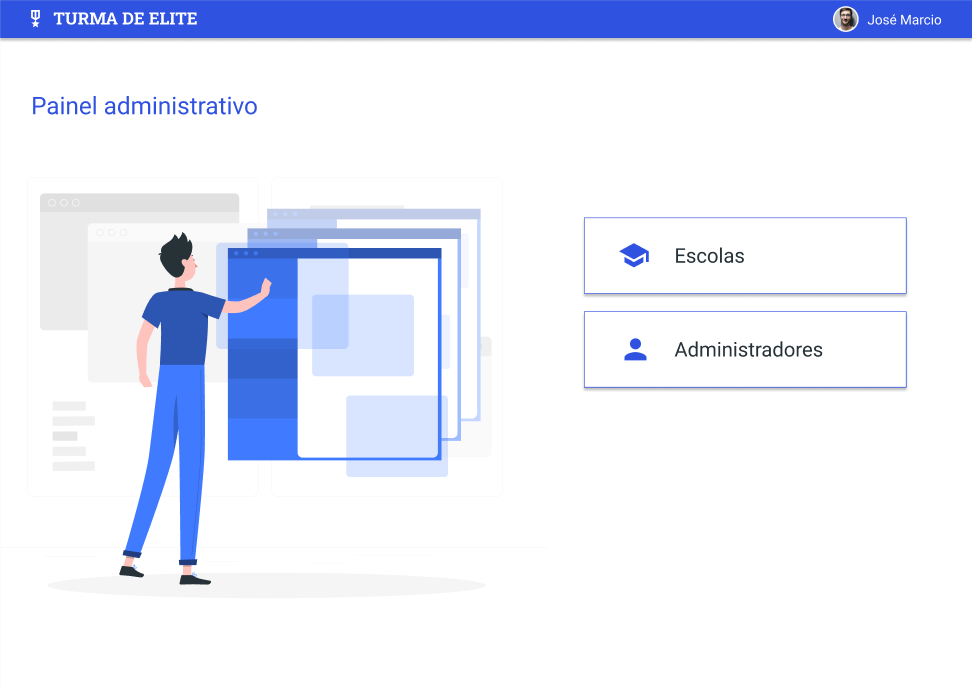
\includegraphics[width=16cm]{imagens/Administrador-PaginaInicial.png}
	\caption{\label{fig:administrador} Protótipo da Tela: Visão do Administrador - Página Inicial}
	\fonte{Os autores}
\end{figure}
\FloatBarrier

\begin{figure}[htb]
    \centering
	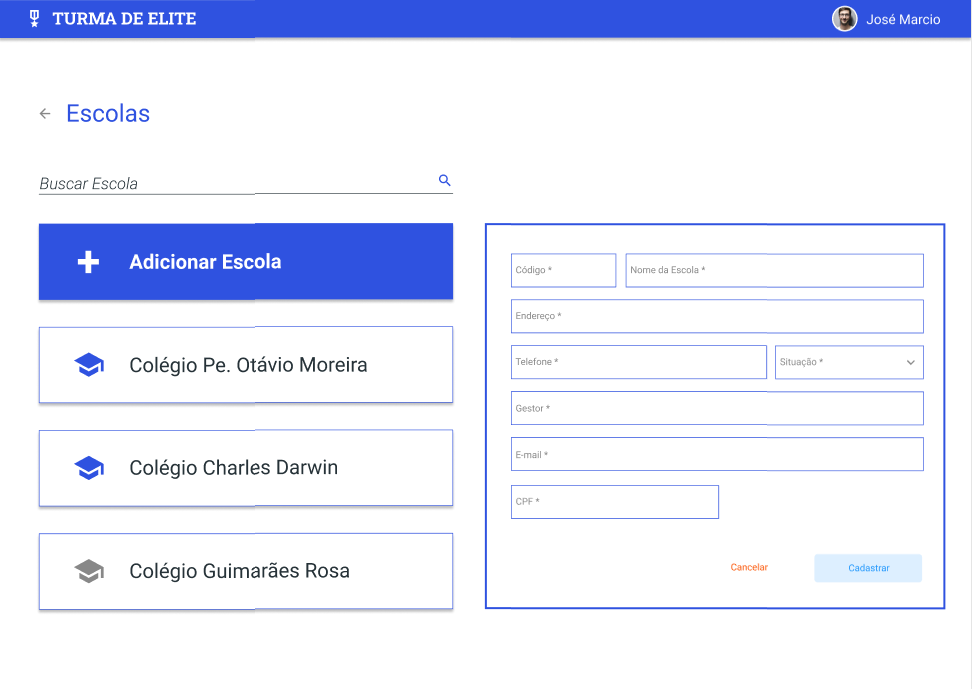
\includegraphics[width=16cm]{imagens/Administrador-CadastroEscola.png}
	\caption{\label{fig:cadastro-escola} Protótipo da Tela: Visão do Administrador - Cadastro de Escolas}
	\fonte{Os autores}
\end{figure}
\FloatBarrier

\begin{figure}[htb]
    \centering
	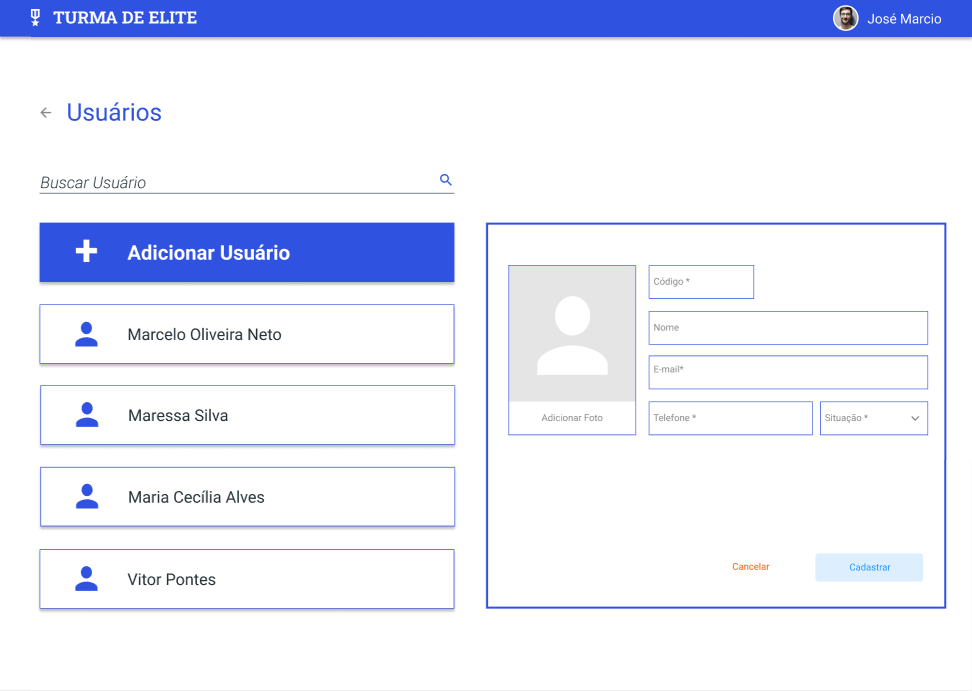
\includegraphics[width=16cm]{imagens/Administrador-CadastroUsuario.png}
	\caption{\label{fig:cadastro-usuário} Protótipo da Tela: Visão do Administrador - Cadastro de Usuários}
	\fonte{Os autores}
\end{figure}
\FloatBarrier


\section{Visão do Professor}

\begin{figure}[htb]
    \centering
	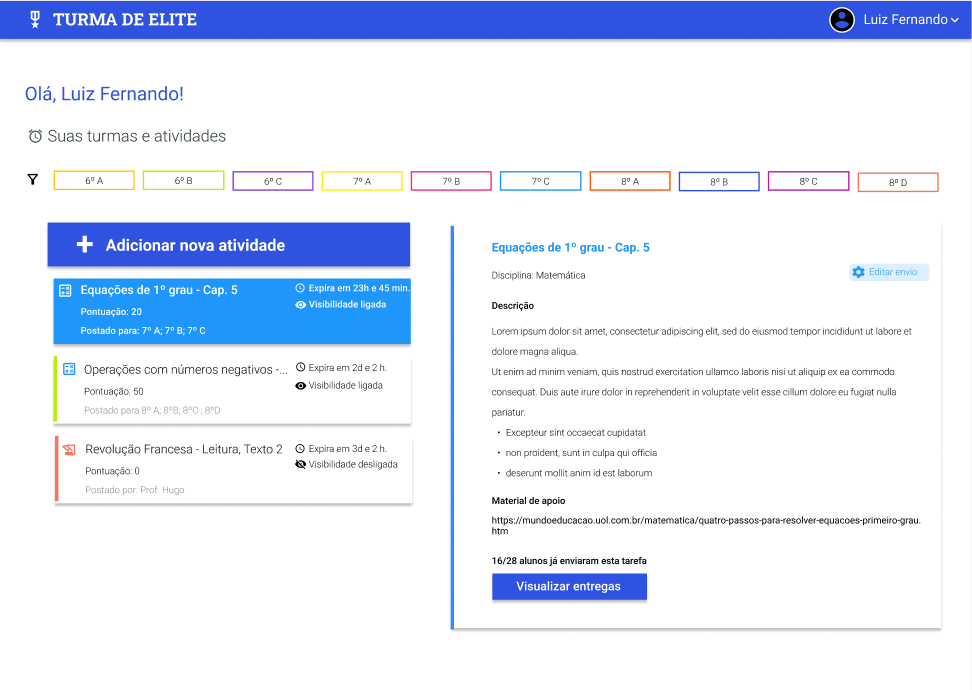
\includegraphics[width=16cm]{imagens/Professor-Atividades.png}
	\caption{\label{fig:atividades} Protótipo da Tela: Visão do Professor - Atividades}
	\fonte{Os autores}
\end{figure}
\FloatBarrier

\begin{figure}[htb]
    \centering
	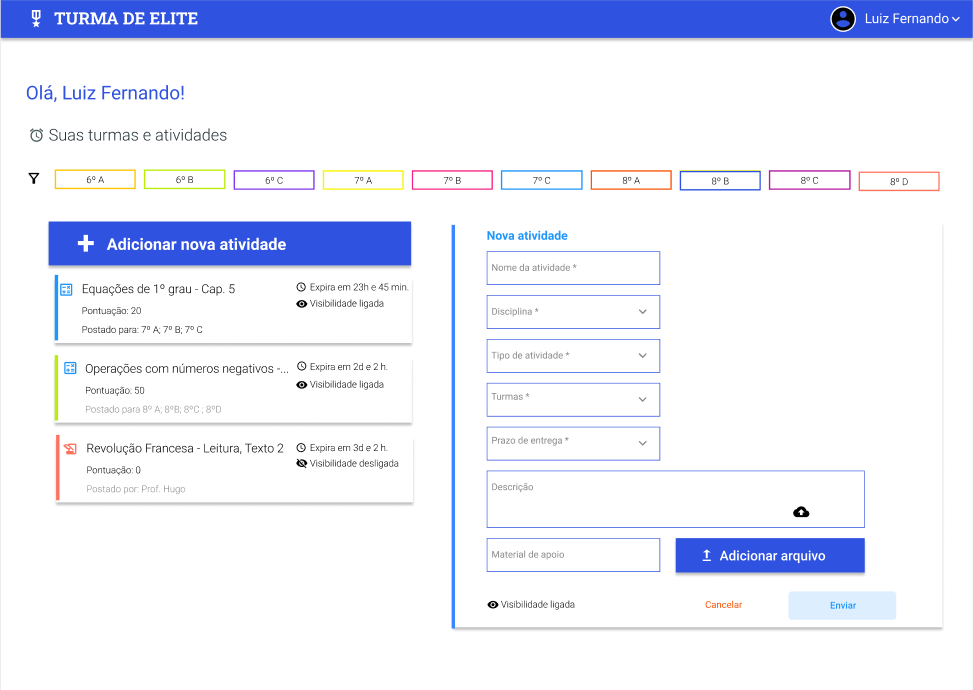
\includegraphics[width=16cm]{imagens/Professor-CadastroAtividades.png}
	\caption{\label{fig:professor} Protótipo da Tela: Visão do Professor - Cadastro de Atividades}
	\fonte{Os autores}
\end{figure}
\FloatBarrier


\section{Visão do Aluno}

\begin{figure}[htb]
    \centering
	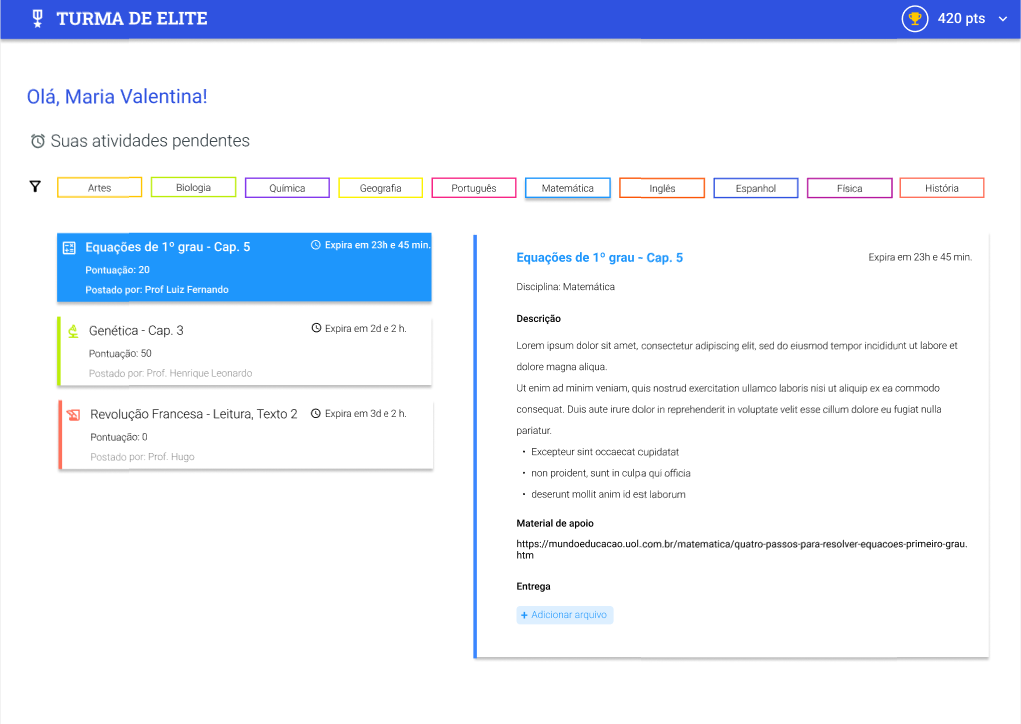
\includegraphics[width=16cm]{imagens/Aluno-Atividades.png}
	\caption{\label{fig:aluno} Protótipo da Tela: Visão do Aluno - Atividades}
	\fonte{Os autores}
\end{figure}
\FloatBarrier

\begin{figure}[htb]
    \centering
	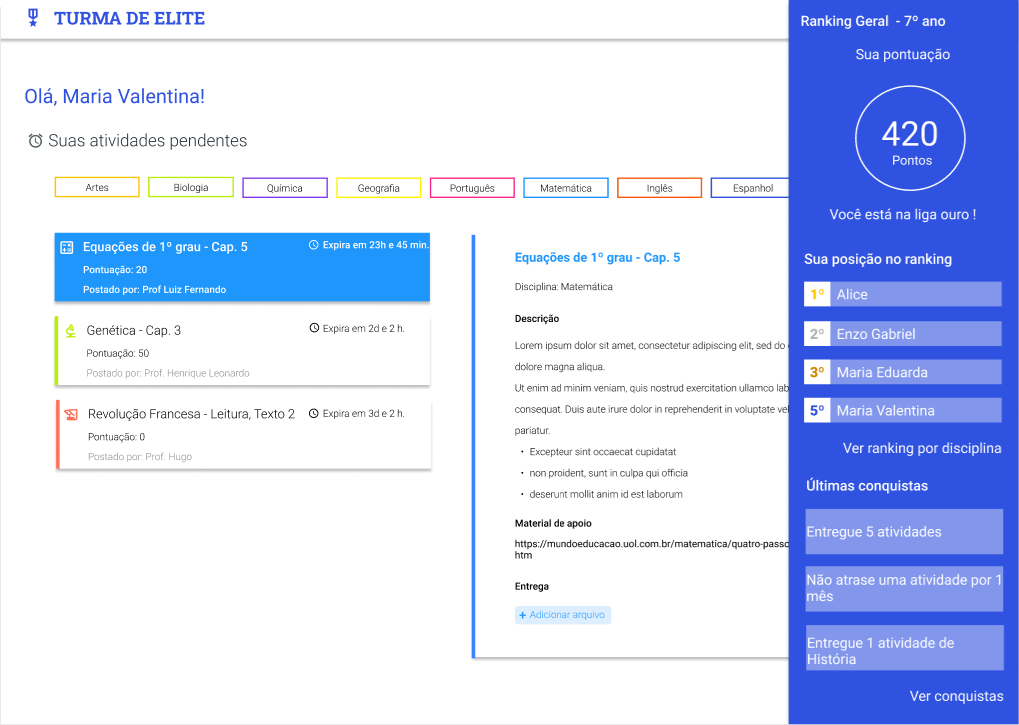
\includegraphics[width=16cm]{imagens/Aluno-MenuLateral.png}
	\caption{\label{fig:menu-lateral} Protótipo da Tela: Visão do Aluno - Menu Lateral}
	\fonte{Os autores}
\end{figure}
\FloatBarrier

\begin{figure}[htb]
    \centering
	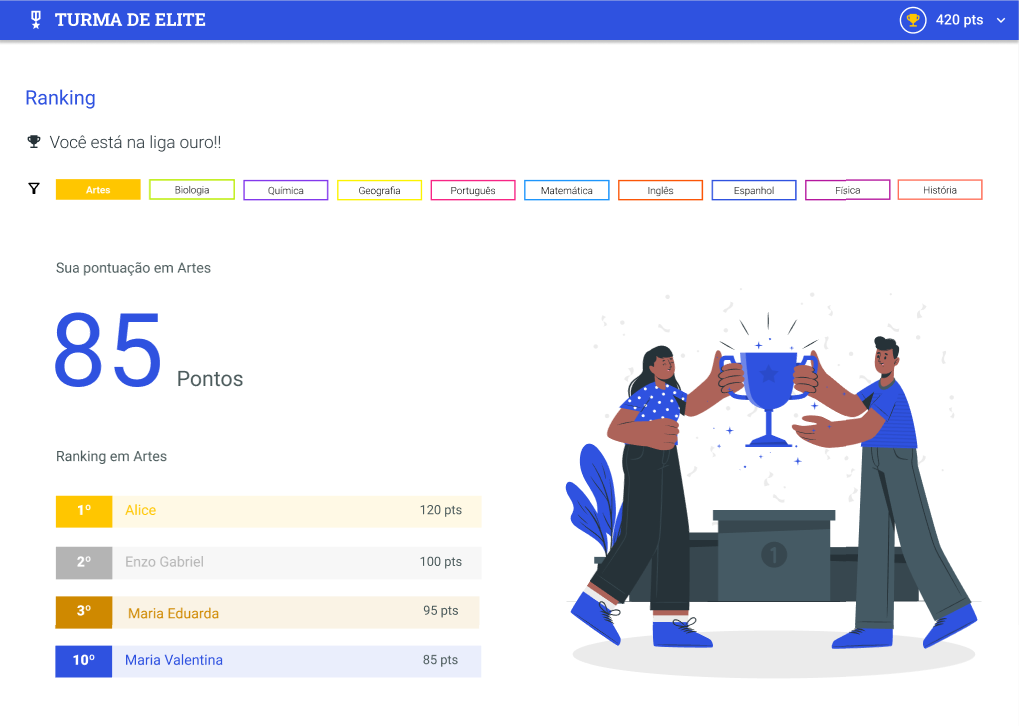
\includegraphics[width=16cm]{imagens/Aluno-Ranking.png}
	\caption{\label{fig:ranking} Protótipo da Tela: Visão do Aluno - Ranking}
	\fonte{Os autores}
\end{figure}
\FloatBarrier

\begin{figure}[htb]
    \centering
	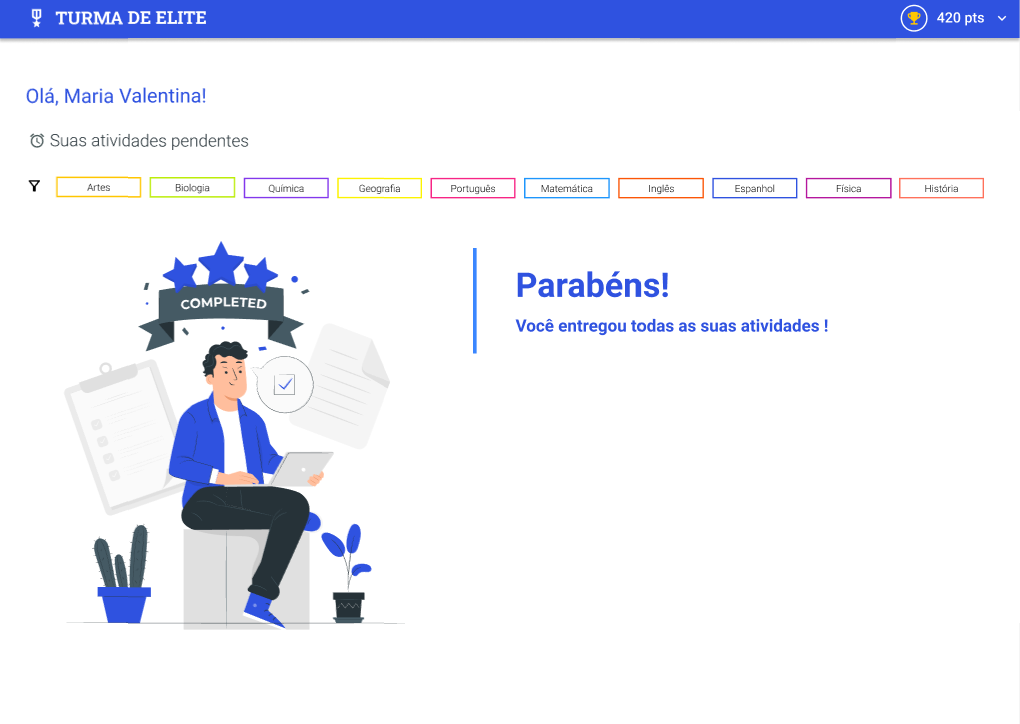
\includegraphics[width=16cm]{imagens/Aluno-Conquista.png}
	\caption{\label{fig:conquista} Protótipo da Tela: Visão do Aluno - Conquistas}
	\fonte{Os autores}
\end{figure}
\FloatBarrier


% ----------------------------------------------------------
\chapter{SSL Test - Back-end}
\label{ssltest-backend}
% ----------------------------------------------------------
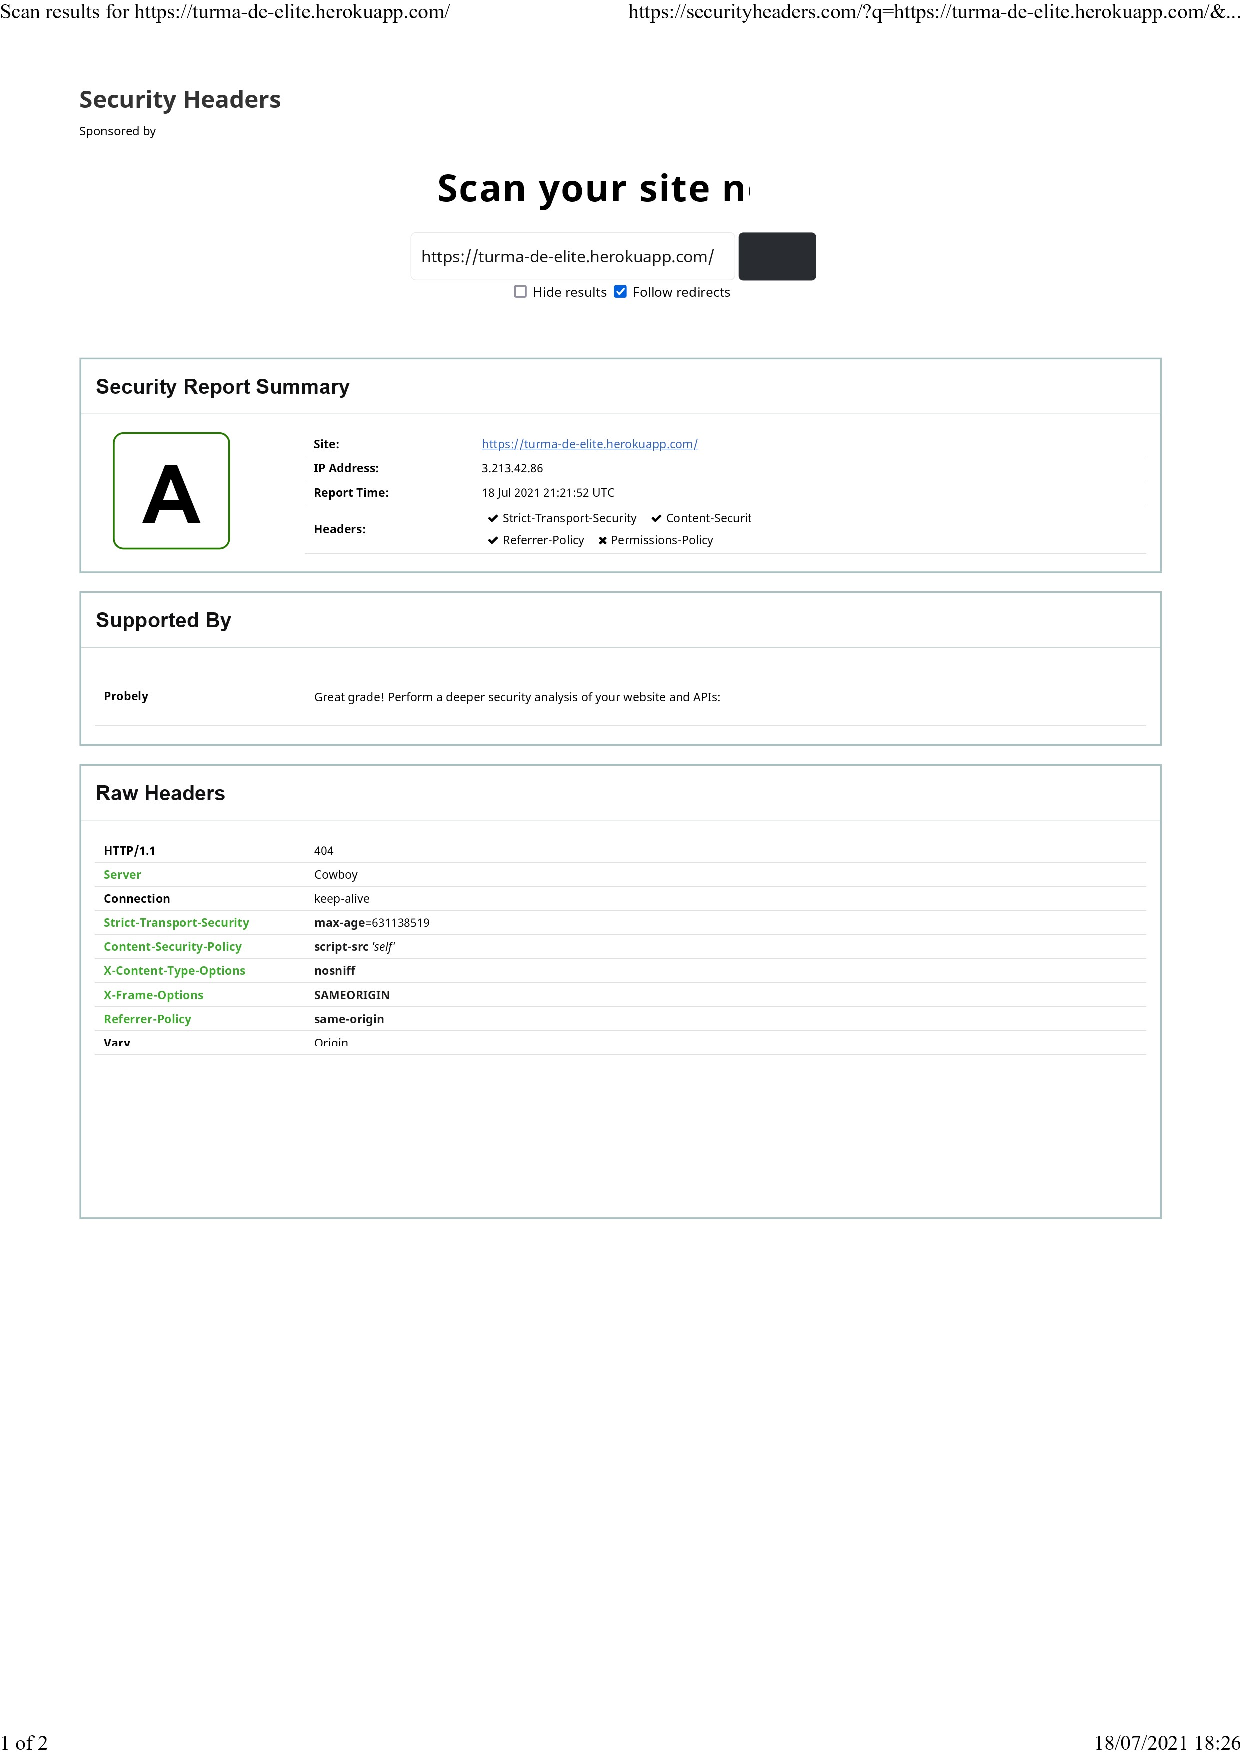
\includepdf[pages=-]{EntregaFinal/SECURITY_DOC.pdf}

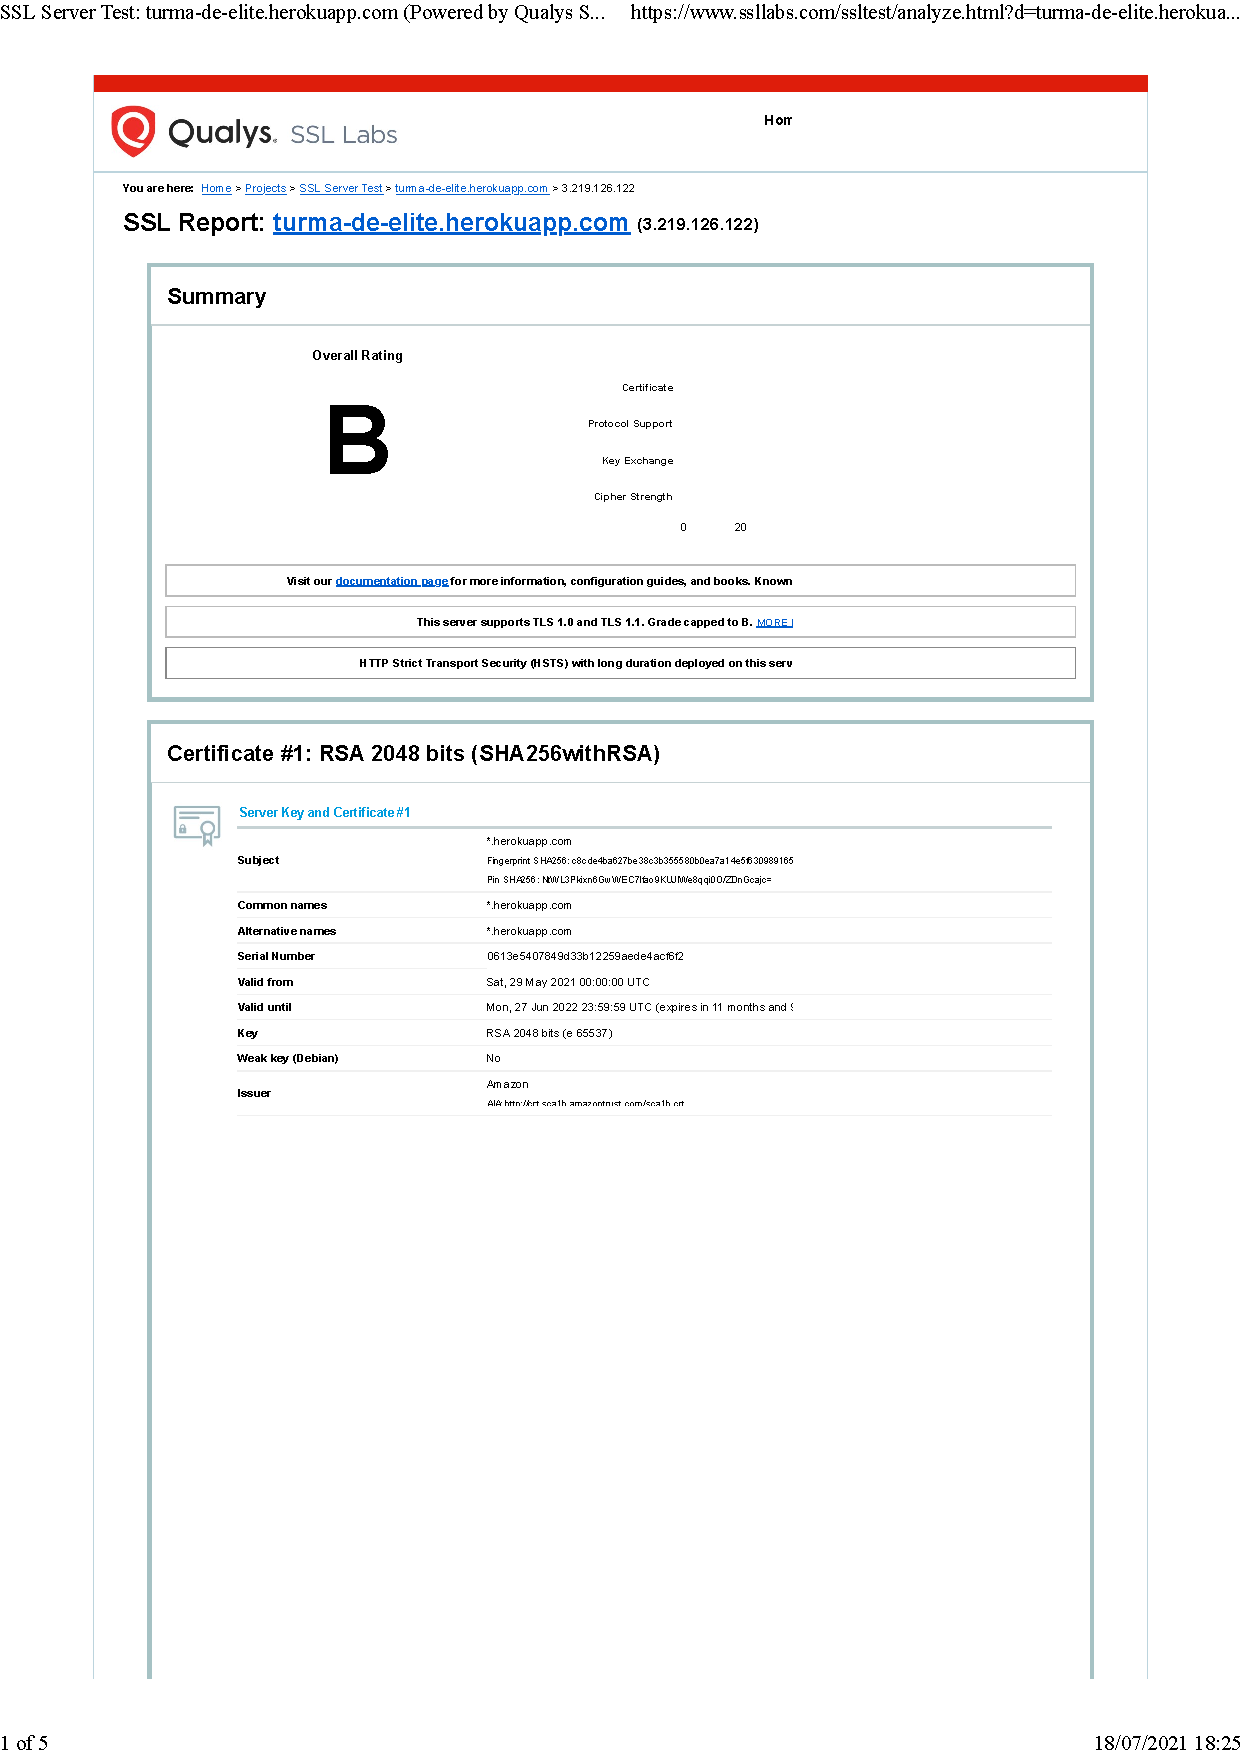
\includepdf[pages=-]{EntregaFinal/SSL_DOC.pdf}

% ----------------------------------------------------------
\chapter{SSL Test - Front-end}
\label{ssltest-frontend}
% ----------------------------------------------------------
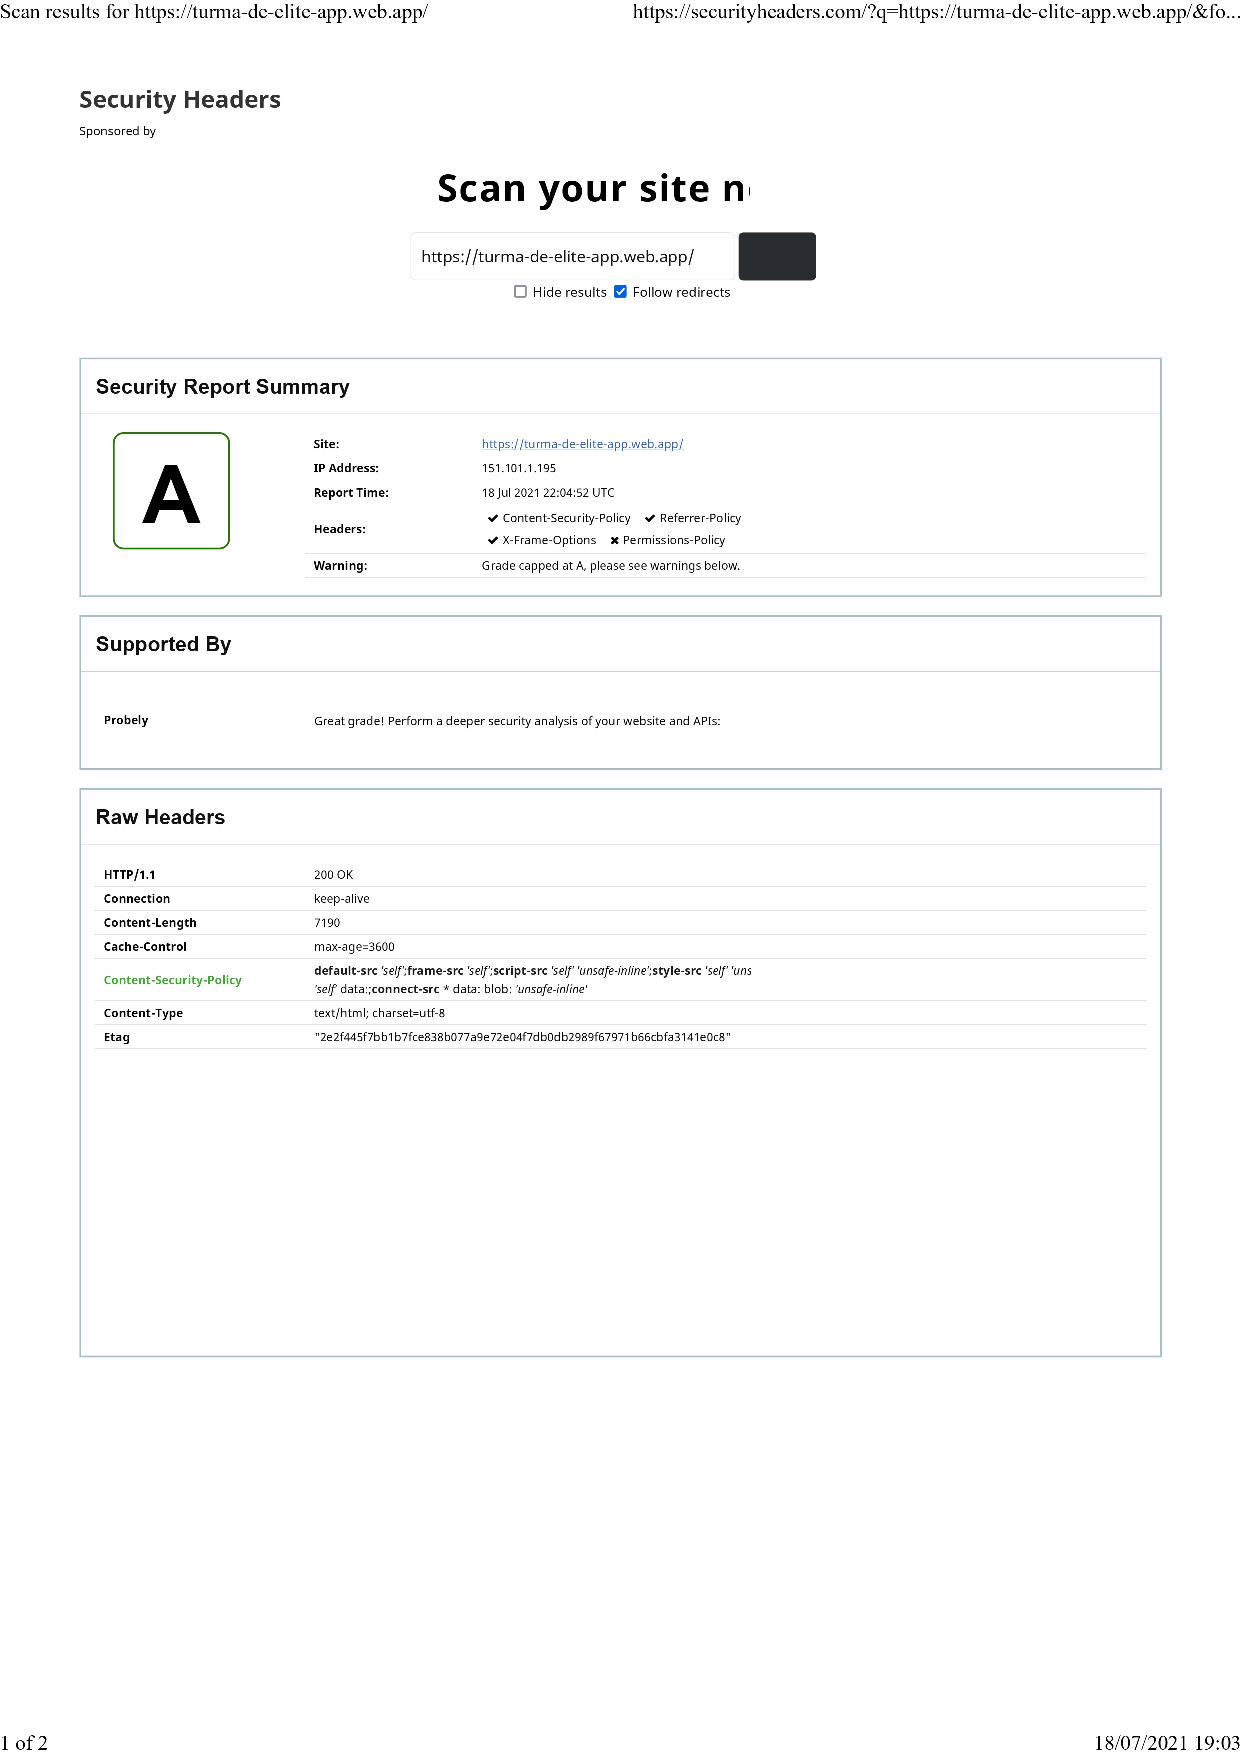
\includepdf[pages=-]{EntregaFinal/FRONT_END_SECURITY.pdf}

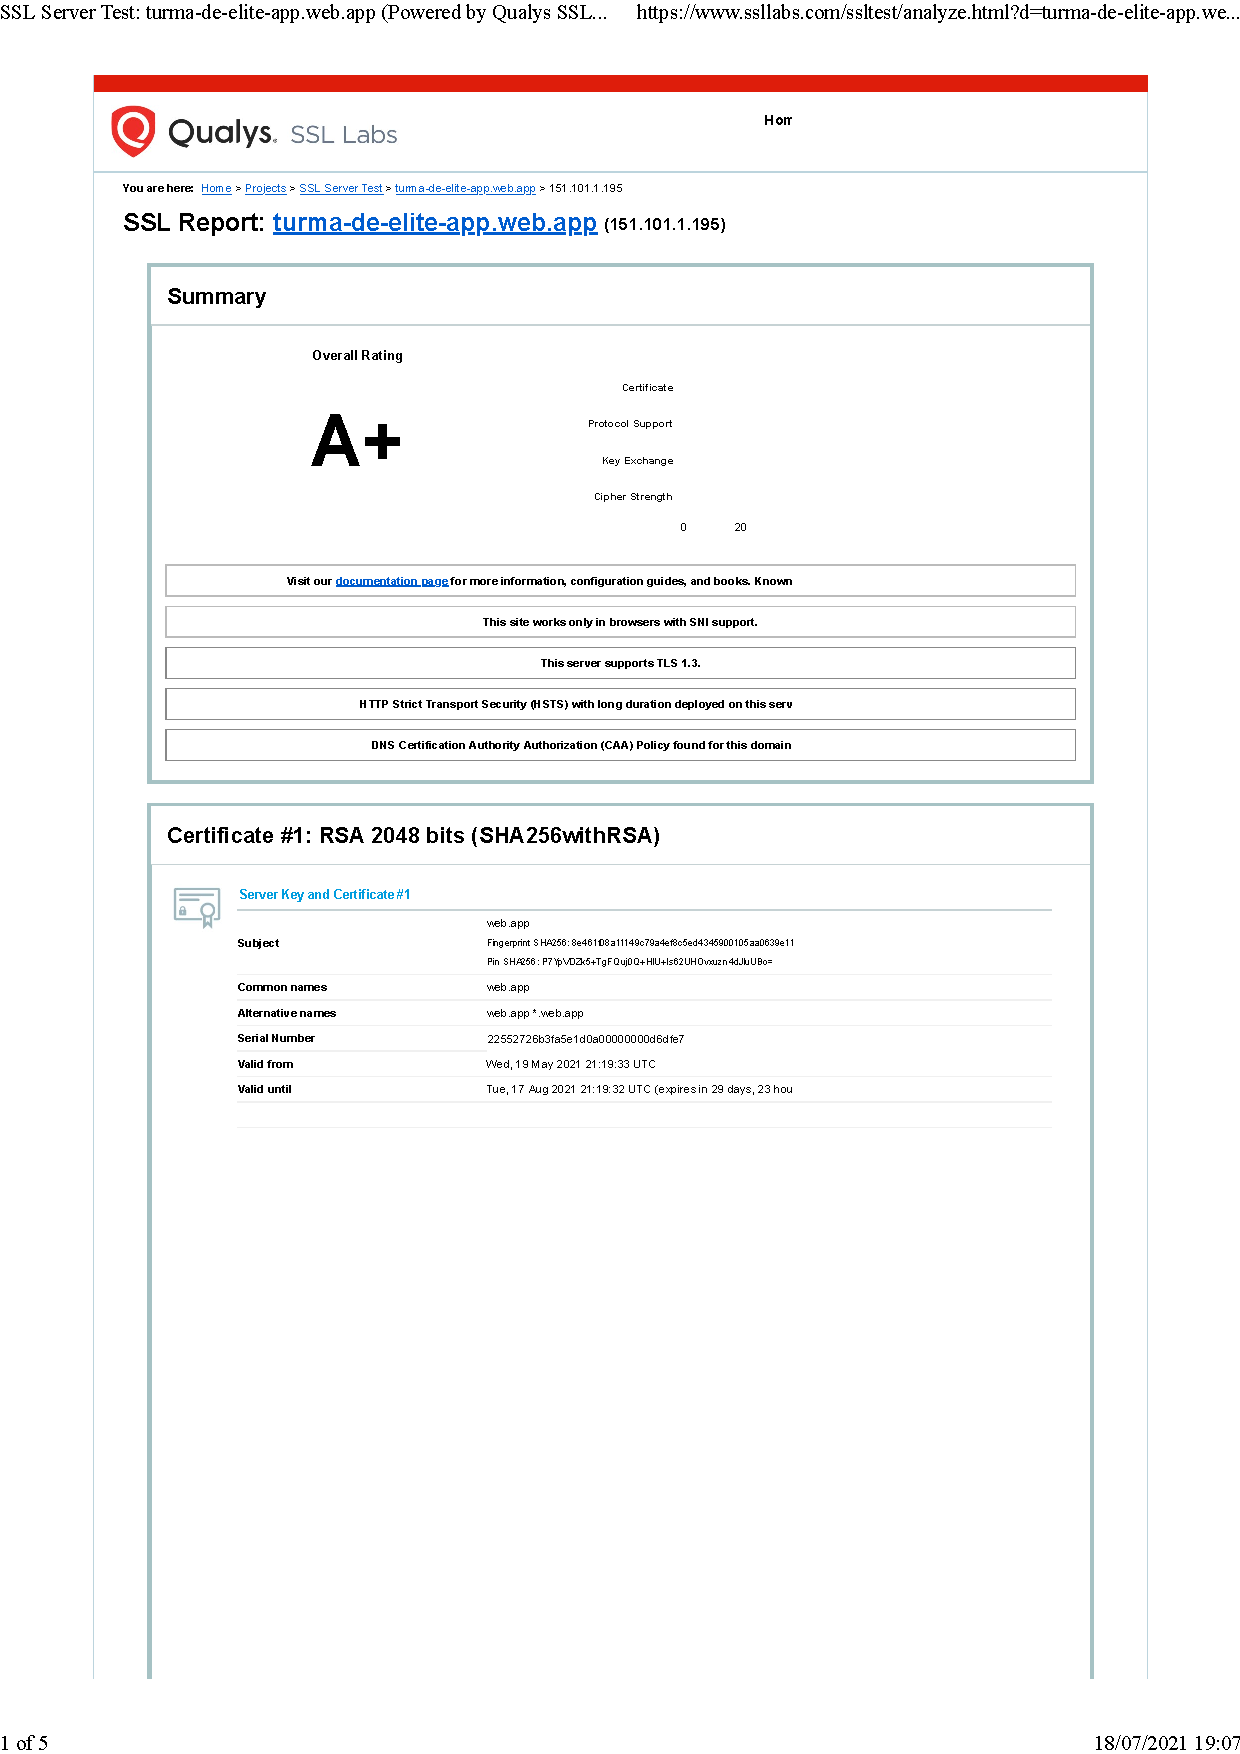
\includepdf[pages=-]{EntregaFinal/SSL_FRONT_DOC.pdf}
\end{apendicesenv}
% ---


%% ----------------------------------------------------------
% Anexos
% Documentos gerados por outros autores
% ----------------------------------------------------------

% ---
% Inicia os anexos
% ---
\begin{anexosenv}
\anexos
% Imprime uma página indicando o início dos anexos
\partanexos

% ---
\chapter{Manual todonotes(parcial)}
\label{manual-todonotes}
% ---
\index{pdf}
% se pages = "-"  fica com arquivo completo
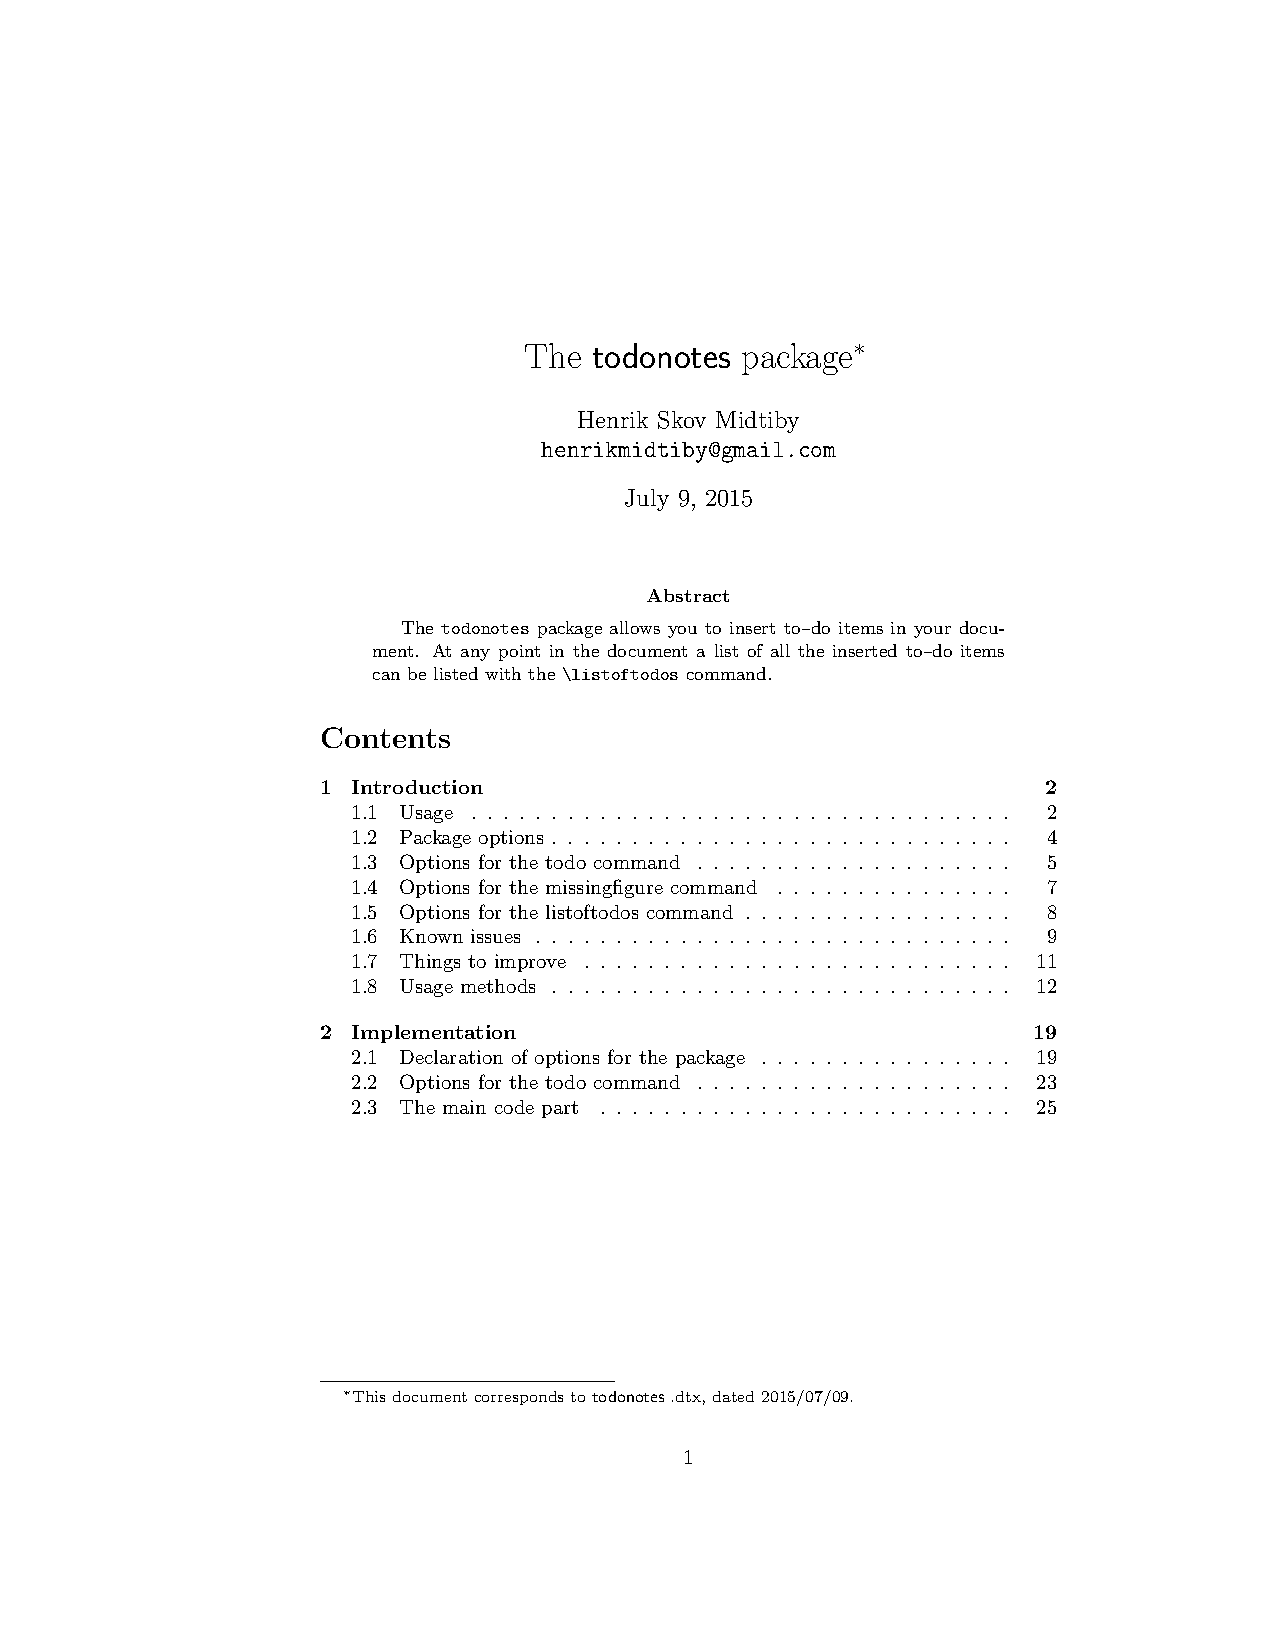
\includepdf[pages=1-3,scale=0.8,frame=true,pagecommand={}]{anexos/todonotes.pdf}

% ---
% Para incluir sem gerar a quebra de página inicial no anexo
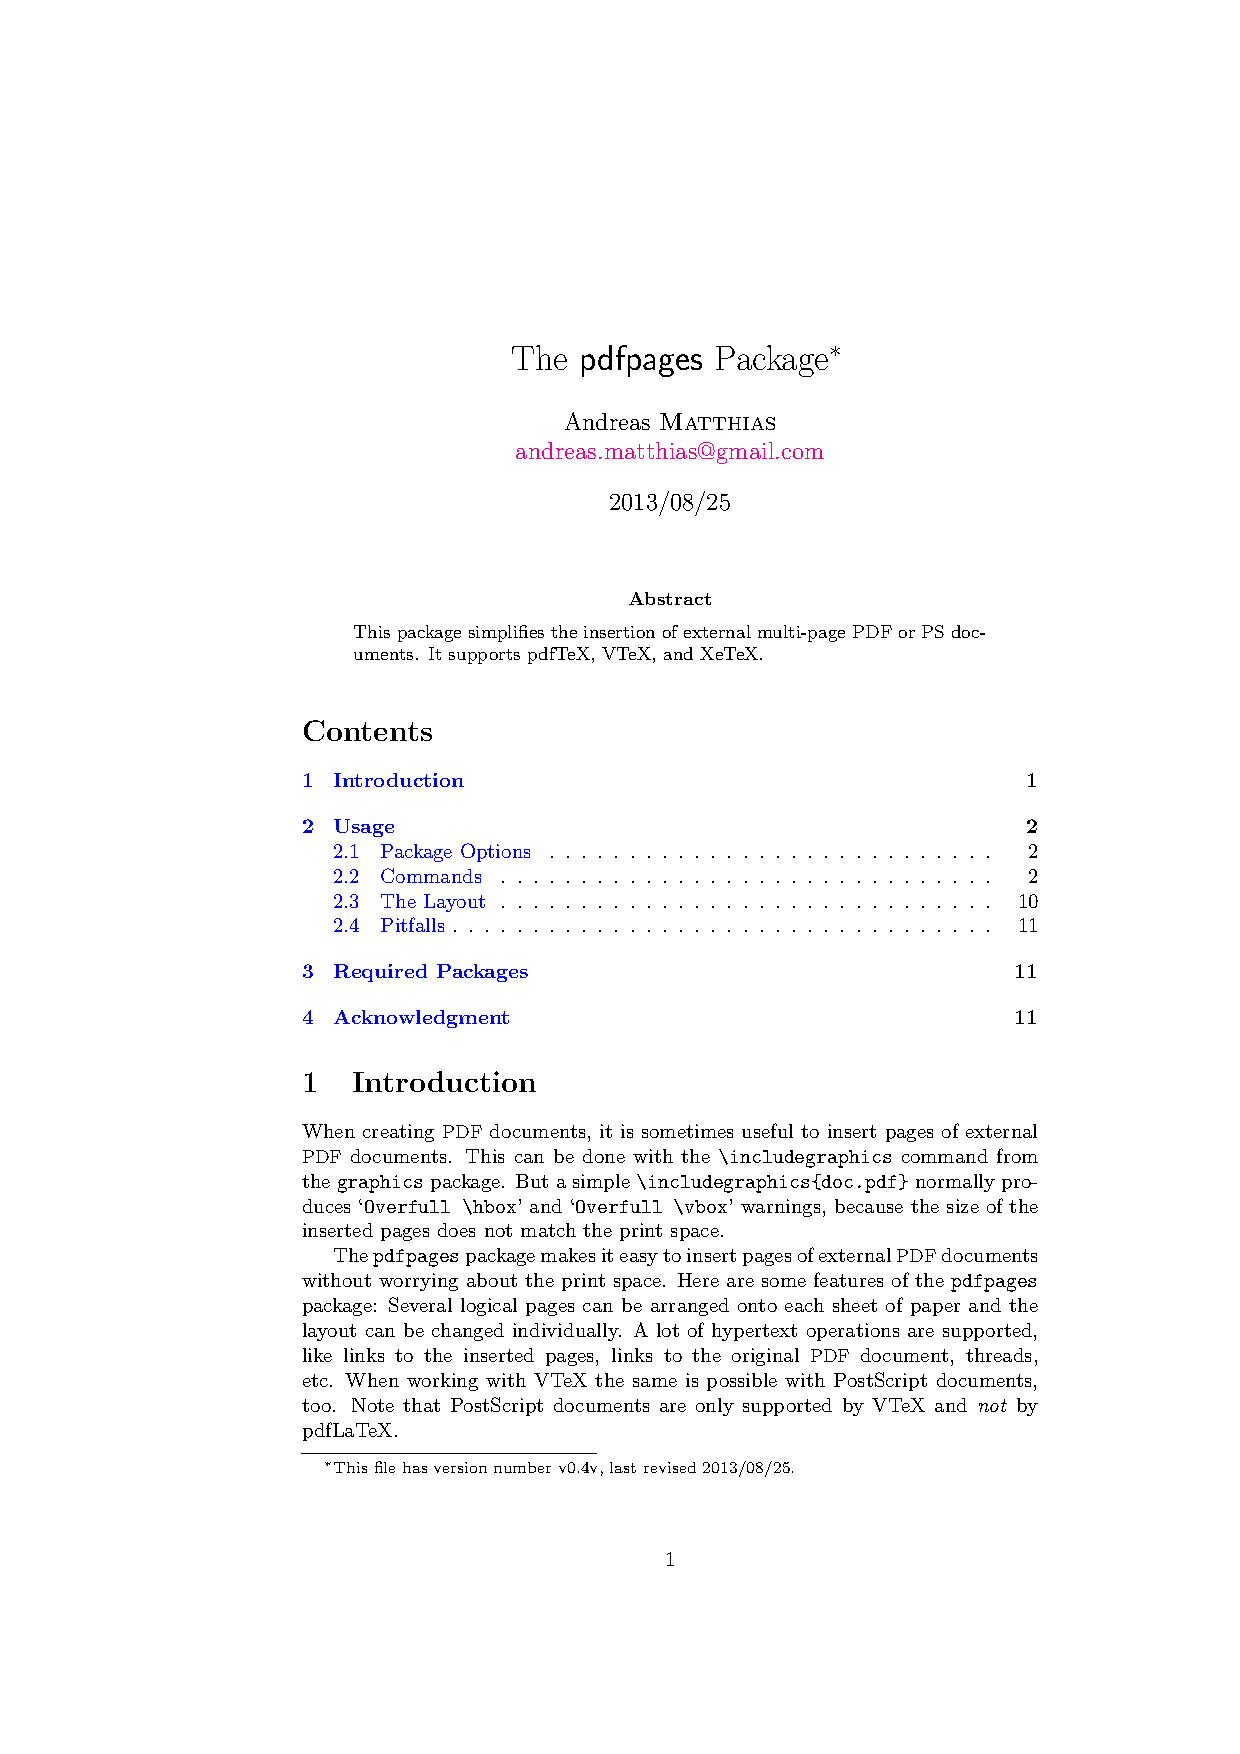
\includepdf[pages=1,scale=0.7,frame=true,pagecommand=\chapter{Manual pdfpages(parcial)}\label{manual-pdfpages}]{anexos/pdfpages.pdf}
\includepdf[pages=2-3,scale=0.8,frame=true,pagecommand={}]{anexos/pdfpages.pdf}

% ---
\chapter{Manual acronym(parcial)}
\index{pdf}
% somente algumas páginas para exemplo sem borda
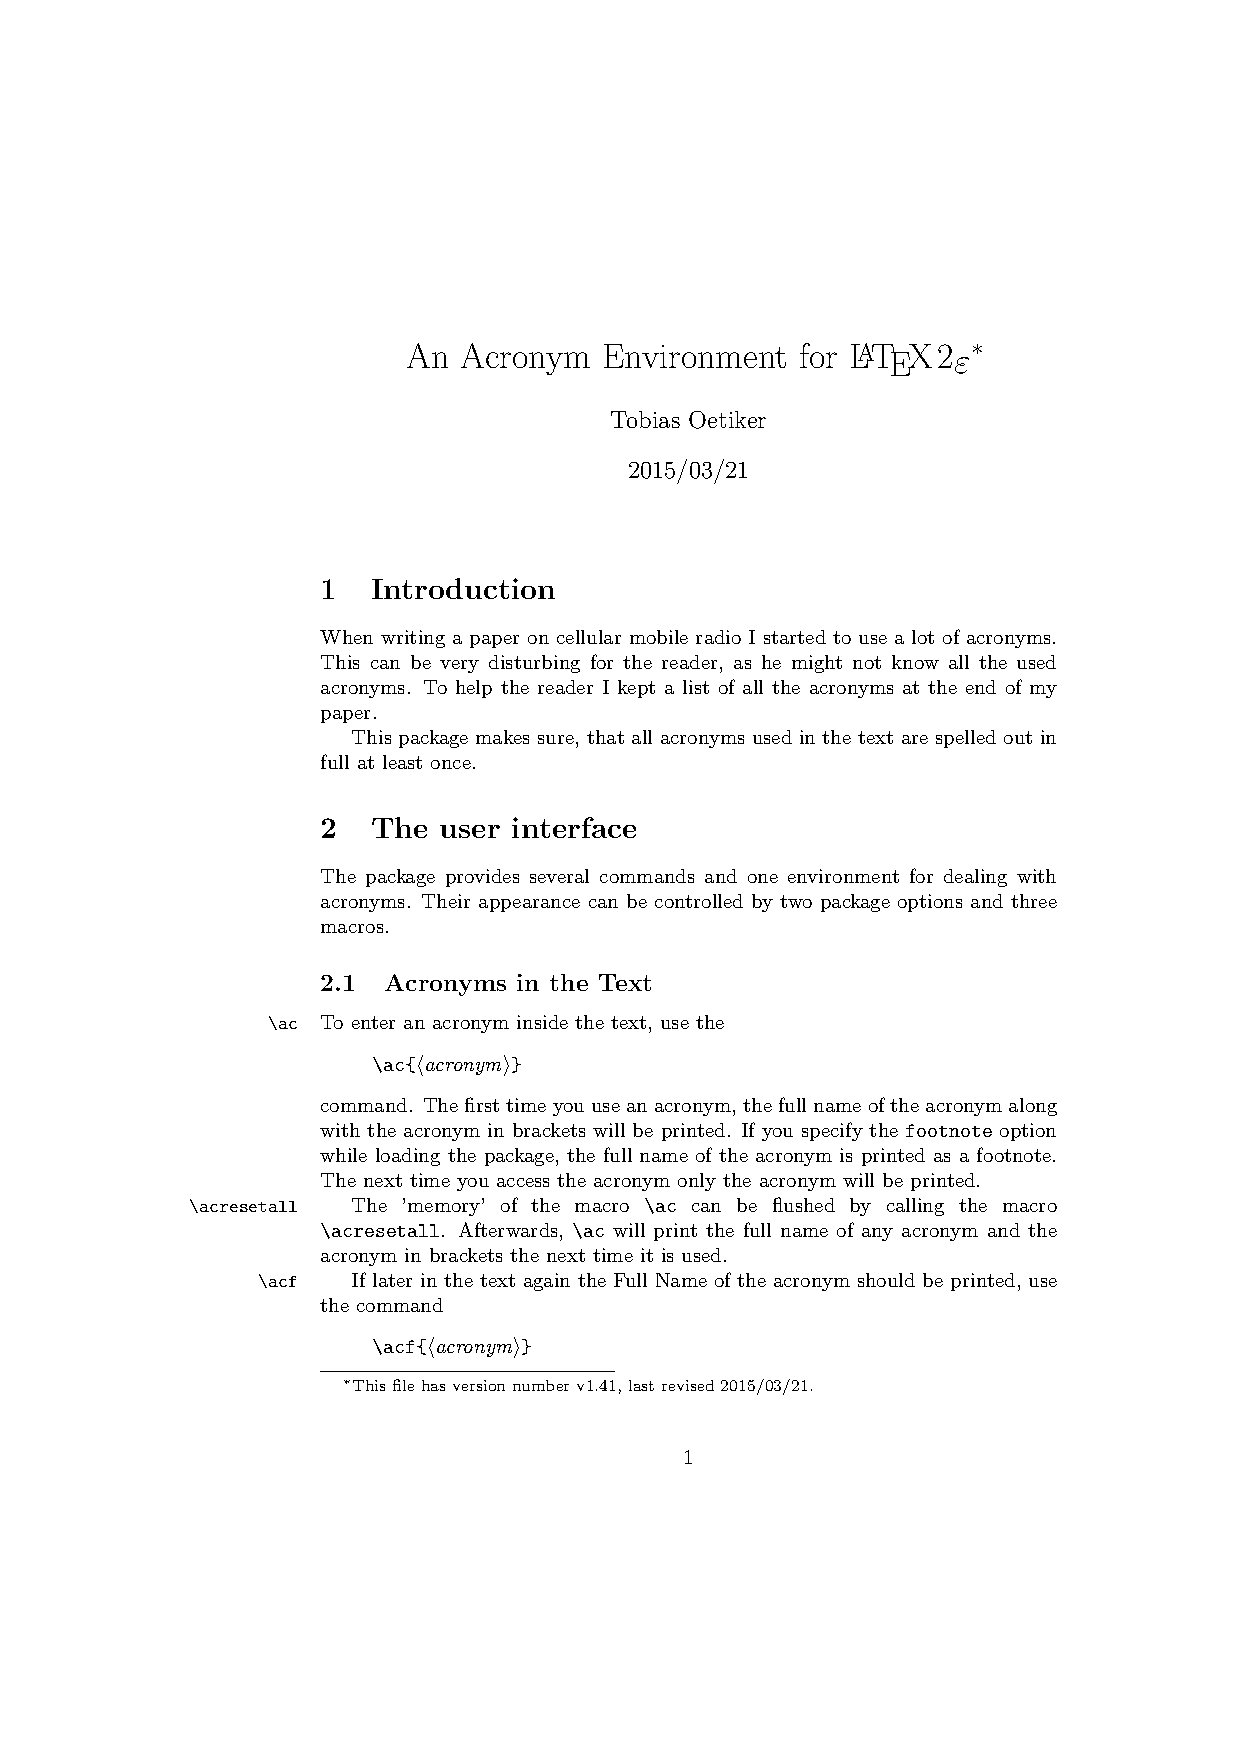
\includepdf[pages=1-3,frame=false,pagecommand={}]{anexos/acronym.pdf}



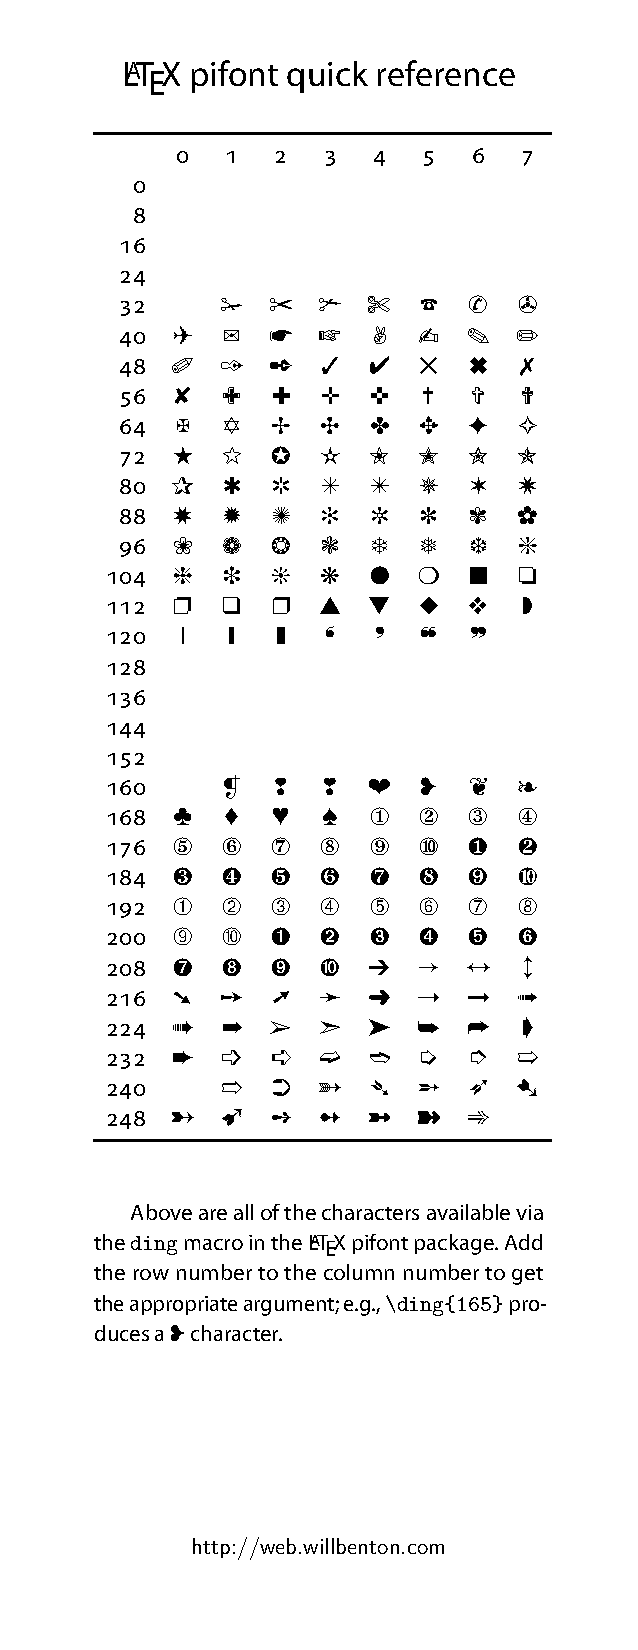
\includepdf[frame=true,scale=0.7,pagecommand=\chapter{Referência Rápida pifont}\label{pifont-quickref}]{anexos/pifont.pdf}


\end{anexosenv}



%---------------------------------------------------------------------
% INDICE REMISSIVO - Quando necessário 
% As palavras indexadas devem ser definidas com \index{} no texto
%---------------------------------------------------------------------
% \phantompart
% \printindex
% \todonum[inline]{remover indice remissivo se não for %necessário}

%---------------------------------------------------------------------

\end{document}